%%%%%%%%%%%%%%%%%%%%%%%%%%%%%%%%%%%%%%%%%%%%%%%%%%%%%%%%%%%%%%%%%%%%%%%%%%%%%%%%
% thesis.tex: Primary TeX control file for thesis.
%%%%%%%%%%%%%%%%%%%%%%%%%%%%%%%%%%%%%%%%%%%%%%%%%%%%%%%%%%%%%%%%%%%%%%%%%%%%%%%%
\documentclass[11pt, oneside]{mnthesis}
\usepackage{epsfig,epic,eepic,units}
\usepackage{hyperref}
\usepackage{url}
\usepackage{longtable}
\usepackage{tabularx} % better space usage with Tables
\usepackage{mathrsfs}
\usepackage{multirow}
\usepackage{bigstrut}
\usepackage{amssymb}
\usepackage{amsmath}
\usepackage{hyperref}
\usepackage{bookmark}
\usepackage{xspace}   % for forcing space after the command
%\usepackage{siunitx}  % for decimal alignment in the table
\usepackage[colorinlistoftodos, textwidth=3cm, textsize=tiny]{todonotes} % for notes
\usepackage{caption}
\DeclareCaptionFormat{myformat}{#1#2#3\hrulefill}

%manage algorithms
\usepackage[ruled,vlined]{algorithm2e} 

\usepackage{graphicx}
\usepackage[caption=false]{subfig}
\usepackage{tikz}
\usetikzlibrary{shapes.geometric, shapes.symbols,patterns, arrows, backgrounds, calc, fit, shapes.multipart, chains}
\tikzstyle{block} = [rectangle, draw, fill=blue!20, text width=10em, text centered, rounded corners, minimum height=4em]
\tikzstyle{line} = [draw, very thick, -latex']
\tikzstyle{cloud} = [draw, ellipse,fill=red!20, text width=8em, text centered,  minimum height=3em]


\newtheorem{definition}{Definition}
\newtheorem{assumption}{Assumption}
\newtheorem{observation}{Observation}

\providecommand{\abs}[1]{\lvert#1\rvert}

%%%%%%%%%%%%%%%%%%%%%%%%%%%%%%%%%%%%%%%%%%%%%%%%%%%%%%%%%%%%%%%%%%%%%%%%%%%%%%%%
% Custom definitions
%%%%%%%%%%%%%%%%%%%%%%%%%%%%%%%%%%%%%%%%%%%%%%%%%%%%%%%%%%%%%%%%%%%%%%%%%%%%%%%%
\newcommand{\C}{{\mathrm{c}}}

\newcommand{\COS}{{\mathrm{cos}}}
\newcommand{\SIN}{{\mathrm{sin}}}
\newcommand{\DOF}{{\mathrm{dof}}}
\newcommand{\MSEC}{\mu{\mathrm{s}}}
\newcommand{\NS}{\mathrm{ns}}
\newcommand{\PPM}{{\mathrm{ppm}}}
\newcommand{\ENR}{{\mathrm{GeV}}}
\newcommand{\MOM}{{\mathrm{GeV/c}}}

\newcommand{\CONT}{\noindent}
\newcommand{\SEC}{Sec.\ }
\newcommand{\SECS}{Secs.\ }
\newcommand{\EQ}{Eq.\ }
\newcommand{\EQS}{Eqs.\ }
\newcommand{\APP}{Appendix }
\newcommand{\APPS}{Appendices }
\newcommand{\CHP}{Chapter}
\newcommand{\CHPS}{Chapters }

\newcommand{\pesto}{Pesto\xspace}
\newcommand{\basil}{Basil\xspace}
\newcommand{\romano}{Romano\xspace}
\newcommand{\RAND}{X}
\newcommand{\READ}{R}
\newcommand{\OIO}{O}
\newcommand{\SIZE}{Z}

\newcounter{todocounter}
\newcommand{\nohhyun}[2][]{
  \stepcounter{todocounter}
  \todo[#1, color=blue!20]{\textbf{\thetodocounter:} #2}
}
%%%%%%%%%%%%%%%%%%%%%%%%%%%%%%%%%%%%%%%%%%%%%%%%%%%%%%%%%%%%%%%%%%%%%%%%%%%%%%%%


\linespread{1.3}
\begin{document}
\bibliographystyle{hunsrt} % style of bibliography
%%%%%%%%%%%%%%%%%%%%%%%%%%%%%%%%%%%%%%%%%%%%%%%%%%%%%%%%%%%%%%%%%%%%%%%%%%%%%%%%

%%%%%%%%%%%%%%%%%%%%%%%%%%%%%%%%%%%%%%%%%%%%%%%%%%%%%%%%%%%%%%%%%%%%%%%%%%%%%%%%
% Title and other sections that come before the body of the document
%%%%%%%%%%%%%%%%%%%%%%%%%%%%%%%%%%%%%%%%%%%%%%%%%%%%%%%%%%%%%%%%%%%%%%%%%%%%%%%%
%%%%%%%%%%%%%%%%%%%%%%%%%%%%%%%%%%%%%%%%%%%%%%%%%%%%%%%%%%%%%%%%%%%%%%%%%%%%%%%%
% title.tex - Set up the beginning of thesis.
%%%%%%%%%%%%%%%%%%%%%%%%%%%%%%%%%%%%%%%%%%%%%%%%%%%%%%%%%%%%%%%%%%%%%%%%%%%%%%%%
% For a  PhD give the command \phd. Default is masters
%\degree (normally Doctor of Philosophy or Master of Science)
%\initials (normally Ph.D. or M.S.)
%\ms % use if for a Master of Science thesis
\phd % use if for a Ph.D. dissertation
%\draft

\title{\bf Statistical Characterization of Storage System Workloads
\\
for Data Deduplication and Load Placement 
\\
in Heterogeneous Storage Environments}
\author{Nohhyun Park}
\campus{University of Minnesota} 
\program{Electrical and Computer Engineering} 
\director{David J. Lilja} 

% Optionally specify the month and year.
%\submissionmonth{August} % defaults to current month.
%\submissionyear{2012} % defaults to current year.

%Comment out below on final copy
\abstract{%%%%%%%%%%%%%%%%%%%%%%%%%%%%%%%%%%%%%%%%%%%%%%%%%%%%%%%%%%%%%%%%%%%%%%%%%%%%%%%%
% abstract.tex: Abstract
%%%%%%%%%%%%%%%%%%%%%%%%%%%%%%%%%%%%%%%%%%%%%%%%%%%%%%%%%%%%%%%%%%%%%%%%%%%%%%%%

The underlying technologies for storing digital bits have become more diverse in last decade. 
There is no fundamental differences in their functionality yet their behaviors can be quite different and no single management technique seems to fit them all. 
The differences can be categorized based on the metric of interest such as the performance profile, the reliability profile and the power profile.
 
These profiles are a function of the system and the workload assuming that the systems are exposed only to a pre-specified environment. 
Near infinite workload space makes it infeasible to obtain the complete profiles for any storage systems unless the system enforces a discrete and finite profile internally.
The thesis of this work is that an acceptable approximation of the profiles may be achieved by proper characterization of the workloads. 
A set of statistical tools as well as understanding of system behavior were used to evaluate and design such characterizations. 
The correctness of the characterization cannot be fully proved except by showing that the resulting profile can correctly predict any workload and storage system interactions. 
While this is not possible, we show that we can provide a reasonable confidence in our characterization by statistical evaluation of results. 

The characterizations of this work were applied to compression ratio for backup data deduplication and load balancing of heterogeneous storage systems in a virtualized environments. 
The validation of our characterization is validated through hundreds of real world test cases as well as reasonable deductions based on our understanding of the storage systems. 
In both cases, the \emph{goodness} of characterizations were rigorously evaluated using statistical techniques.
The findings along the validations were both confirming and contradicting of many previous beliefs. 

%%%%%%%%%%%%%%%%%%%%%%%%%%%%%%%%%%%%%%%%%%%%%%%%%%%%%%%%%%%%%%%%%%%%%%%%%%%%%%%%
}
\words{331}    % number of words in the abstract
\acknowledgements{%%%%%%%%%%%%%%%%%%%%%%%%%%%%%%%%%%%%%%%%%%%%%%%%%%%%%%%%%%%%%%%%%%%%%%%%%%%%%%%%
% acknowledge.tex: Acknowledgements
%%%%%%%%%%%%%%%%%%%%%%%%%%%%%%%%%%%%%%%%%%%%%%%%%%%%%%%%%%%%%%%%%%%%%%%%%%%%%%%%

I like to thank my advisor, David J. Lilja, who has suffered through more than a handful insensible ideas and lack of experience. Also members of ARCTiC lab, Biplob Debnath, Shruti Patil, Eric Seppanen, Weijun Xiao, Peng Li and William Tuohy for their friendship and insights. 

My thanks also goes to student members of CRIS, Weiping He, Anna Kryzhnyaya, Muthukumar Murugan, Joe Naps, Dongchul Park and Guanlin Lu for interesting projects and fun trips. 

I would also like to thank my committee members, David Du, Ulya Karpuzcu and John Sartori for their valuable comments and guidance. 
 
I would like to thank Jerry Fredin of NetApp for his support during the data deduplication project. 
I also like to thank Philip Shilain and Fred Douglis of EMC for their feedbacks on numerous projects. 
I would like to thank Dave B. Anderson and Luke W. Friendshuh for their support during the IO workload characterization project.
I would also like to thank Irfan Ahmed and DRS team at VMware for their support during the Romano project. 

I would like to thank DARPA, NSF and CRIS member companies for funding my projects as well as Minnesota Supercomputing Institute for providing the valuable compute cycles. 

I would also like to mention Sungwook and Sangyeon Jeong whom I promised to include in my acknowledgement in exchange for occasional free lunch at their place. 

I could not have survived long years of graduate school without the support of my parents whose interest in technology and willingness to invest in my education allowed me to find and pursue my passion. 

Although mostly distraction then help, I would also like to thank my brother, Nohguen, for the occasional fun times we were able to have in last 6 years. 

My special thanks goes to Hyewon and Ciana. 

%%%%%%%%%%%%%%%%%%%%%%%%%%%%%%%%%%%%%%%%%%%%%%%%%%%%%%%%%%%%%%%%%%%%%%%%%%%%%%%%
}
\dedication{To my parents.
}
%
% Use a special preface
%\extra{\input{preface}}

% The \beforepreface command actually causes insertion of the title, 
% abstract, signature, and copyright pages into the new document.
\beforepreface 

% Define the text to go before the table of contents
\figurespage
\tablespage

% The \afterpreface command actually causes insertion of the
% contents, list of figures, etc. into the new document.
\afterpreface            
%%%%%%%%%%%%%%%%%%%%%%%%%%%%%%%%%%%%%%%%%%%%%%%%%%%%%%%%%%%%%%%%%%%%%%%%%%%%%%%%

%%%%%%%%%%%%%%%%%%%%%%%%%%%%%%%%%%%%%%%%%%%%%%%%%%%%%%%%%%%%%%%%%%%%%%%%%%%%%%%%

%%%%%%%%%%%%%%%%%%%%%%%%%%%%%%%%%%%%%%%%%%%%%%%%%%%%%%%%%%%%%%%%%%%%%%%%%%%%%%%%
% Now lets include the body of the document...
%%%%%%%%%%%%%%%%%%%%%%%%%%%%%%%%%%%%%%%%%%%%%%%%%%%%%%%%%%%%%%%%%%%%%%%%%%%%%%%%
%%%%%%%%%%%%%%%%%%%%%%%%%%%%%%%%%%%%%%%%%%%%%%%%%%%%%%%%%%%%%%%%%%%%%%%%%%%%%%%
% intro.tex: Introduction to the thesis
%%%%%%%%%%%%%%%%%%%%%%%%%%%%%%%%%%%%%%%%%%%%%%%%%%%%%%%%%%%%%%%%%%%%%%%%%%%%%%%%
\chapter{Introduction}
\label{intro_chapter}
%%%%%%%%%%%%%%%%%%%%%%%%%%%%%%%%%%%%%%%%%%%%%%%%%%%%%%%%%%%%%%%%%%%%%%%%%%%%%%%%
\section{Motivation}
\label{motivation}


\section{Problem Statement}
\label{problem}

\cite{wood2007black}

\section{Outline}
\label{outline}
\begin{itemize}

%\item Chapter 1 introduces the analytic goals pursued in this thesis.

\item Chapter 2 briefly presents the history of, and science behind, the
subjects presented in this thesis.

\item In Chapter 3 the experiment is outlined.

\item Chapter 4 describes the simulation process used in the analysis.

\item Chapter 5 follows the chain of reconstruction software used to obtain
meaningful results from data.

\item Chapter 6 hashes out the strategy for analysis and presents the data and
simulated sets that will be used in the analysis.

\item Chapter 7 demonstrates the implementation of the event selection
processes.

\item In Chapter 8 those events selected in Chapter 7 are analyzed.

\item Chapter 9 presents a final discussion of the analyses presented in the
thesis.

\end{itemize}
%%%%%%%%%%%%%%%%%%%%%%%%%%%%%%%%%%%%%%%%%%%%%%%%%%%%%%%%%%%%%%%%%%%%%%%%%%%%%%%%

\chapter{Background}
\label{BG}
\section{Storage Virtualization}
\label{VIRT}

The term \emph{storage virtualization} can be applied very broadly. 
In fact, any type of IO indirection to provide a virtual block address space can be seen as a type of virtualization.

In this work, we focus on the storage virtualization where a single storage unit provides a multiple volumes through distributed locking mechanism and IO redirection~\cite{vaghani:2010, gupta:2011, soltis:1996}.

We have used VMware's VSphere 5.1 as our test platform~\cite{vmware:2013} and will describe how it virtualizes its storage stack in this section.

\subsection{Architecture}

\begin{figure}[!t]
\centering
\begin{tikzpicture}[auto,node distance=2.3cm]
    \tikzstyle{every label}=[red]
    % Place nodes
    \node [block, minimum height=3em] (vm) {Guest vSCSI Driver};
    \node [block, minimum height=3em, below of=vm] (cmd) {Command Translation};
    \node [block, minimum height=3em, below of=cmd, node distance = 1.5cm] (add) {Address Translation};
    \node [block, minimum height=3em, below of=add] (vmfs) {VMFS};
    \node [block, minimum height=3em, below of=vmfs] (vmgr) {Volumn Manager};
    \node [disk, below of=vmgr] (scsi) {SCSI Device};
    \node [draw=red, fit=(cmd) (add), text=red, label=above left:SCSI Virtualization Layer](virt) {};
    % Draw edges
    \path [line] (vm) --node{\text{SCSI Protocol}}(virt);
    \path [line] (cmd) -- (add);
    \path [line] (virt) -- node{\text{Filesystem API}}(vmfs);
    \path [line] (vmfs) -- node{\text{Block Device API}}(vmgr);
    \path [line] (vmgr) -- node{\text{SCSI Protocol}}(scsi);
    
\end{tikzpicture}

\label{fig:vio}
\caption{Virtualized IO Stack. The raw SCSI command is remapped to a file operation on VMFS via virtualization layer.}
\end{figure}

\figurename~\ref{fig:vio} outlines high level view of virtualized storage stack.

For storage controllers, VMware hypervisor provides guest with LSI Logic or Bus Logic driver interface regardless of the underlying hardware. 
These drivers converts the IO requests to privileged IN and OUT instructions which are trapped by the hypervisor and is handed by the SCSI emulation layer called \emph{vSCSI} layer. 
This allows every IO to be inspected per VM, per virtual disk basis~\cite{ahmad:2007}. 
This provides an efficient mechanism to measure workload load characteristics at highest resolution.  

There are two main functional components required for storage virtualization.
The first is the command translation and the second is the address mapping. 
These are provided by the hypervisor through SCSI virtualization layer.

For example, READ CAPACITY command should return the last \emph{logical block address}(LBA) of the device or $\mathtt{FFFFFFFFFh}$~\cite{seagate:2006}. 
The command translation layer should translate this command to stat command to retrieve the number of blocks in a file. 

For READ and WRITE operations, the requesting LBA and the block size needs to be translated into filename, offset and size by the address translation layer. 

Once the translation is complete, the resulting filesystem call is passed to VMFS layer which manages metadata consistency through distributed locks. 
Like any filesystem, VMFS translates the filesystem calls to the underlying block device calls which than is translated into the underlying SCSI command through the volume manager. 

The backing storage system can be any device that understands SCSI protocol including FC and SAS. 

\nohhyun{storage IO control}

\subsection{Storage Live Migration}
One of the main benefits of virtualization is decoupling of underlying Hardware from the execution environment. 
Such decoupling allows the execution environment and all its virtual resources to be migrated while the execution is live. 

VM migration across different hosts have been available for a long time~\cite{clark:2005}.
However, it relied on the shared storage since migration of entire storage contents would prove to be too expensive.
To hide the expensive migration cost of storage systems, a mirroring scheme is used~\cite{mashtizadeh:2011}.
The storage system is divided into separate regions and are copied one by one. IF the region that is already copied is written to, the write is mirrored to the remote storage. 
If the region that is being copied is written to, the write is buffered to be flushed upon completion. 
This process will continue until only a single region to be copied is left at which time the VM will suspend for the final leg of the copy. 
The typical down time for 32GB virtual disks was shown to be around $0.2\SEC$~\cite{mashtizadeh:2011}.

The live migration of virtual disks provide mechanism to control the workload-system interactions.
We will explore this aspect in detail in Chapter~\ref{ROMANO}.

\section{Data Deduplication}
\label{DD}

Data deduplication provides a means to efficiently remove redundancies from large datasets.
This process is made possible by first dividing up the data into segments and representing each segment with a much smaller hash value.
A redundant segment of data is then easily identified through a hash table lookup.
The efficiency of the process comes at the cost of possible data loss through hash collisions, thoug it is understood that the collision probability is negligible compared to the soft error rate of the storage system if an appropriate hash function is used~\cite{aronovich:2009, zhu:2008, bobbarjung:2006, muthitacharoen:2001}.
Another performance factor is the granularity of compression which is limited to the size of duplicate segments.
Two segments that are off by a single bit will result in no compression.

Despite these costs, data deduplication has steadily gained its place in backup~\cite{meister:2009, lillibridge:2009, zhu:2008}, archive~\cite{you:2005} and virtual machine storage solutions~\cite{smith:2008, jin:2009, clements:2009} due to its potentially huge reduction in storage space and IO elimination.

\begin{figure}[!t]
\centering
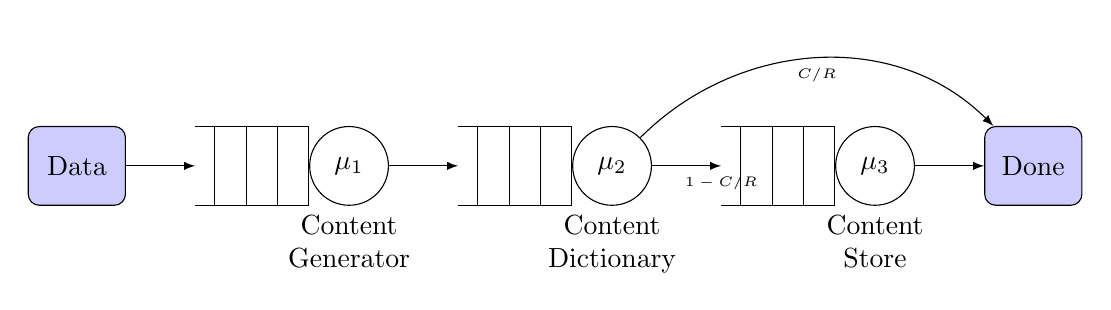
\begin{tikzpicture}[start chain=going right,>=latex,node distance=0pt]
\node[
  block,
  minimum height=1cm,
  text width=1cm,
  on chain
  ] (data) {Data};

\node[
  node distance = 25pt,
  rectangle split, 
  rectangle split parts=4,
  draw, 
  rectangle split horizontal,
  text height=0.5cm,
  text depth=0.5cm,
  on chain,
  inner ysep=0pt] (cgq) {};
\fill[white] ([xshift=-\pgflinewidth,yshift=-\pgflinewidth]cgq.north west) rectangle ([xshift=-15pt,yshift=\pgflinewidth]cgq.south);
\node[draw,circle,on chain,minimum size=1cm] (cgs) {$\mu_1$};

\node[
  node distance = 25pt,
  rectangle split, 
  rectangle split parts=4,
  draw, 
  rectangle split horizontal,
  text height=0.5cm,
  text depth=0.5cm,
  on chain,
  inner ysep=0pt] (cdq) {};
\fill[white] ([xshift=-\pgflinewidth,yshift=-\pgflinewidth]cdq.north west) rectangle ([xshift=-15pt,yshift=\pgflinewidth]cdq.south);
\node[draw,circle,on chain,minimum size=1cm] (cds) {$\mu_2$};

\node[
  node distance = 25pt,
  rectangle split, 
  rectangle split parts=4,
  draw, 
  rectangle split horizontal,
  text height=0.5cm,
  text depth=0.5cm,
  on chain,
  inner ysep=0pt] (csq) {};
\fill[white] ([xshift=-\pgflinewidth,yshift=-\pgflinewidth]csq.north west) rectangle ([xshift=-15pt,yshift=\pgflinewidth]csq.south);
\node[draw,circle,on chain,minimum size=1cm] (css) {$\mu_3$};

\node[
  node distance = 25pt,
  block,
  minimum height=1cm,
  text width=1cm,
  on chain
  ] (done) {Done};

\draw[->] (cgs.east) -- (cdq.west);
\draw[->] (data.east) -- (cgq.west);
\draw[->] (cds.east) -- (csq.west) node[align=center, below] {\tiny$1-C/R$};
\draw[->] (css.east) -- (done.west); 
\path[->] (cds) edge[out=45, in=135] node[below]{\tiny$C/R$}(done);

\node[align=center,below] at (cgs.south) {Content \\ Generator};
\node[align=center,below] at (cds.south) {Content \\ Dictionary};
\node[align=center,below] at (css.south) {Content \\ Store};
\end{tikzpicture}

\captionsetup{format=myformat}
\caption{Our simplified deduplication system model. It is essentially 3 server open queuing system. At the content dictionary, C/R of the segments exit the system and 1-C/R of the segments are passed on to content store. All data are assumed to be immediately available at the memory and all three servers have exponentially distributed service time.}
\label{fig:queue}
\end{figure}

%dedup component
The deduplication process itself can be divided into largely three parts as shown in \figurename~\ref{fig:queue}. First part of the process generates a sequence of segments from input data stream which we call the \emph{content generator}. In the second phase, the deduplication system generates a dictionary of segments which is in turn used to identify the duplicate segments which we call the \emph{content dictionary}. In the last phase, new segments are stored on a persistent storage system which we call the \emph{content store}. The later two components form a \emph{content addressable storage}(CAS).

\subsection{Content Generator}
The goal of the content generator is to maximize the redundant segments while minimizing the number of segments generated.
These two goals often conflict with each other since the amount of duplicate data tends to increase with smaller segments size.
This is due to the fact that the generation of segments are typically done in stateless manner to keep up with the huge data size and stringent throughput requirements.
Recent papers try to overcome this limitation through a two level definition of contents~\cite{kruus:2010, bobbarjung:2006}.
However, these approaches come at the extra computation cost and are applicable only when there are less stringent throughput requirements.

%segmentation types
These are the three most common methods to define the segment boundaries also known as the \emph{anchors}~\cite{zhu:2008, muthitacharoen:2001}.
\begin{itemize}
  \item \emph{File based}: A file boundary becomes the segment boundary.
  \item \emph{Size based}: The anchors are designated every $k$ bits which determines the boundaries for the segment. Therefore, any addition or deletion of data results in shifted anchors which is propagated until the end of the data stream. This effect is known as the \emph{boundary shifting problem}~\cite{muthitacharoen:2001}.
  \item \emph{Content based}: An anchor is generated based on the content of the data which becomes the boundaries for the segments. Therefore the anchors are shifted together with the contents in the case of addition and deletion of the data.
\end{itemize}

The \emph{content based} approach is the most popular method used in data deduplication due to the boundary shifting problem found in the size based method.
Average, maximum and/or minimum segment size are usually specified for the content based approach. This allows system to expect segments of the bounded size which makes the segment handling simpler but also ensures that amount of size variation is limited which can cause loss of redundancy~\cite{eshghi:2005}.

%decoupling from the rest of the system
From the system perspective, the content generator is the source generator for the CAS. Typically, any information about the original data stream is lost after this point. This justifies our looking the dataset as a sequence of segments since beyond this point, the system is effectively decoupled from the original dataset.

\subsection{Content Dictionary}
%hash
The content dictionary is typically a hash table which is keyed by hash of segments. Hash functions used typically provide one-way property as well as collision resistance. While only the collision resistance is required for correct functionality, one-way property is also attractive to ensure that the malicious users cannot corrupt the system by generating hash collisions.

For a large dataset, the content store itself becomes significantly large.
To relax the memory requirements for the deduplication system, the content dictionary is typically stored on the disk~\cite{mandagere:2008, lillibridge:2009, zhu:2008, bhagwat:2009} .
Only a portion is cached onto the memory at a time. Furthermore, any writes to the index table must be serialized which require expensive locks~\cite{clements:2009}. Therefore, the caching algorithm for the index table is one of the major performance factor within the deduplication system.

To avoid unnecessary accesses to the index table, Bloom filter~\cite{bloom:1970} is used to quickly determine segments that are not in the index table~\cite{zhu:2008}. While the backup stream typically exhibit an inherent spatial locality between the segment instances~\cite{zhu:2008}, more intelligent caching schemes that uses data similarities have also been proposed~\cite{lillibridge:2009, bhagwat:2009}.

Regardless of caching scheme, it is clear that content dictionary determines the data path for any given segment. While every segment must read the index table at least once, only the new segments result in it's update. Furthermore, these new segments must be passed down to the content store to be store on the disk. Problem is more complicated for the read where segments maybe fragmented in various places both for the actual contents and the dictionary. A recent work duplicated heavily used segments over the physical disk such that the average seek time can be minimized~\cite{koller:2010}. However, such approach assumes small working set of segments and is heavily workload dependent.

In this work we assume nothing about the caching policy of the content dictionary or any other auxiliary data structure to minimize the access to the dictionary. We only assume that the different segment types results in different resource requirements in regular read/write operations.

\subsection{Content Store}

Once the segments are identified as new content that needs to be stored, it is passed down to the content store to be processed. Various different mechanisms are possible. The content may already be on the disk and the content store only generates a logical mapping and freeing of segments~\cite{clements:2009, rhea:2008} or use log-based filesystem to optimize for the in-band writes~\cite{zhu:2008}.

The content store is not affected specifically by the deduplication system. While inherent \emph{copy-on-write} (COW) support of storage subsystem~\cite{bonwick:2003, dillon:2008} allows easier sharing of segments, the fundamental operations of underlying storage does not differ from dataset to dataset. Therefore, we focus mostly on the behaviors of the content dictionary in this paper.


  % deduplication virtualization 
\chapter{Statistical Tools}
\label{TOOL}
\section{Plackett-Burman designs}
\label{BG_PB}
The \emph{Plackett-Burman design} (PB design)~\cite{plackett:1946} minimizes the number of experiments required to estimate the effect of independent variables on the dependent variable. 
Basically, it estimates the effect of single input parameter on an output in such a way that variance of this effect due to other inputs is minimized. 
The effect is an approximation of the full factorial design but with linear complexity. 
Required assumption is that higher order interaction effects are negligible. 
PB design has been widely used to evaluate effect of benchmark input parameters on processor performance~\cite{yi:2003} and database query processing performance~\cite{debnath:2008}, for example.

Formally, the main effect  $m_1$ of input variable $x_1$ on output $y$ is defined to be 
\begin{equation}
m_1 = \frac{[\sum f(x'_1, x_2, ..., x_n)-\sum f(\overline{x_1}, x_2, ..., x_n)]}{2^n}
\end{equation}
where $x'_1$ represents some extreme value of $x_1$ and $\overline{x_1}$ represents the mean of $x_1$. 
$f$ is an unknown function which maps all $x_i$ to $y$. 
The summation is carried out for all possible combination of $x_2$ through $x_n$. 
Hence, the effect of $x_i$ is simply maximum deviation of $y$ given maximum deviation of $x_i$. 

The goal of PB design is to estimate all $m_i$s such that
\begin{equation}
S=\sum\limits_j (\widehat{y_j}-M-a_{j1}m_1-a_{j2}m_{2}...-a_{jn}m_n+\alpha)^2
\end{equation}
is minimized. 
$\widehat{y_j}$ is simply the sampled value of $y$ at time $j$ and $M$ is mean value of all $y_j$s. 
$a_{ji}$ takes value $\pm 1$ based on whether the $x_i$ had positive or negative effect on $\widehat{y_j}$. 
$\alpha$ is the higher order effects which are ignored based on the observations made by Fisher~\cite{fisher:1936}. 
Since there are $n$ values to be estimated, the minimum number of experiments required to derive a unique set of $m_i$ is $n+1$. 
Plackett and Burman proved that $S$ can indeed be minimized using $\lceil(n+1)/4\rceil*4$ experiments assuming $\alpha = 0$~\cite{plackett:1946}.

\section{Independent Component Analysis}
\label{BG_ICA}
While the PB method quantifies effect of each input parameters to output of interest, it does have one major drawback. 
Because the effect estimation assumes any higher order effects to be zero, the estimated effects of any main factor is partially aliased with any interactions not including that particular main factor. 

In contrast, \emph{Principal Component Analysis} (PCA) and \emph{Independent Component Analysis} (ICA) estimate the effect of uncorrelated components of original factors~\cite{stone:2004}. 
These components may not reflect any intuitively meaningful parameter. 
However, they do provide a uncorrelated set of factors that can be derived from the original ones. 
The limitation of the PCA is that it requires the original factors to be normally distributed. 
ICA is a more generic approach in that such assumption is not required~\cite{christopoulos:2008}. 
It has been observed that ICA performs better than PCA in capturing processor workload space~\cite{eeckhout:2005}. 

In essence, ICA tries to identify statistically independent components from given factors. 

Formally, ICA estimates a matrix $\mathbf{W}$ such that given $\mathbf{x}=(x_1, x_2, ..., x_n)$ with joint \emph{probability density function} (pdf) $p_x(x_1, x_2, ..., x_n)$ such that $\mathbf{y}=\mathbf{W} \times \mathbf{x}$ has joint pdf $p_y(\mathbf{y}$ with following property.
\begin{equation}\label{independence}
E[y_1^{p_1}, y_2^{p_2}, ..., y_m^{p_m}]=E[y_1^{p_1}]E[y_2^{p_2}]...E[y_m^{p_m}]
\end{equation}
for every integer value of $p_i$ and $m \le n$. Equation \ref{independence} is the definition of independence.

\section{Linear Regression}
\label{LM}

A general model that predicts $P$ given $W$ is:
\begin{equation}
P=f_P(w_1, w_2, w_3, ...) +\epsilon
\end{equation}
where $w_i$'s are set of controlled variables and $P$ is metric of
interest. Estimating function $f_P$ without any assumption is
computationally expensive if not impossible. Therefore, we restrict
the form of $f_P$ to a generic linear model of the form:
\begin{equation}\label{lm}
\begin{split}
P=\beta_0+\beta_1 w_1+\beta_2 w_2+...+\epsilon=W\beta+\epsilon\\
W=\begin{bmatrix}1 & w_1 & w_2 & w_3 & ... \end{bmatrix},\;
\beta=\begin{bmatrix}\beta_0 \\ \beta_1 \\ \beta_2 \\ ... \end{bmatrix}
\end{split}
\end{equation}
One thing to note here is that the linear model only dictates how the
$\beta$ values interact with the controlled variables. The controlled
variables themselves can be in the form of any scale. This means that
contrary to what many believe, $W$ does not need to have linear
relationships with $P$. The goal is to estimate $\beta$ such
that $\epsilon$ is acceptable. Typically, we assume that the effects
of any factors not being modeled result in white noise and that the
$\epsilon$ should be normally distributed.

\section{Analysis of Variance(ANOVA)}

\emph{ANOVA} is a widely used technique to separate the total
variation ($\mathit{SST}$) in a set of measurements into a component
due to random fluctuations ($\mathit{SSE}$) and a component due to
actual difference among the alternatives
($\mathit{SSA}$)~\cite{lilja:2005}.

Intuitively, we can assume that the size of the actual component is
$0$ and calculate the probability of this assumption being true.
If the assumption is highly unlikely to be true than we can reject
this assumption. This assumption is typically called the \emph{null
  hypothesis} and the procedure is called \emph{hypothesis testing}.
Given $n$ experiments for each of $k$ alternatives, total variation is
sum of squares of difference between each of $n*k$ experiments and
overall mean, $\overline{y}$. Similarly, the variation due to the
effects of the alternatives is the sum of squares of the differences
between the mean of the measurements for each alternatives and overall
mean. Lastly, the variation due to errors is the sum of the squares
of the differences between the individual measurements and the mean of
all measurements for a particular alternative, $\overline{y_j}$.
\begin{align}
\overline{y_j}&=\frac{\sum_{i=1}^ny_{ij}}{n}\\
\overline{y}&=\frac{\sum_{j=1}^k\sum_{i=1}^ny_{ij}}{kn}\\
\mathit{SSA}&=n\sum\limits_{j=1}^k(\overline{y_j}-\overline{y})^2\\
\mathit{SSE}&=\sum\limits_{j=1}^k\sum\limits_{i=1}^n(y_{ij}-\overline{y_j})^2\\
\mathit{SST}&=\sum\limits_{j=1}^k\sum\limits_{i=1}^n(y_{ij}-\overline{y})^2\\
           &=\mathit{SSA}+\mathit{SSE}
\end{align}

To test if $\mathit{SSA}$ is statistically significant, we use
\emph{F-test}. We can say that $\mathit{SSA}$ is significantly higher
than $\mathit{SSE}$ at $\alpha$ level significance if the calculated
\emph{F-statistic} is larger than the \emph{critical F value},
$F_{[1-\alpha;(k-1),k(n-1)]}$. Note that $k-1$ is the degree of
freedom for $\mathit{SSA}$ and $k(n-1)$ is the degree of freedom for
$\mathit{SSE}$. We can calculate \emph{F-statistic} of the experiment
by:
\begin{equation}
\begin{split}
\textit{F-statistics}&=\frac{\mathit{SSA}(k(n-1))}{\mathit{SSE}(k-1)}\\
 &=S_a^2/S_e^2
\end{split}
\end{equation}
where $S_a^2$ is the variance of $\mathit{SSA}$ and $S_e^2$ is the
variance of $\mathit{SSE}$. Therefore, F-statistic is nothing but a ratio of the signal variance and the noise variance. \emph{Critical F values} defines the minimum required ratio for the signal to have a statistical significance.
\emph{Critical F values} for a given confidence are tabulated in numerous literature~\cite{lilja:2005}.

A more compact representation of the same information is the
\emph{p-value} which is defined to be
\begin{equation}
p=1-P(F\le f)
\end{equation}
where $P(F \le f)$ can be found from \emph{F-density function} which can
be found in numerours statistics text books~\cite{lilja:2005}.
\emph{P-value} represents the probability that $SSA$ is not statistically
significant which is typically rejected if the \emph{p-value} is less
than 0.05.

\nohhyun{pca, simualted anealing, k-mean clustering, arima}
       % sampling virtualization anova 
\chapter{Storage Benchmark Programs}
\label{BENCH}

%%The reason storage benchmarking is difficult and what we want to do.
Storage system performance is one of the most critical factors in meeting overall system performance expectations. 
The performance variances of typical storage systems today can vary by orders of magnitude~\cite{chen:1993}. 
It is very easy to get misled by the performance numbers without understanding the relationship between the storage workload and its performance variances. 

Characterizing the workload for storage systems is typically much more complex than it is for the processors. 
In a simple uni-processor case, it is possible to calculate metrics such as instruction per cycle based on the various cache misses, mis-predictions and number of instructions. 
However, storage systems typically have a much more state-dependent responses. 
For example, a cache miss does not always result in the same penalty, and the service time for a given request depends not only on the  current request but also on all requests in the queue as well as the layout of the data. 
Therefore, two very similar workloads may perform very differently since the small differences could force the state transition path into completely different directions. 
For example, current layout of the data could force a sequential write to become fragmented. 
This then cause the sequential read of the same data to be slow. 
This in turn has effect on any requests that are scheduled after it within the request buffer.

We evaluated current storage benchmarking tools and analyze the effects of different parameter settings on various performance metrics. 
Based on the experiments, we quantify the effects of various parameters for three benchmarks. 
In addition, we also evaluate which parameters are needed to effectively cover the entire storage system performance space and we propose a new benchmark tool based on our evaluation.

\section{Limitations of Current Approach}
The best method for benchmarking a storage system would be to deploy the system under test in the real environment and look at the execution time of the processes that will be run. 
Obviously this approach is too costly to evaluate various feature and performance enhancements. 
Therefore, system architects and designers resort to either a set of traces collected from a real system or a set of synthetic benchmarks.

The problem with using a real trace is that there is no way to determine the coverage of the workload space. 
For example, a given Exchange server trace may perform very well on system A. 
However, it is difficult to determine if system A will perform as well for all Exchange servers. 
Furthermore, it is impossible even to provide any range of potential performances with a single trace. 
As mentioned above, a small change in the trace could result in a very different performance results.

Numerous synthetic benchmarks have been proposed over last few decades. 
The major benefit of these benchmarks is that they allow you to change the characteristics of the workload in a quantitative manner. 
However, current benchmarks either provide numerous parameters to set without providing any insights to the importance of each parameter~\cite{axboe:2008, vandenbergh:2008, katcher:1997, wolman:1989, norcott:2006, coker:2001} or they provide a representative set of parameters that claim to represent a wide range of applications. 
When there are numerous parameters to set, users typically test a few set of ad hoc settings based on their experience which does not always  result in an accurate representation of real workloads. 

\section{Benchmark Programs under Test}
As a proof of concept, we evaluate two different benchmarks tools, PostMark~\cite{katcher:1997} and FIO~\cite{axboe:2008}.

Typically, the evaluated systems are only tested on single configuration of a given benchmark. 
This is problematic since system A may perform better than system B for one configuration of the benchmark but not the others. 
It is critical to either define when the system A performs better or show that system A performs better B in wide range of workloads by testing with multiple configurations that provide wide coverage. 

\subsection{PostMark}
\begin{table}
\centering
\begin{tabularx}{0.9\textwidth}{
  X | 
  >{\centering}X 
  >{\centering\arraybackslash}X
}
\hline
\bfseries Name        &\bfseries Level Low  &\bfseries Level High     \\
\hline\hline
min\_file\_size       &512B                 &4KiB                     \\
max\_file\_size       &4KiB                 &16MiB                    \\
init\_file\_count     &1000                 &10000                    \\
transaction\_count    &10000                &100000                   \\
read\_size            &512B                 &32KiB                    \\
write\_size           &512B                 &32KiB                    \\
file\_system\_buffer  &false                &true                     \\
read\_append\_ratio   &1:9                  &9:1                      \\
create\_delete\_ratio &5:5                  &9:1                      \\
directory\_count      &1                    &1000                     \\
\hline
\end{tabularx}
\captionsetup{format=myformat}
\caption{PostMark input parameters and input levels assigned to each parameter.}
\label{pm_param_t}
\end{table}
  
PostMark was designed for filesystem benchmarking with specific interest to performance of handling small file accesses in Internet software~\cite{katcher:1997}. 
It provides 10 different parameter settings shown in \tablename~\ref{pm_param_t} together with their level settings. 
Most of level decisions were straight forward except the \emph{create\_delete\_ratio}. 
Initially, we set the low bound to be 1:9 where 10\% of the operations are create and 90\% deletion. 
However, we soon realized that the bound is too unrealistic. 
If the deletion of file happens more than the creation, the system will soon become empty of files. 
Therefore, we set the low bound to be 50\% where the creation and deletion is equally like to occur. 

Aside from these, it also provide two more benchmarking parameter for setting the random variable seed and controlling result format. 
The \emph{transaction\_count} only controls the duration of the run and not the arrival rate or the IO depth. 
Therefore, it is also a benchmark parameter. 
The \emph{file\_system\_buffer} parameter is a system parameter which is forces all writes to bypass the filesystem buffer.

PostMark lacks control over arrival pattern and does not support sequential access pattern. 
Since these two characteristics play a major role in how the storage system performs, we can guess that the coverage of PostMark will not be great. 
Also, Postmark does not perform any overwrites which suggest that Postmark is unsuitable for evaluating storage systems where overwrites are expensive such as SSDs.
 
Postmark reports seven performance metrics, \emph{transaction per second} (tps), create tps, read tps, append tps, delete tps, read throughput and write throughput. 
 
\subsection{Flexible IO Tester (FIO)}
\begin{table}
\centering
\begin{tabularx}{0.9\textwidth}{
  X | 
  >{\centering}X 
  >{\centering\arraybackslash}X
}
\hline
\bfseries Name      &\bfseries Level Low  &\bfseries Level High     \\
\hline\hline
operation           &read                 &write                    \\
access\_pattern     &sequential           &random                   \\
files\_used         &1                    &100                      \\
min\_file\_size     &512B                 &1MiB                     \\
max\_file\_size     &1MiB                 &1GiB                     \\
min\_block\_size    &512                  &4KiB                     \\
max\_block\_size    &4KiB                 &64KiB                    \\
io\_depth           &1                    &100                      \\
overwrite           &false                &true                     \\
fsync               &false                &true                     \\
thinktime           &0us                  &1000us                   \\
write\_buffer\_sync &false                &true                     \\
file\_service       &roundrobin           &random                   \\
thread\_count       &1                    &8                        \\
threads\_similarity &false                &true                     \\
posix\_fadvise      &false                &true                     \\
async\_io\_engine   &false                &true                     \\
io\_engine\_queue   &false                &true                     \\
directio            &false                &true                     \\
buffer\_alloc       &malloc               &mmap                     \\
\hline
\end{tabularx}
\captionsetup{format=myformat}
\caption{FIO input parameters and input levels assigned to each parameter.}
\label{fio_param_t}
\end{table}

FIO was designed for benchmarking as well as stress/hardware verification~\cite{axboe:2008}. 
It works directly on block devices as well as files. 
In this experiment, we tested it on files for the sake of consistency with PostMark.

FIO has over 30 different input parameters. 
However, some of those parameters are completely dependent on other parameters and was discarded. 
Also, some of the parameters, when set, caused bus errors on the system we tested. 
As a result, we extracted 20 input parameters as shown in \tablename~\ref{fio_param_t}. 
Every experiment was run for 10 minutes., which was sufficient to ensure that the system reached a steady state. 

FIO can generate multiple independent streams of requests. 
In this study, we evaluate the effect of multiple streams as function of two parameters, \emph{thread\_count} and \emph{threads\_similarity}. 
The thread\_count parameter is self-explanatory. 
When the thread\_similarity is true, we generate either set of very similar streams with only difference being the random seed. 
When it is false, we generate threads that are at maximum distances from each other in the parameter space. 
This can be achieved by choosing different experiments within PB design.

FIO also allows you to control number of outstanding requests controlled by \emph{io\_depth}. 
The \emph{posix\_fadvise} option allows to you enable file advisory information to the operating system~\cite{plonka:2007}. 
FIO provides 13 different types of IO engines. 
Some of them did not work on our system but we use 4 based on the two characteristics of the IO engines, synchronous/asynchronous and multiple/single buffer.

FIO provides a detailed distribution of performance measurements as well as aggregated numbers. 
In our study, we use 4 metrics, read throughput, write throughput, average read latency and average write latency. 
These metrics were chosen not only because they are important performance metrics but also so that the results can be compared against PostMark for out coverage analysis. 
For the experiments with more than 1 thread, the throughputs are simply added and the latency is averaged.

\section{Quantative Analysis}

\subsection{Experiment Flow}
 The experiment is designed to evaluate the effect of various parameters of different benchmarks and coverage of each benchmark. 
We first use PB design to evaluate the effect of each parameter with minimum number of experiments.  
Once the effect has been calculated, we perform ICA on the performance results from each benchmark to estimate equal number of independent components. 
These components are clustered to generate a view of coverage of each benchmark.
 
 This lets us analyze what are the key parameters and whether both benchmarks are needed for a through evaluation of storage systems.

\subsubsection{Evaluation of Benchmark Parameter Effect}

\begin{figure}[!t]
\centering
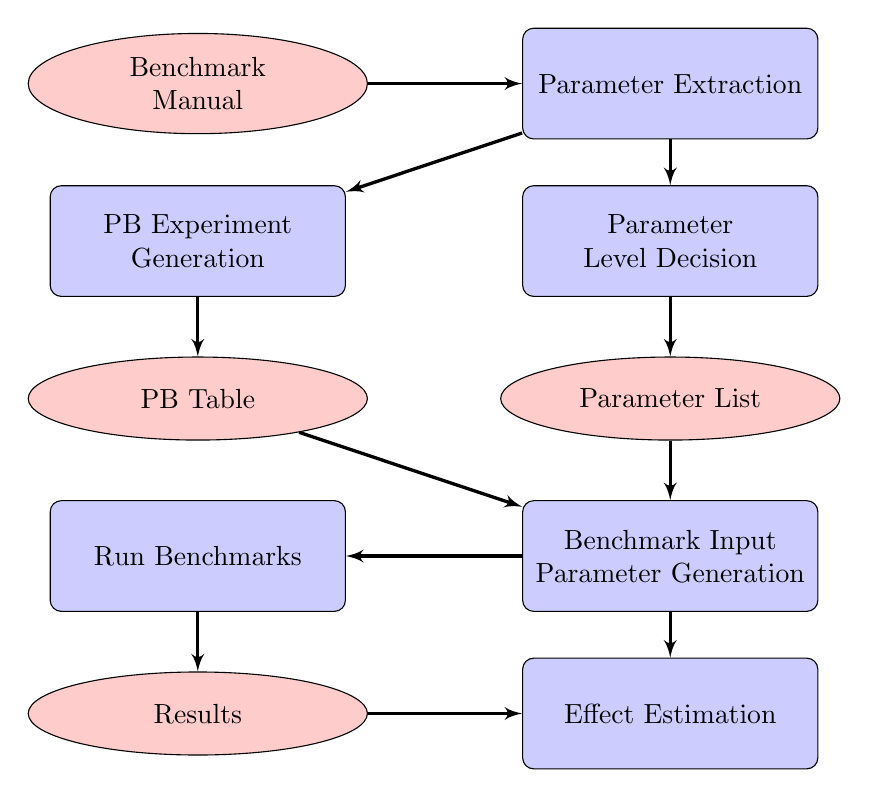
\begin{tikzpicture}[auto,node distance=2cm]
    % Place nodes
    \node [block, node distance=4cm] (init) {Parameter Extraction};
    \node [cloud, left of=init, node distance=6cm] (manual) {Benchmark Manual};
    \node [block, below of=init] (lvl) {Parameter Level Decision};
    \node [block, below of=manual] (PB) {PB Experiment Generation};
    \node [cloud, below of=lvl] (p_list) {Parameter List};
    \node [cloud, below of=PB] (PB_table) {PB Table};
    \node [block, below of=p_list] (input) {Benchmark Input Parameter Generation};
    \node [block, left of=input, node distance=6cm] (run) {Run Benchmarks};
    \node [cloud, below of=run](result){Results};
    \node [block, right of=result, node distance = 6cm](eval){Effect Estimation};
    % Draw edges
    \path [line] (manual) -- (init);
    \path [line] (init) -- (lvl);
    \path [line] (init) -- (PB);
    \path [line] (PB) -- (PB_table);
    \path [line] (lvl) -- (p_list);
    \path [line] (p_list) -- (input);
    \path [line] (PB_table) -- (input);
    \path [line] (input) -- (run);
    \path [line] (run) -- (result);
    \path [line] (result) -- (eval);
    \path [line] (input) -- (eval);
\end{tikzpicture}

\captionsetup{format=myformat}
\caption{Experiment flow for estimating the parameter effects on performance.}
\label{pb_flow_t}
\end{figure}

First, we use PB method to determine the effect of each parameters on each benchmarks seperately. 
The experiment flow for effect estimation is shown in \figurename~\ref{pb_flow_t}. 
\emph{Parameter Extraction} phase tries to extract parameters from benchmark documentation in such a way that each parameter can be varied independently of others. 
This is not always easy as shown in the description of the benchmarks. 

For every parameter extracted, a two extreme level values are designated as shown in \tablename~\ref{pm_param_t} and \tablename~\ref{fio_param_t}. 
Also, once the number of parameter is known, the size of PB design is also known which is required to generate PB design table.  
Since the number of parameters for Postmark is 10 and FIO is 22, PB table of size 12 and 24 are used respectively. 
While any Hardamard matrix~\cite{hadamar:1954} can be used, we use the matrices shown in equation \ref {pb12} for 11 factor experiment.  
PB table for 23 factors can be found in Plackett and Burman's original paper~\cite{plackett:1946} and we omit it due to the space constraint. 

\begin{equation}\label{pb12}
\mathbf{PB}(12)=
\left [ {\begin{array}{r r r r r r r r r r r}
  1&  1& -1&  1&  1&  1& -1& -1& -1&  1& -1\\
 -1&  1&  1& -1&  1&  1&  1& -1& -1& -1&  1\\
  1& -1&  1&  1& -1&  1&  1&  1& -1& -1& -1\\
 -1&  1& -1&  1&  1& -1&  1&  1&  1& -1& -1\\
 -1& -1&  1& -1&  1&  1& -1&  1&  1&  1& -1\\
 -1& -1& -1&  1& -1&  1&  1& -1&  1&  1&  1\\
  1& -1& -1& -1&  1& -1&  1&  1& -1&  1&  1\\
  1&  1& -1& -1& -1&  1& -1&  1&  1& -1&  1\\
  1&  1&  1& -1& -1& -1&  1& -1&  1&  1& -1\\
 -1&  1&  1&  1& -1& -1& -1&  1& -1&  1&  1\\
  1& -1&  1&  1&  1& -1& -1& -1&  1& -1&  1\\
 -1& -1& -1& -1& -1& -1& -1& -1& -1& -1& -1\\
\end{array}} \right ] 
\end{equation}

Each row of the PB table represents an experiment and columns represent parameters. 
$-1$ value represents a \emph{low level} while $1$ represents a \emph{high level}. 
It should be noted that not every column can be assigned a parameter. 
You can leave any of the columns out for actual run of the experiments. 
However, it is important to ignore the effect of the unused column later. 

The number of experiment required in equivalent to the number of row of the matrix. 
Every experiment is repeated three times and mean is used to calculate the effect. 
Given $n$ experiment result $\mathbf{y}$, the effect, $e$, of a parameter represented by column $i$ of PB matrix is simply calculated by
\begin{equation}
e=\frac{\mathbf{PB}_i \cdot \mathbf{y}}{\sum \limits_i (\mathbf{PB}_i \cdot \mathbf{y})}.
\end{equation}
Here the denominator is a simple normalization factor to ensure that sum of all effects is 1. 

\subsubsection{Evaluations of Benchmark Coverage}

We use R JADE package~\cite{ilmonen:2010} to generate 2, 4, 8 independent components from the input parameters and the read and the write throughput measured from each benchmark. 
Since the read and the write throughputs are the only common metrics reported from the two benchmarks, only they can be directly compared. 

Once components are estimated, we evaluate the Euclidean distances between all components which corresponds to a single performance metric are calculated. 
Based on the distance, the components are clustered. 
The number of clusters to be used were estimated using dendrograms~\cite{szekely:2005}. 

We evaluate the best number of components for clean clustering and determine the coverage of each benchmark on two performance metrics.  

\section{Results}

\subsection{Effects}
\begin{figure}[!t]
\centering
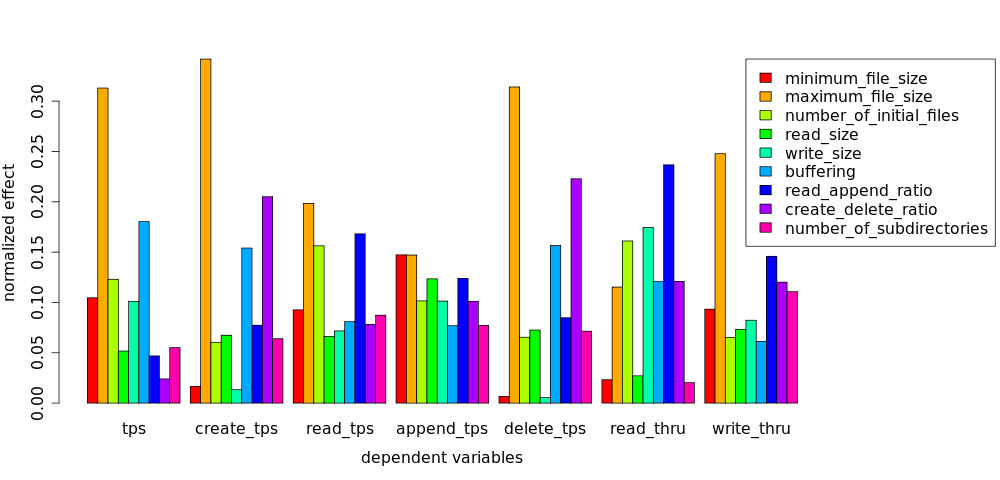
\includegraphics[width=0.9\textwidth]{figure/pm_effect.png}
\captionsetup{format=myformat}
\caption{PostMark parameter effects. 
You can see that some parameters have high effect on a particular kind of performance matric while some have high effect on almost all performance matrics.}
\label{pm_effect}
\end{figure}

\begin{figure}[!t]
\centering
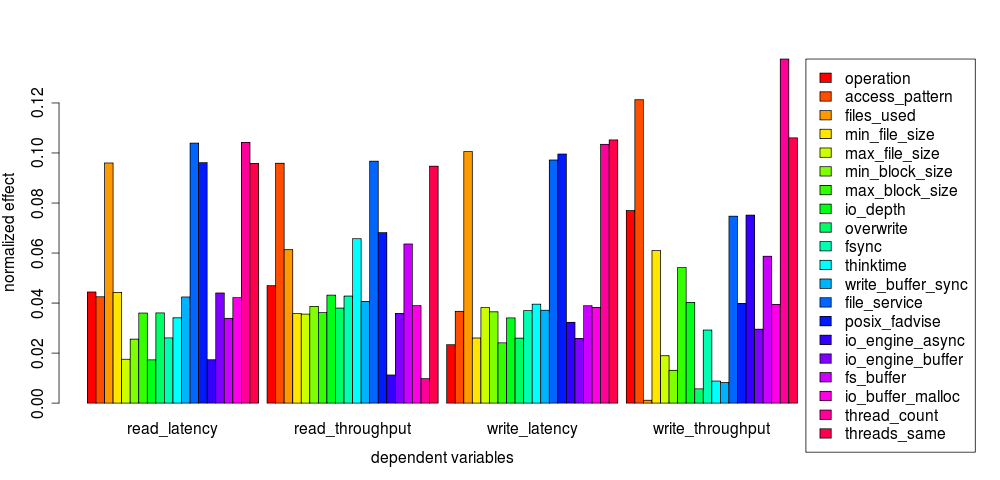
\includegraphics[width=0.9\textwidth]{figure/fio_effect.png}
\captionsetup{format=myformat}
\caption{FIO parameter effects. 
Effect of application threading is the most pronounced in this bechmark. 
However, it will be shown later that the effect of threading can be triggered by other paramters as well.}
\label{fio_effect}
\end{figure}

\figurename~\ref{pm_effect} shows effect of each parameter on each performance metrics reported by Postmark. 
The \emph{maximum\_file\_ size} and \emph{buffering} are the clearly two most important factor in deciding the overall tps. 
The \emph{buffering} parameter controls whether file system buffer should be bypassed using direct IO and the importance of the parameter is obvious. 
However, the effect of the \emph{maximum\_file\_ size} is less obvious. 
Potentially, the high effect is due to the fact that larger file sizes allow a room for longer sequential accesses while the small file sizes force overall access pattern to behave in a more random fashion. 

You can also see that different performance metrics are effected differently. 
The \emph{create\_delete\_ratio} is clearly and obviously important for create tps and delete tps while for append tps, file sizes are more important. 
Another interesting to note is that while read throughput is affected the most by the \emph{read\_append\_ratio}, the write throughput is much more impacted by the file size.

Table \ref{pm_50_t} shows list of parameters with the most effect on each performance metric such that sum of the effects exceed 50\%of overall effects. 
It is shown that roughly 50\% of the all performance variances can be captured using just 2-4 parameters. 
For example, three parameters, \emph{maximum\_file\_size}, \emph{number\_of\_initial\_files} and \emph{buffering}, contribute to 61\% of overall tps variation observed. 
This equate to 4 to 16 experiments for exhaustive evaluation. 
This is a huge improvements over 2048 experiments required for original 12 parameters. 
Furthermore, it is clear that different input combinations must be tested for each performance metric which must be taken into consideration when benchmarking storage systems. 

\begin{table}[!t]
\centering
\begin{tabularx}{0.9\textwidth}{
  l | 
  X 
  c
}
\hline
\bfseries Performance Metric   &\bfseries Parameters           &\bfseries Total Effect  \\
\hline\hline
tps           & maximum\_file\_size                             &0.6164   \\
              & number\_of\_initial\_files                      &         \\
              & filesystem\_buffer                              &         \\
\hline
create\_tps   & maximum\_file\_size                             &0.5469   \\
              & create\_delete\_ratio                           &         \\
\hline
read\_tps     & maximum\_file\_size                             &0.5229   \\
              & number\_of\_initial\_files                      &         \\
              & read\_append\_ratio                             &         \\
\hline
append\_tps   & minimum\_file\_size                             &0.5418   \\
              & maximum\_file\_size                             &         \\
              & read\_size                                      &         \\
              & read\_append\_ratio                             &         \\
\hline
delete\_tps   & maximum\_file\_size                             &0.5369   \\
              & create\_append\_ratio                           &         \\
\hline
read\_thru    & number\_of\_initial\_files                      &0.5722   \\
              & write\_size                                     &         \\
              & read\_append\_ratio                             &         \\
\hline
write\_thru   & maximum\_file\_size                             &0.5137   \\
              & read\_append\_ratio                             &         \\
              & create\_delete\_ratio                           &         \\
\hline
\end{tabularx}
\captionsetup{format=myformat}
\caption{PostMark input parameters required to cover at least 50\% of overall effect for each performance metrics reported.
The maximum number of parameters required does not exceed 4.}
\label{pm_50_t}
\end{table}

\begin{table}[!t]
\centering
\begin{tabularx}{0.9\textwidth}{
  l | 
  X 
  c
}
\hline
\bfseries Performance Metric &\bfseries Parameters &\bfseries Total Effect\\
\hline\hline
read\_latency       & files\_used                               &0.5406   \\
                    & file\_service                             &         \\ 
                    & posix\_fadvise                            &         \\ 
                    & thread\_count                             &         \\
                    & threads\_same                             &         \\
\hline
read\_throughput    & access\_pattern                           &0.5462   \\
                    & write\_buffer\_sync                       &         \\
                    & threads\_same                             &         \\
\hline
write\_latency      & files\_used                               &0.5060   \\
                    & file\_service                             &         \\
                    & posix\_fadvise                            &         \\
                    & thread\_count                             &         \\
                    & threads\_same                             &         \\
\hline
write\_throughput   & access\_pattern                           &0.5170   \\  
                    & thread\_count                             &         \\ 
                    & threads\_same                             &         \\
\hline
\end{tabularx}
\captionsetup{format=myformat}
\caption{FIO input parameters required to cover at least 50\% of overall effect of each performance metrics reported.
The maximum number of parameters required does not exceed 5.}
\label{fio_50_t}
\end{table}

\figurename~\ref{fio_effect} shows the effect of each parameter on four performance metrics measured and \tablename~\ref{fio_50_t} shows list of parameters with the most effect on each performance metric such that sum of the effects exceed 50\%of overall effects. It is interesting to note that the most important parameters for read and write latencies are the same. We can assume that read and write operations themselves do not affect the latency in our system. This can expected, since on HDD, read and write operations do not result in significantly different response time.  Furthermore, we see that the \emph{threads\_same} parameter is important for all metrics. This indicates that the interference between the threads can seriously affect the performance. While the \emph{thread\_count} parameter is also important, the effect on the read throughput is shown to be negligible. Both throughputs are sensitive to the \emph{access\_pattern} which is expected but surprisingly the latency is not. Instead, they are much more sensitive to the \emph{posix\_fadvise} setting. This suggests that latency is not determined by the seek time but rather cache miss penalties. 

\subsection{Coverage of Benchmarks}


\begin{figure}[!t]
\centering
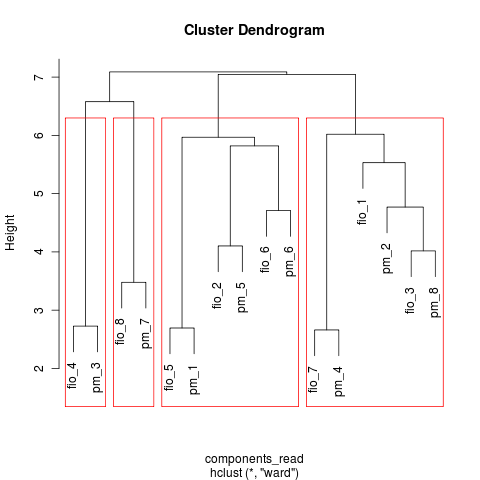
\includegraphics[width=0.8\textwidth]{figure/Rplot001.png}
\captionsetup{format=myformat}
\caption{Read performance coverage of of independent components of PostMark and FIO.}
\label{read_cov}
\end{figure}

\begin{figure}[!t]
\centering
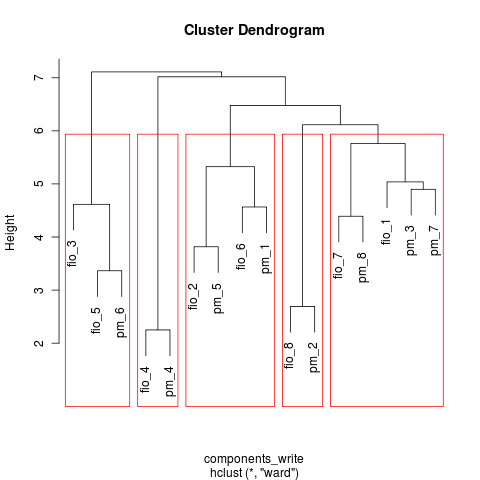
\includegraphics[width=0.8\textwidth]{figure/Rplot002.png}
\captionsetup{format=myformat}
\caption{Write performance coverage of of independent components of PostMark and FIO.}
\label{write_cov}
\end{figure}

The distance between the independent components as well as their clustering is shown in \figurename~\ref{read_cov} and \figurename~\ref{write_cov}. 
In these graphs, each leaf node represents an independent component. 
Since the independent components have no physical meaning associated with them, we number them from 1 to 8 per benchmark. 
We only show the results of 8 components for the brevity. The closer the leaves are on the tree, more similar effect they have on the result. The \emph{height} represents the difference between the subtrees. therefore, evenly spread out components of both benchmark on x-axis suggest similar coverage, while the height of the tree suggest the granularity of the coverage. For example, the FIO component 4 and PostMark component 3 have the similar effect on the read throughput based on the \figurename~\ref{read_cov}. At the same time, FIO component 8 and PostMark component 7 also have similar effect. However, there is a large gap between the two sets of components which are not covered by any of the components as suggested by the \emph{height} of the edges connecting the two subtrees.

An interesting observation is that for read throughput, FIO and Postmark have roughly the same coverage. This is interesting since PostMark have far fewer parameters. It can be concluded if the metric of interest is read throughput, than it does not matter which benchmark you use as long as you can test the key parameters thoroughly.

For the write throughput, FIO does provide wider coverage to the left with component 3, while PostMark provide wider coverage on the right with component 3 and 7. We can safely conclude that each benchmark provide one of more input parameters that affect the write throughput that is not provided by the other benchmark. 

The input parameters that affect the read and write throughput performance shows some difference. They all depend on the size of the files, number of files and mix of operations. However, write throughput is also dependent on file creation and deletion which are not taken into account in FIO. Conversely, PostMark does not consider the number of threads which is another important factor provided by FIO. 

We believe that a good benchmark should have all those components as inputs to provide a wider coverage. 

\section{Conclusion}
Clearly, any storage performance evaluation should consider the effect of critical input parameters that has been described in this paper. We recommend that at least the critical parameters shown in \tablename~\ref{pm_50_t} and \ref{fio_50_t} should be tested thoroughly to gain an approximate sense of the system's performance variation.

The methodology presented in this paper can be applied to any benchmarking tool with set of input parameters that can be adjusted. The key challenge is deciding the range of each parameter. Once this is done, the entire process can be automated. 

Even if the system is designed for a specific workload, it is still beneficial to follow the methodology described in this paper. Since the characteristics of the actual workload is known, a tighter level bounds can be assigned to each parameter. The resulting effect of the parameters can describe how the system reacts to different parameters and can provide valuable insights to workload-system interactions. 

We also show that different benchmarks can still cover roughly the same performance space if the input parameters are chosen appropriately. We suggest that performing a set of through experiments on a single benchmark provides more accurate description of system performance than running a single experiment on the multiple benchmarks. 

However, it is clear that there are specific performance space that can only be explored with a specific benchmark. Since it is difficult to determine what benchmarks cover how much of the performance space, we propose a new benchmark with following properties.
\begin{itemize}
\item IO benchmark tool should provide maximum coverage of storage system's operational space with minimum parameter settings.  
\item The parameters of benchmarking tools should be as independent as possible.
\item The parameters should be exclusively defined as either the system parameter, the workload parameter or the benchmark parameter. 
\item The target interface which the benchmark is testing needs to be clearly defined. 
\item A minimum validation of results should be handled. (eg. Results that suggest under-utilization of target system such that the performance result does reflect its capability.)
\end{itemize}

With this kind of benchmarking tool, most of the systems can be evaluated with a single benchmark with multiple parameter settings. This tool would allow different researcher and developers to report their performance in a more coherent manner which in turn makes performance comparison and reproducing the result easier. 

As a future work, we plan to conduct a comprehensive analysis of more benchmarks and design a new benchmark that provides a wide coverage with few independent parameters. 

   % storage benchmark
\chapter{Storage Performance Model}
\label{SPM}

\begin{table}[!t]
\centering
\begin{tabularx}{\textwidth}{c|X||c|X}
\hline
$W$     & Workload                      & $M_W$   & Workload Model \\ \hline
$S$     & Data Store                    & $M_S$   & Data Store Model \\ \hline
$P$     & Performance(Latency)          & $M_P$   & Performance Model(Prediction) \\ \hline
$\RAND$ & Random \%                     & $\READ$ & Read \% \\ \hline
$\SIZE$ & IO size                       & $\OIO$  & Outstanding IO \\ \hline
\end{tabularx}
\caption{Variables defined in used to describe \romano Performance Model.}
\label{terminology}
\end{table}

\romano Performance Model predicts the performance of a workload on a given data store. 
Before describing \romano Performance Model in detail we define a few variables in \tablename~\ref{terminology} to help describe our model.

\section{\romano Performance Model Framework}

\begin{figure}[!t]
\centering
\begin{tikzpicture}[node distance = 1.5in, auto, font=\small]
\node[disk] (ds) {Data \\ Store};
\node[block, text width=7em, left of=ds] (tv) {Test \\ Vector};
\node[block, text width=7em, right of=ds] (p) {Stats \\ Collector};
\node[block, text width=7em, below of=ds] (MW) {Workload \\ Model ($M_W$)};
\node[block, text width=7em, below of=p] (MS) {Data Store \\ Model ($M_S$)};
\node[block, text width=7em, below of=tv] (MP) {Performance \\ Model ($M_P$)};
\path[arrow] (tv) -- node{\textcircled{1}}(ds);
\path[arrow] (ds) -- node{\textcircled{2}}(p);
\path[arrow] (p) edge[out=270, in=90] node{\textcircled{3}}(MW);
\path[arrow] (MW) -- node{\textcircled{4}}(MS);
\path[arrow] (MW) -- node{\textcircled{6}}(MP);
\path[arrow] (MS) edge[out=110, in=70] node{\textcircled{6}}(MP);
\path[arrow] (p) edge[out=270, in=0] node{\textcircled{4}, \textcircled{5}}(MS);
\path[arrow] (MS) edge[out=340, in=0, loop] node{\textcircled{5}}(MS);
\end{tikzpicture}

\caption{\romano Performance Model framework.}
\label{rpm}
\end{figure}

\figurename~\ref{rpm} outlines how the \emph{\romano Performance Model} is generated and maintained.
The edges in \figurename~\ref{rpm} represents the following procedure.\
\begin{enumerate}
\item The test vector is run on data stores.
\item Average latencies, $P$, as well as the characteristics of the workload~($\RAND$, $\READ$, $\SIZE$ and $\OIO$) per data store are collected at 20 seconds interval.
\item Workload model is generated by determining which of the workload characteristics and their interactions actually affect $P$.
\item From the workload model and the latencies, the data store model is generated via linear regression.
\item The model is updated periodically based on the new data collected while data stores are active.
\item The performance model is derived from the workload and data store model.
\end{enumerate}
In this section we will describe and justify each step of the process involved in generating the performance model~($M_P$).

\paragraph{The Goal}
A system's performance is mainly determined by the system itself and its workload.
Therefore, there should exist a function, $f_P$, that can map a given data store~($S$) and workload~($W$) onto performance~($P$).
\begin{equation}
P=f_P(S, W)\label{psw}
\end{equation}
We define \emph{IO workloads} to be the set of all possible workloads, $W=\{w_i\}$ and \emph{Performance}, $P$, to be the average IO latency.
However, the dimensions of $S$ and $W$ are too large to be parameterized. Furthermore, even if they were not, deriving an accurate non-linear function $f_P$ is difficult.
Therefore, we assume the form of $f_P$ to be some linear combination shown in Equation~\ref{lm} and fit $S$ and $W$ into $M_S$ and $M_W$ such that $P$ can be approximated.
\begin{equation} \label{rlm}
P = M_W M_S+\epsilon = M_P+\epsilon
\end{equation}
The goal of \emph{\romano Performance Model} is to derive $M_W$ and $M_S$ such that resulting $M_P$ is as close to the actual $P$ as possible.

\paragraph{The Problem}
Since we can measure $P$, we need to determine $M_W$ to solve the Equation~\ref{rlm} for $M_S$.
Once $M_W$ is defined, we can use linear regression to derive $M_S$.
Without the knowledge about the true distribution of $\epsilon$, we assume it to be Gaussian and solve for $M_S$ by:
\begin{equation}\label{msSolve}
({M_W}^TM_W)^{-1}{M_W}^TP = M_S
\end{equation}
Equation~\ref{msSolve} is proven to result in smallest $\epsilon$ if the $\epsilon$ is Gaussian distributed~\cite{hayashi:2000}.
While the true distribution of $\epsilon$ may not be Gaussian, we found the resulting $\epsilon$ small enough to justify the assumption.
Therefore, the problem is finding a good $M_W$ such that $\epsilon$ can be minimized.
There is a practical constraint we must satisfy when solving this problem.
The characteristics of workloads that can be used to derive $M_W$ must be collected from the system at run time without too much overhead.
VMware ESXi 5.0 already collects read ratio~($\READ$), average request size~($\SIZE$) and average number of outstanding IOs~($\OIO$) at 20 seconds granularity~\cite{vmware:2006}.
We implement a mechanism to collect one more characteristic to measure amount of seeks~($\RAND$) since it is well known that randomness of IO has large effect on storage performance.
The problem is now reduced to finding a good $M_W$ from $\RAND$, $\READ$, $\SIZE$ and $\OIO$ such that $\epsilon$ is minimized.

\paragraph{Test Vector}
To investigate how $M_W$ can be derived from $\RAND$, $\READ$, $\SIZE$ and $\OIO$, we first define the space of all possible workloads in terms of those characteristics.
\begin{align}
\mathit{random\%} (\RAND) = \{r|r \in \mathbb{I}, 0\le r \le 100\} \\
\mathit{read\%} (\READ) = \{o|o \in \mathbb{I}, 0\le o \le 100\}\\
\mathit{IOsize} (\SIZE) = \{s|s \in 2^n\mathit{B}, n \in \mathbb{N},  9 \le n \le 19\}\\
\mathit{OutstandingIO} (\OIO) = \{ i|i \in \mathbb{N}, 1\le i\le128 \}
\end{align}
Note that we limited the range of $\OIO$ and $\SIZE$ which is not enforced theoretically.
However, they are typically enforced by the system resource limitations such as buffer size.
While different limits can be used, we believe these to be widely applicable in today's systems.
Another thing to note is that we have only defined the $\READ$ and $\RAND$ within $\mathbb{I}$.
While this may result in loss of resolution, $\READ$ and $\RAND$ are always discrete in practice since there can only be finite number of requests and we assume that the close enough values always result in similar latency.
The size of the entire space is $|\OIO| * |\SIZE| * |\READ| * |\RAND| = 14,363,008$.
If we tested each point in space for 2 minutes, it would take $~54$ years to explore all possible combinations.
Therefore we sample this workload characteristics space such that;
\begin{align}
\RAND=\{0\%, 25\%, 50\%, 75\%, 100\%\}\\
\READ=\{0\%, 25\%, 50\%, 75\%, 100\%\}\\
\SIZE=\{1K, 2K, 4K, 8K, 16K, 32K, 64K\}\\
\OIO=\{1, 2, 4, 8, 16, 32, 64\}
\end{align}
which would require 1600 tests and can be done in a couple of days.
This sampled space is our \emph{test vector}.
The idea of vectorizing a multidimensional continuous space into a single discrete vector is analogous to the way application characteristics are represented in \emph{HBench}~\cite{seltzer:1999}.

The reduction in workload space due to sampling 1600 datapoints results in no significant loss of accuracy in the model.
However, the space is still too large for the modeling to be carried out at low cost on on-line systems.
The sampling technique that would provide a reasonable model with minimum testing is an interesting topic we leave for the future research.

We generate our test vector using Iometer~\cite{sievert:2004}.

\paragraph{Workload Model}
How to describe an IO workload in a generic manner is an open question~\cite{liu:2008, wang:2004, kavalanekar:2008, tarasov:2012}.
Unlike Basil~\cite{gulati:2010} and Pesto~\cite{gulati:2011}, \romano generates a separate $M_W$ for each data store.
While it is tempting to derive $M_W$ in a data store independent manner, we found the resulting performance model~($M_P$) to be neither robust nor accurate.
This is because each data store interacts with the characteristics of the workload in a different manner.
\begin{figure}[!t]
\centering
\subfloat[E1]{\label{fig:E1read}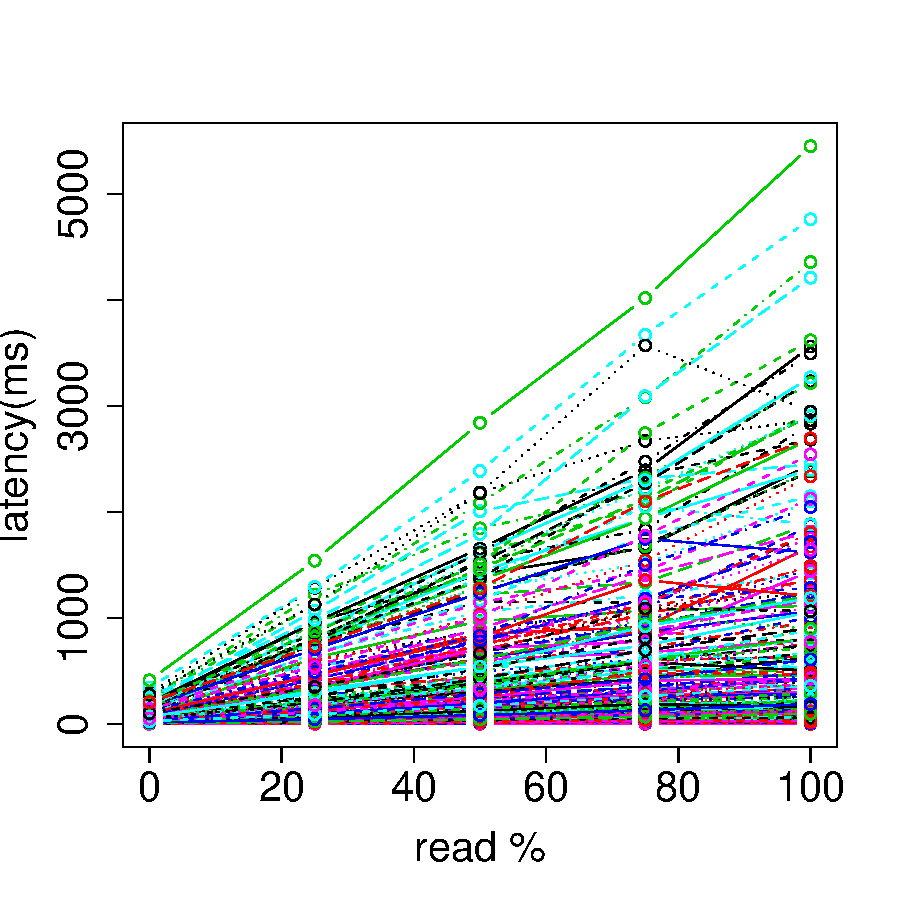
\includegraphics[width=0.5\textwidth]{figure/emc-3disk-raid0_basic_8_120s_read_single_var.pdf}}
\subfloat[N2]{\label{fig:N2read}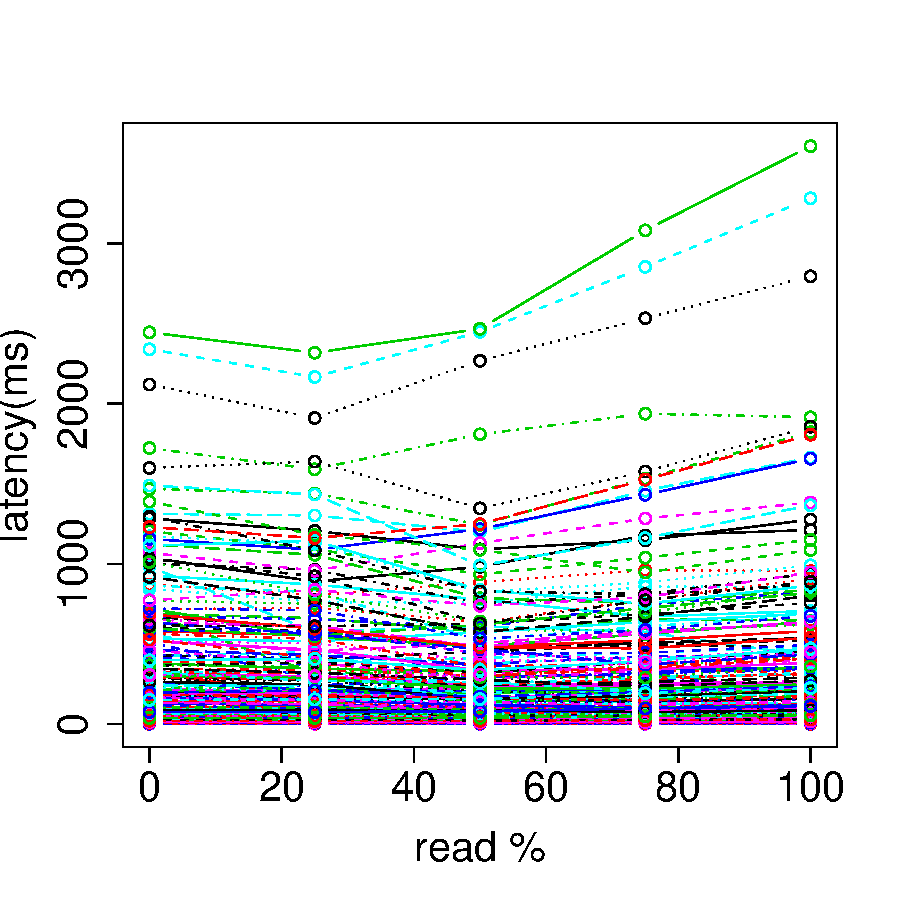
\includegraphics[width=0.5\textwidth]{figure/srs7diskfc_netapp_basic_8_120s_read_single_var.pdf}}
\caption{Effect of \emph{read\%} variation on the \emph{latency} of E1 and N2 data stores.
Each line represent latency~($P$) vs. read\%~($\READ$) while other parameters($\OIO$, $\SIZE$ and $\RAND$) are fixed.
The effect of $\READ$ on E1 is much more predictable(therefore significant) than N2.
}
\label{readParam}
\end{figure}
\begin{table}[!t]
\centering
\begin{tabularx}{\textwidth}{
  X|
  >{\centering} X|
  >{\centering} X|
  >{\centering} X|
  >{\centering\arraybackslash} X
}
\hline
Name    & No. of disks & RAID & Interface & Make \\
\hline
E1  & 3 & 0 & SATA & EMC \\
E2  & 6 & 5 & FC   & EMC \\
N1  & 3 & 5 & SATA & NetApp \\
N2  & 7 & 6 & FC   & NetApp \\
\hline
\end{tabularx}
%\captionsetup{format=myformat}
\caption{Summary of test data stores used in \romano testing.}
\label{ds}
\end{table}
\figurename~\ref{readParam} shows the relationship between $P$ and $\READ$ for two data stores E1 and N2 from \tablename~\ref{ds}.
The plot shows the latency change observed on two different data stores while varying $\READ$ and fixing $\RAND$, $\SIZE$ and $\OIO$.
It is clear that $\READ$ has distinct effect of E1 but not on N2.
This means that $M_W$ for E1 should contain $\READ$ but not N2.
An important thing to note is that the inclusion of $\READ$ in $M_W$ for N2 will result in over-fitting since it is likely to only add to the noise.
Therefore, removing $\READ$ from the workload model actually results in a more robust model that is less sensitive to noise.

Another difficulty arises from the fact that the interactions between the characteristics are significant and cannot be ignored.
While it is possible to use a simple tuple of $\RAND$, $\READ$, $\SIZE$ and $\OIO$, we found the resulting $\epsilon$ to be very large.
Interactions between the characteristics can be factored in by simply adding additional terms for the products of two or more characteristics.
For example, the interaction between $\RAND$ and $\READ$ can be factored in to the model by adding the additional term $\RAND:\READ = \RAND*\READ$.
Therefore, given 4 characteristics, there are $2^4-1=15$ possible terms including the interactions.
To check which of the 15 terms actually have a significant effect on the performance, we conduct ANOVA at 95\% confidence controlling the 15 terms~(using the test vector) and observing the latency on four test data store shown in \tablename~\ref{ds}.

\begin{table}[!t]
\centering
\begin{tabularx}{\textwidth}{
  X|
  >{\centering}X||
  X|
  >{\centering\arraybackslash}X}
\hline
\multicolumn{2}{c||}{E1}  & \multicolumn{2}{c}{E2} \\
\hline
factor        & p-value & factor        & p-value     \\
\hline
\OIO          & 4.83e-06  & \OIO          & $<$ 2e-16   \\
\READ:\OIO        & 3.09e-08  & \RAND:\OIO      & 7.92e-15    \\
\SIZE:\OIO        & 3.45e-03  & \SIZE:\OIO        & $<$ 2e-16   \\
\RAND:\READ:\OIO    & $<$ 2e-16 & \RAND:\READ:\OIO    & $<$ 2e-16   \\
\RAND:\SIZE:\OIO    & 4.51e-03  & \RAND:\SIZE:\OIO    & 3.98e-05    \\
\RAND:\READ:\SIZE:\OIO  & 5.99e-11  & & \\
\hline\hline
\multicolumn{2}{c||}{N1}  & \multicolumn{2}{c}{N2}  \\
\hline
factor        & p-value & factor        & p-value     \\
\hline
\OIO              & 6.85e-03  & \OIO          & 3.06e-16      \\
\RAND:\OIO            & $<$ 2e-16 & \RAND:\OIO        & $<$ 2e-16     \\
\SIZE:\OIO            & $<$ 2e-16 & \SIZE:\OIO        & $<$ 2e-16     \\
\RAND:\READ:\OIO          & 2.33e-05  & \RAND:\READ:\OIO      & 4.68e-08      \\
\RAND:\SIZE:\OIO          & $<$ 2e-16 & \RAND:\READ:\SIZE:\OIO    &   $<$ 2e-16   \\
\RAND:\READ:\SIZE:\OIO        & $<$ 2e-16 &           & \\
\hline
\end{tabularx}
\caption{Result of factorial ANOVA with latency as response and characteristics of workload as the treatment.
Only the factors with p-values less than 0.05 are shown.
%In \romano, these are defined to be the workload model.
%With 95\% probability, these factors have a predictable effect on performance.
}
\label{p_values}
\end{table}
The \emph{p-values} derived from the ANOVA test is shown in \tablename~\ref{p_values}.
These values have a significant effect on performance~($P$) with 95\% confidence.
For example, the $M_W$ for E2 is a row vector of the form;
\begin{equation}
M_W = \begin{bmatrix} \OIO & \RAND*\OIO & \SIZE*\OIO & \RAND*\READ*\OIO & \RAND*\SIZE*\OIO \end{bmatrix}
\end{equation}
The resulting $M_W$ accounts for any interactions as well as their significance on a given data store.
While the cost of the experiment is not cheap, this only has to be done once per data store type in the system.

\paragraph{Data Store Model}
\begin{table}[!t]
\centering
\begin{tabularx}{\textwidth}{
  X|
  >{\centering}X||
  X|
  >{\centering\arraybackslash}X
}
\hline
\multicolumn{2}{c||}{E1}  & \multicolumn{2}{c}{E2}    \\
\hline
factor                & coefficients  & factor            & coefficients  \\
\hline
\OIO                    & 1.064         & \OIO                & 8.370e-01     \\
\READ:\OIO              & 2.828e-02     & \RAND:\OIO        & 6.163e-03     \\
\SIZE:\OIO              & 1.505e-05     & \SIZE:\OIO          & 1.172e-05     \\
\RAND:\READ:\OIO        & 2.277e-03     & \RAND:\READ:\OIO    & 4.079e-04     \\
\RAND:\SIZE:\OIO        & 2.545e-07     & \RAND:\SIZE:\OIO    & 9.970e-08   \\
\RAND:\READ:\SIZE:\OIO  & 9.385e-09     &                   &               \\
\hline\hline
\multicolumn{2}{c||}{N1}  & \multicolumn{2}{c}{N2}          \\
\hline
factor                & coefficients  & factor                & coefficients\\
\hline
\OIO                    & 1.428         & \OIO                    & 1.310\\
\RAND:\OIO            & 1.653e-01     & \RAND:\OIO            & 1.403e-01\\
\SIZE:\OIO              & 1.293e-04     & \SIZE:\OIO              & 9.078e-05\\
\RAND:\READ:\OIO        & -3.24e-04   & \RAND:\READ:\OIO        & 1.579e-06\\
\RAND:\SIZE:\OIO        & 2.052e-06     & \RAND:\READ:\SIZE:\OIO  & 1.514e-08\\
\RAND:\READ:\SIZE:\OIO  & 2.613e-08     &                       & \\
\hline
\end{tabularx}
%\captionsetup{format=myformat}
\caption{Data store model~($M_S$) for four test data stores.
~($M_S$) is a column vector whose entries are shown in the \emph{coefficients} column of the each data store.}
\label{smodel}
\end{table}

Using the $M_W$, we find the $M_S$ using Equation~\ref{msSolve}.
\tablename~\ref{smodel} shows the resulting $M_S$ for the four test data stores.
The \emph{coefficients} columns of each data store form a column vector which is $M_S$ of that data store.
The accuracy of $M_S$ depends heavily on the number of data points.
While initially it can be derived from our test vector, it can be updated from the data collected in production environment to improve its accuracy.
%A great thing about linear regression is that it can also provide a \emph{prediction interval} based on the observed error distribution.

\paragraph{Performance Model}
Finally, we are now ready to calculate $M_P$, which is the prediction of $P$, by taking the cross product of $M_S$ and $M_W$.
One interesting thing to note from \tablename~\ref{p_values} is that all the factors contain $\OIO$.
This is because the average latency~($P$) of all data stores are linear to the number of outstanding IOs~($\OIO$).
Note that it also means that $P$ is not linear to $\RAND$, $\READ$ and $\SIZE$.

We have tested 12 different data stores and verified that the linear relatioship between the outstanding IOs and the latencies hold.
%Let us denote the element of $M_S$ that corresponds to an element of $M_W$ as $M_{S,W}$.
%For example, $M_{S=E1,\OIO}=1.064$ which is the coefficient corresponding to $\OIO$ in \tablename~\ref{smodel} for data store E1.
Therefore, we can rewrite Equation~\ref{msSolve} as;
\begin{equation}\label{rpm:eq}
\begin{split}
M_P&=M_WM_S=M_W'M_S\OIO\\
M_W'&=\frac{M_W}{\OIO}
\end{split}
\end{equation}

Since the \emph{outstanding IO}~($\OIO$) is the number of IO requests outstanding in the queue and $P$ is time the requests spend in the system, by Little's law~\cite{little:1961}, $M_W'M_S$ is the average inter-arrival time of requests.
It is also the average service time of requests at equilibrium and its inverse is the throughput~($T$) in $\mathit{IO}/s$.
Pesto~\cite{gulati:2011} describes the linear relationship between $\OIO$ and $P$ in much more depth and we refer interested readers to their work.

\begin{figure}[!t]
\centering
\subfloat[E1]{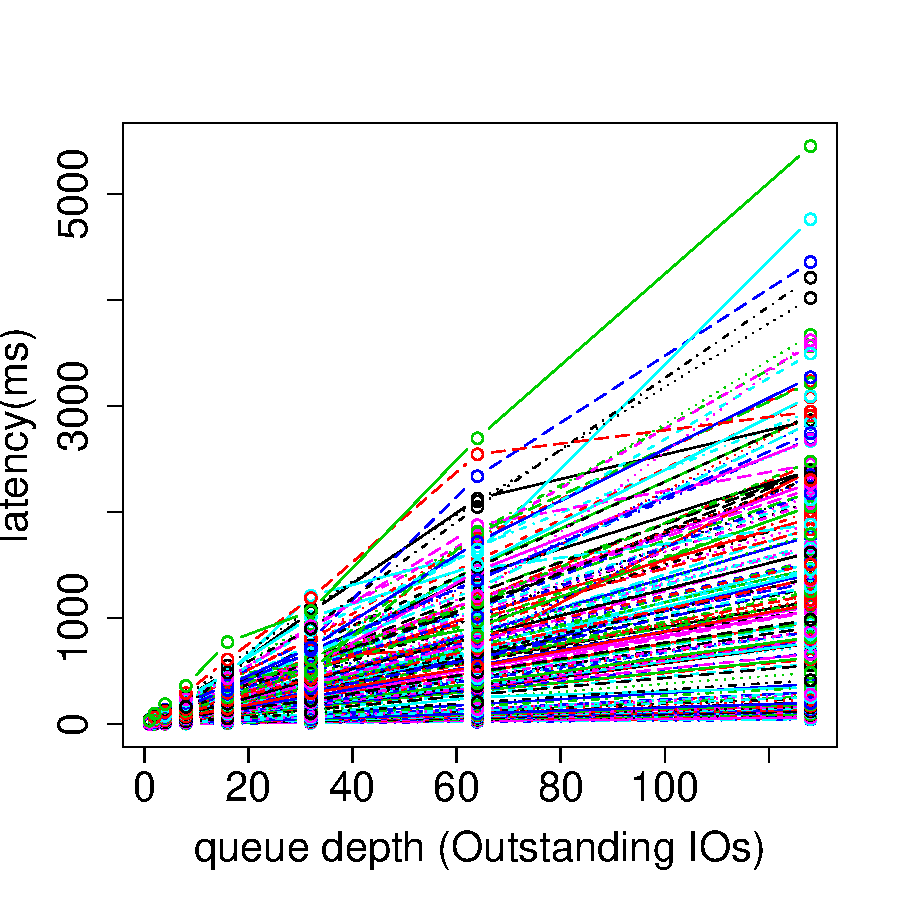
\includegraphics[width=0.5\textwidth]{figure/emc-3disk-raid0_basic_8_120s_oio_single_var.pdf}}
\subfloat[E2]{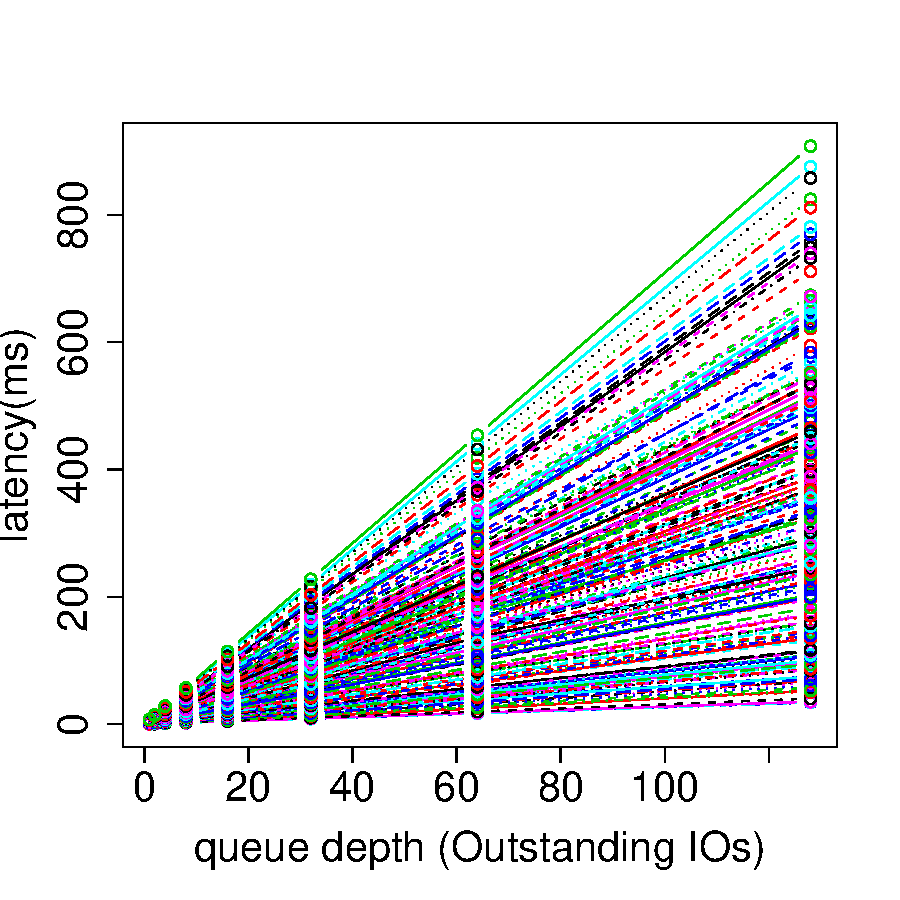
\includegraphics[width=0.5\textwidth]{figure/emc-6diskfc-sp_basic_8_120s_oio_single_var.pdf}}\\
\subfloat[N1]{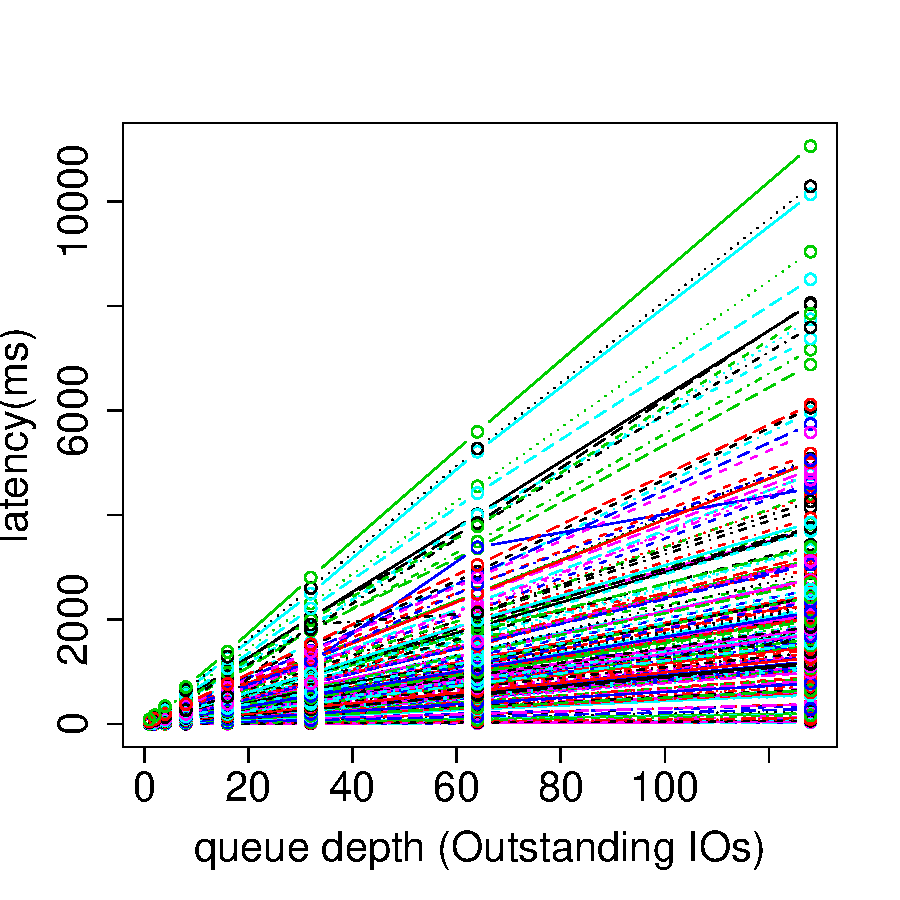
\includegraphics[width=0.5\textwidth]{figure/netapp-3diskata-sp_basic_8_120s_oio_single_var.pdf}}
\subfloat[N2]{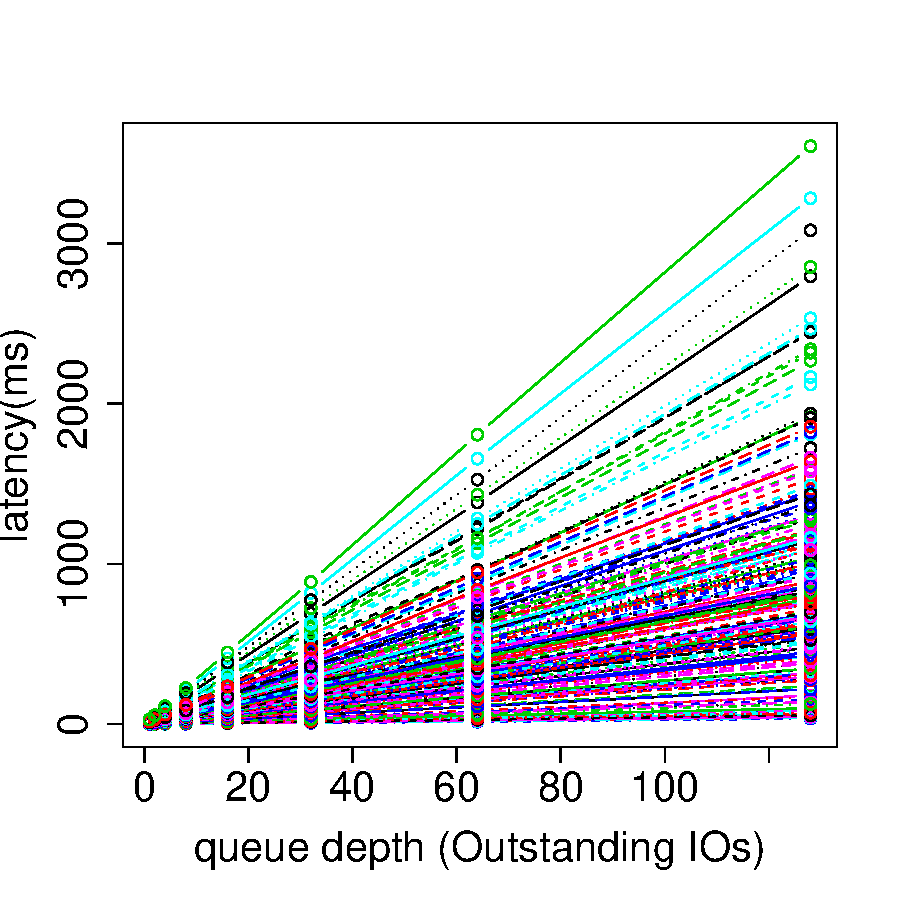
\includegraphics[width=0.5\textwidth]{figure/srs7diskfc_netapp_basic_8_120s_oio_single_var.pdf}}
\caption{Effect of outstanding IO~($\OIO$) variation~(from 1 to 128) on the latency of test data stores.
Each line represent latency~($P$) vs. outstanding IO~($\OIO$) while other parameters are fixed.
Except for the few noise, the relationship is clearly linear for all data stores.
}
\label{oioParam}
\end{figure}
%Simply put, $M_W'M_S'$ is the rate at which the latency increases as more IOs are outstanding at the queue which is constant for all data stores as shown in \figurename~\ref{oioParam}.
The \figurename~\ref{oioParam} shows latency~($P$) change as $\OIO$ is varied while fixing $\RAND$, $\READ$ and $\SIZE$.
Except for some exceptions caused by the measurement errors, all plots show linear relationship between $\OIO$ and $P$.
%Some exceptions are shown which we believe are caused by measurement errors.
$M_W'M_S$ is called \emph{LQ-slope} in Pesto, and we continue to use the terminology for the sake of consistency.
Therefore, we can rewrite Equation~\ref{rpm:eq} to our final form of $M_P$.
\begin{equation}\label{rpmf:eq}
P=M_P+\epsilon=\mathit{LQslope}*\OIO+\epsilon=M_W'M_S\OIO+\epsilon
\end{equation}
There are two benefits of using Equation~\ref{rpmf:eq} compared with Equation~\ref{rlm}.
First benefit is that $\OIO$ no longer needs to be modeled.
This effectively reduces the size of $M_S$ and $M_W$ simplifying the modeling process as well as prediction process.
The second benefit comes when we derive the \emph{\romano Aggregation Model} which we will describe in next section.

\paragraph{Prediction Interval}
The most important feature of \romano is that it provides the confidence of its own prediction.
\romano keeps track of the variance~($\sigma^2$) of $\epsilon$ from which the prediction interval is calculated to be;
\begin{equation}\label{ci}
M_P\pm\frac{1.96\sigma}{\sqrt{n}}
\end{equation}
at 95\% confidence.
Therefore, the 95\% of actual $P$ should fall within the confidence interval.
$n$ is the number of data points and $\pm1.96\sigma$ is used to capture the 95\% of the Gaussian distribution which we assume is the distribution of $\epsilon$.
In short, the prediction interval is proportional to the variance of residuals and inversely proportional to the square root of the number of observations.
If the prediction interval is too large, the prediction is useless.
To tighten the interval we can do two things.
First is to reduce the confidence level.
However this approach may lead to too many bad predictions that could result in bad decision making.
Another approach is to increase the number of observations.
In \romano, the performance statistics and the workload characteristics are collected in real time to update the $M_S$ in effort to tighten the prediction interval.

\paragraph{Stats Collector}
In order to update $M_S$, the \emph{stats collector} collects workload characteristics and performance in real time.
$P$ is measured at vSCSI layer as the completion time subtracted from time of queueing per request.
$\READ$ and $\SIZE$ are simply read from IO request attributes.
$\OIO$ is measured from the queue depth of the \emph{vSCSI}~\cite{ahmad:2011} device which is created per virtual machine~(VM) and virtualizes the SCSI device layer.
%To facilitate the \emph{stats collection}(step 2) of \figurename~\ref{rpm}, $\RAND$ must also be collected.
We had to implement the mechanism to collect $\RAND$ at SCSI device layer since vSCSI is unaware of large seeks that result from seeking between multiple virtual disks in a data store.
$\RAND$ is measured by simply looking at the percentage of seeks larger than 10 times the average request size.
The reason for the multiplier is that some workloads exhibit significant variance in their request size. Since the seeks are measured in terms of address difference between consecutive requests, large requests could falsely register as seeks even when they are sequential.
All stats are averaged and reported to \emph{Resource Manager} at 20 seconds granularity.

\section{Prediction Accuracy}
This section evaluates the accuracy and the robustness of our performance model.
Specifically, we use Basil~\cite{gulati:2010} and Pesto~\cite{gulati:2011} as the baseline models and assume that the \emph{full factorial linear model} (FFLM) is the ideal case since it uses all possible linear combinations.
To evaluate the accuracy we use \emph{test vector} and run them against for 4 test data stores (\tablename~\ref{ds}).
The resulting 6400 latencies are compared against the predictions of 4 techniques.

\begin{table}[!t]
\small
\centering
%\begin{tabular}[t]{l|S S S S}
\begin{tabularx}{\textwidth}{
  X|
  >{\centering} X|
  >{\centering} X|
  >{\centering} X|
  >{\centering\arraybackslash} X
}
\hline
          & Basil     & Pesto     & FFLM        & Proposed      \\
\hline
Min.      & -27380    & -1.33     & -1669       & -1667   \\
1st Qu.   & -441.8    & 12.03     & -0.1037     & -8.610    \\
Median    & -105.2    & 52.67     & -0.7699     & -0.1033     \\
Mean      & -565.6    & 292.5     & 1.860e-13   & 1.191     \\
$|$Mean$|$& 642.4     & 292.5     & 44.43       & 44.34   \\
3rd Qu.   & -22.31    & 243.8     & 7.872       & 9.043     \\
Max.      & 6242      & 10590     & 1141        & 1146        \\
\hline
\end{tabularx}
%\captionsetup{format=myformat}
\caption {Comparison of residuals ($\epsilon$) for different modeling techniques.
The residuals were aggregated from all four data store models.
1st Qu. and 2nd Qu. represents 25\% and 75\% quantile values respectively.
$|$Mean$|$ represents mean of absolute values of residuals.
Units are in $\mathit{ms}$.}
\label{residualsAll}
\end{table}

\tablename~\ref{residualsAll} shows aggregated $\epsilon$ values, the difference between the prediction ($M_P$) and the measurements ($P$), of different modeling techniques.
The values were aggregated from latency prediction of all four data stores under test (from 6400 data points).
It shows that the performance of Basil is unacceptable in a heterogeneous data store environment for most applications with high mean $\epsilon$ of $642\mathit{ms}$.
This is expected since Basil generates a single model for any data stores.
Pesto takes into the account the performance difference of each data store.
However, it assumes that one data store is simply more powerful than the other regardless of the workload.
While it provides a better accuracy than Basil by 60\% on average, it still shows unreasonable maximum $\epsilon$ of $10s$ and average $\epsilon$ of $260\mathit{ms}$.

Our proposed model shows a much stronger predictive power with average $\epsilon$ of $44\mathit{ms}$ and the maximum $\epsilon$ of $1.3s$.
This is an 82\% reduction for the maximum residual and 83\% reduction for the average residual compared to Pesto.
In fact, our model performs slightly better than FFLM although the difference is too small to be meaningful.
However, this model is capable of faster model updates and prediction since it only uses 4-5 terms versus 16 terms used by FFLM.
Furthermore, 50\% of all predictions (between the 1st and 3rd quantile) exhibit less than $10\mathit{ms}$ of error.

In short, our proposed model shows 80\% improvement in overall prediction accuracy on heterogeneous workloads and data stores compared to the most recent technique~\cite{gulati:2011}.
%The performance can be improved by using piecewise linear regression techniques and filtering mechanisms by 19\% and 44\% on average respectively.
%While the piecewise linear regression techniques offer better reduction of maximum residual, filtering mechanism provides better reduction of average residual.
%Furthermore, filtering mechanism has lower prediction overhead since you still need only a single model for each data store.
%The usefulness of these techniques are still being evaluated and are left for our future work.

\section{Prediction Interval}
\begin{figure}[!t]
\centering
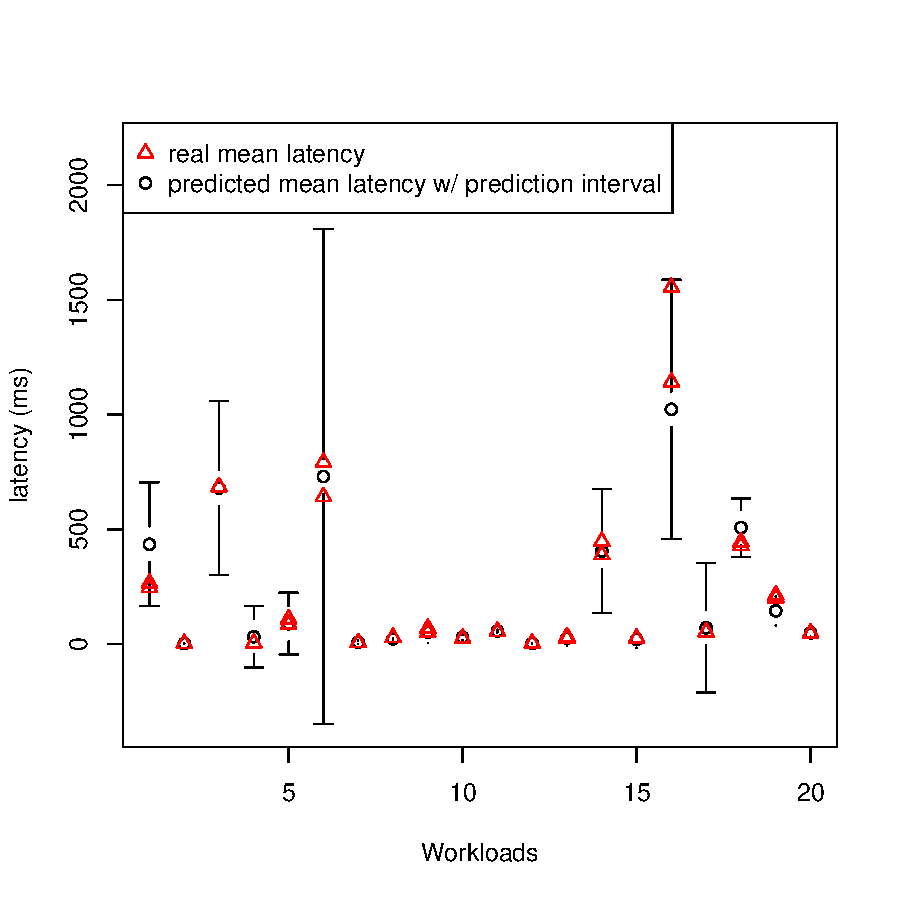
\includegraphics[width=0.6\columnwidth, clip, trim=0 0.2in 0 0.7in]{figure/prediction_interval2.pdf}
%\captionsetup{format=myformat}
\caption{The average latency (over 20 second intervals) observed from
  20 different workloads (running on separate virtual disks) on 4
  different test data stores during 1 hour interval.  The max and min
  latency is plotted. Also plotted are the model's 95\% prediction
  intervals.}
\label{predInterval}
\end{figure}

Perhaps the most significant benefit of our model is its ability to provide a prediction interval at pre-defined confidence for its predictions.
\figurename~\ref{predInterval} shows the average latencies of 20 different virtual disks running different workloads randomly selected from our test vector on four test data stores.
The average was evaluated over two minutes.
The predicted latency and its corresponding interval (shown as the error bar)  was calculated using our model at 95\% confidence (allowing 5\% of measurements to be outside of the prediction interval).

\figurename~\ref{predInterval} shows that the predictions can be off by up to $500\mathit{ms}$ (\emph{workload 16}).
However, all measurements fall within the prediction interval.
In fact, out of 1600 workloads ran against 4 data stores in the previous experiment, our model failed to capture the measured latency within its prediction interval 423 times which is 6.6\% (close to predefined 5\%) of 6400 predictions made.

Another interesting thing is that there were roughly 5\% of workloads whose confidence interval is so large, like the \emph{workload 6} in \figurename~\ref{predInterval}, that the prediction itself is meaningless.
Pesto~\cite{gulati:2011} claimed that these workloads had specific characteristics (such as purely sequential) and can be filtered out.
However, we found them to be more of random occurrences and difficult to predict in advance.
By default, the prediction is done every 8 hours to consider the possible moves in current VMware products~\cite{epping:2011}.
However, we force prediction every 2 minutes and observed prediction interval change after 5 hours.
In theory, the prediction interval should converge after about 2 hours (12 measurements), however we found the convergence to take a much longer time.
We suspect the reason to be fluctuation in the workload.
A detailed analysis and speeding up this convergence will be our future work.

In short, our model is capable of providing prediction interval at a specified confidence level.
The level of confidence can be lowered to trigger more aggressive load balancing with tighter prediction interval.
On the other hand a higher confidence interval will result in moves that are only triggered when predicted benefit is large enough to over come the larger prediction interval.

\section{Handling Heterogeneous Data Stores}

\begin{figure}[!t]
\centering
\subfloat[Measured Relative Latency]{\label{slm}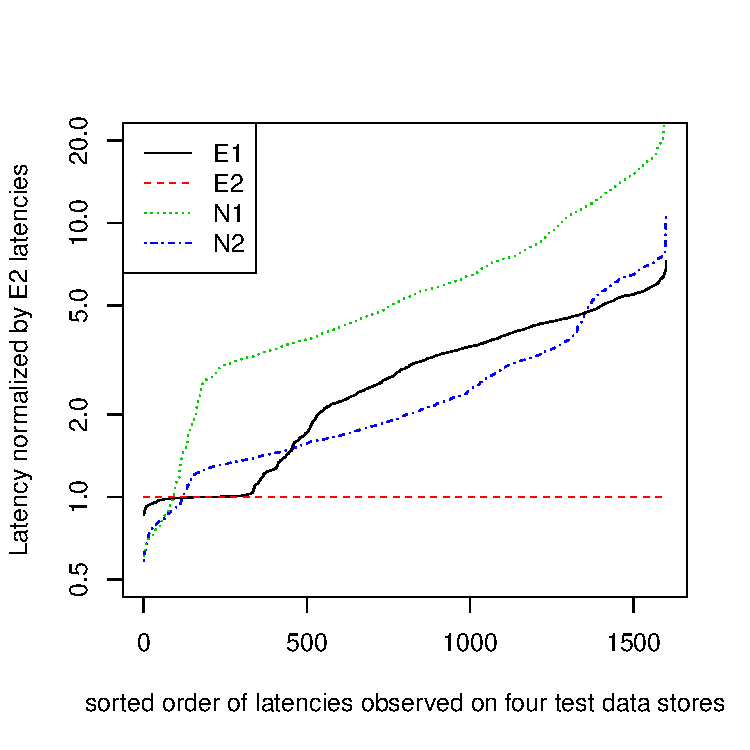
\includegraphics[width=0.33\textwidth]{figure/sorted_latency.pdf}}
\subfloat[Pesto Prediction - relative]{\label{slp}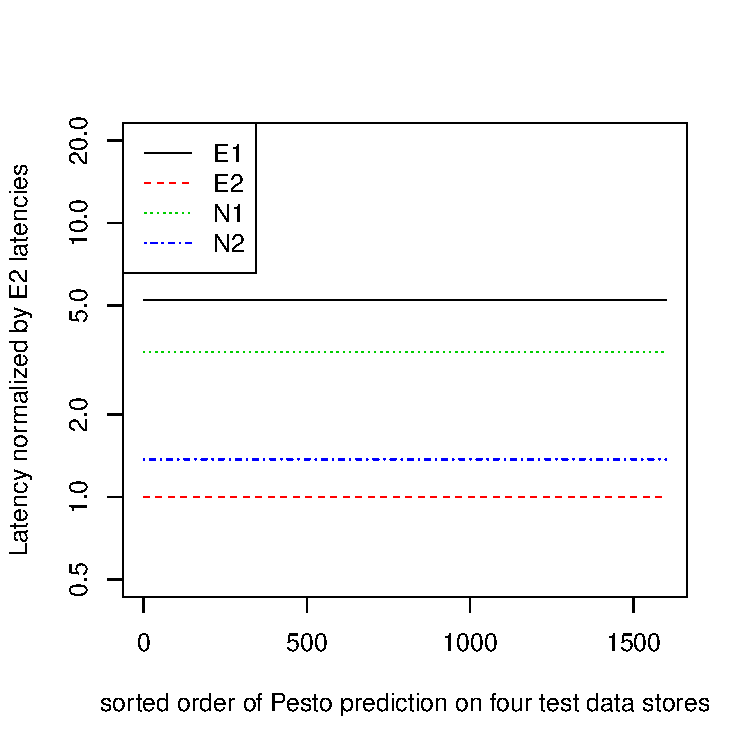
\includegraphics[width=0.33\textwidth]{figure/pesto_sorted_latency.pdf}}
\subfloat[Our Prediction - relative]{\label{slr}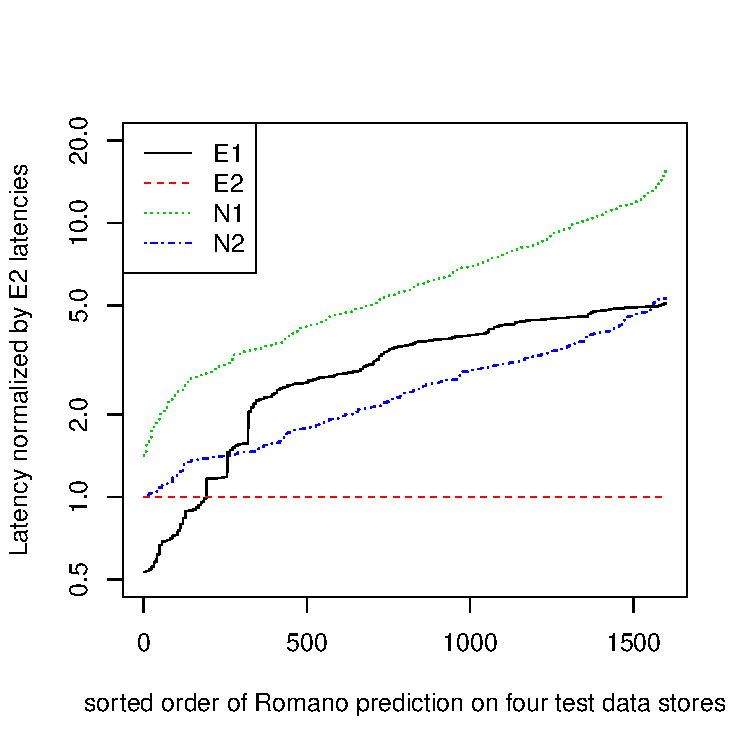
\includegraphics[width=0.33\textwidth]{figure/romano_sorted_latency.pdf}}
\caption{Sorted normalized latency plot for four test data stores.
It shows the relative latencies of E1, N1 and N2 compared to E2.
The 1600 latencies measured from each data store were normalized by E2 and than sorted.
The y-axis represents the normalized latency and the x-axis represents the sorted index.
The actual measurements as well as predictions from Pesto and our model are plotted.
%Pesto assumes a linear performance difference between the workloads so there is only a linear difference between the data stores regardless of the workloads.
%For the actual measurement, all four lines cross each other, suggesting that data stores are seldom slower than the other data store for all workloads.
%While Romano does not capture this effect fully, it does capture the most distinct features of real measurements.
}
\label{sortedLatency}
\end{figure}

In this section, we evaluate the models's ability to handle heterogeneous data stores using Pesto~\cite{gulati:2011} as the baseline.
Basil is not compared here since it only generates a single model across the data stores and can not handle heterogeneity.
Pesto injects a \emph{4KB, random and read-only} workload into the data store to derive the \emph{LQ-slope} for a given data store.
\tablename~\ref{pestolq} shows the Pesto LQ-slope of four test data stores.
Since each data store has a fixed LQ-slope regardless of the workload, running same workloads on multiple data stores will always result in constant ratio equal to the LQ-slope ratio.
\begin{table}[!t]
\centering
\begin{tabularx}{\textwidth}{
  >{\centering}X|
  >{\centering}X|
  >{\centering}X|
  >{\centering\arraybackslash}X
}
\hline
E1          &   E2      &   N1      &   N2 \\
\hline
25.798101   & 4.922433  & 16.666000 & 6.753044 \\
\hline
\end{tabularx}
\caption{Pesto LQ-slope of four test data stores.  The units are
  $\mathit{ms/io}$.  According to these slopes, E2 is the fastest data
  store and E1 is the slowest.}
\label{pestolq}
\end{table}
\figurename~\ref{slp} plots this effect.

\figurename~\ref{slm} shows the latency normalized by E2 latencies from running our \emph{test vector}.
As expected, most of latencies observed in other data stores are larger than that of E2 (with the smallest LQ-slope hence the fastest) but surprisingly, there exist some corner cases where even the slowest E1 out performs E2.
In fact, N1 seems to have the highest latency of all data stores on average even though its LQ-slope is lower than E1.
\figurename~\ref{slr} shows that our model is able to capture this relative difference fairly accurately.
For those corner cases where the model fails to capture the exact relative order of performance, the prediction intervals tend to be very large.
Therefore, Romano will not make any predictions for those cases with high confidence indicating that actions should not be made based on the prediction values only.

\begin{figure}[!t]
\centering
\subfloat[Pesto]{\label{rdPesto}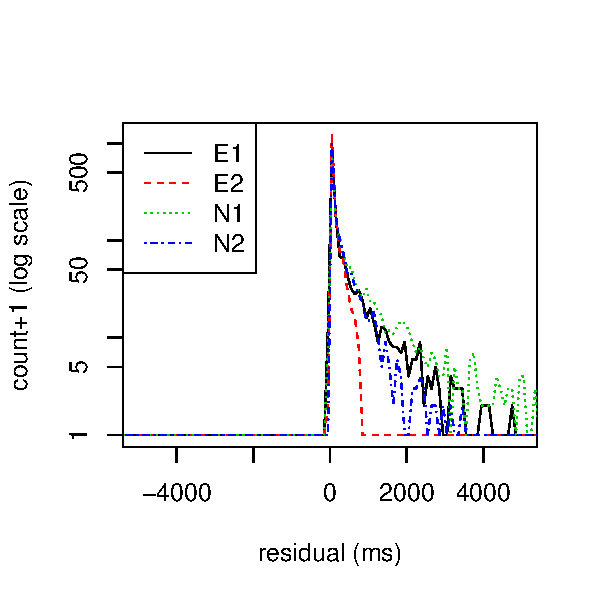
\includegraphics[width=0.5\textwidth]{figure/error_hist_compare_pesto.pdf}}
\subfloat[Proposed model]{\label{rdRomano}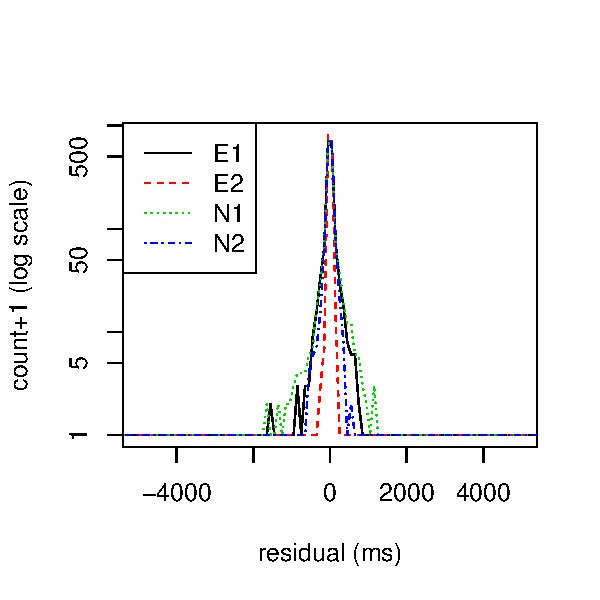
\includegraphics[width=0.5\textwidth]{figure/error_hist_compare_kromano.pdf}}
\caption{Distribution of residuals ($\epsilon$) for Pesto and Romano.
x-axis is the value of $\epsilon$ in $ms$.
y-axis is number of occurrences+1.
Addition of 1 was required to allow y-axis to be in log scale.
}
\label{residualDist}
\end{figure}
\figurename~\ref{rdPesto} shows that the residual ($\epsilon$) distribution of Pesto varies widely depending on the data store.
The accuracy of Pesto on a single data store provides little information about how it might do on another data store.
As the new data stores are introduced into the storage pool, the applicability of Pesto needs to be re-evaluated.

On the other hand, our model shows a much more even distribution across the data stores in \figurename~\ref{rdRomano}.
While there are some differences, prediction accuracy of our model is robust against the heterogeneity of data stores.
Furthermore, the model's prediction interval further improves its robustness by generating larger interval for the data stores that are difficult to model.
In short, proposed techinique provides robust and adaptive models across the heterogeneous data stores with a single framework.
%The justification was that except for the few extreme cases, \emph{``the variation of LQ-slope was limited to 15\%''}.

%assumes
%that the data stores only differ in terms of their capability to
%handle the outstanding IOs represented by latency increase per
%outstanding IO(\emph{LQ slope}). Romano assumes that each data store
%is affected by different components of workload characteristics in
%different ways as shown in \tablename~\ref{smodel}.

%\nohhyun{Figure 7:  The virtual disk labels should not be large random numbers.  Why not call them vdisk1, vdisk2,…?}

         % storage resource model
\chapter{Romano: IO Load Balancer}
\label{ROMANO}

%% Motivation
The cloud computing paradigm shift is built on virtualization.
Most IT organizations and cloud service providers have deployed virtualized data centers in an effort to consolidate workloads, streamline management, reduce costs and increase utilization.
Still, overall costs for {\em storage management} have remained stubbornly high.
Over its lifetime, managing storage is often four times more expensive than its initial procurement~\cite{merrill:2009}.
The annualized total cost of storage for virtualized systems is often three times more than server hardware and seven times more than networking-related assets~\cite{simpson:2010}.

A key enabler for virtualization adoption is ability for a virtual machine (VM) to be efficiently migrated across compute hosts at run time~\cite{clark:2005, wood:2007, nelson:2005}.
Consequently, VM live migration has been utilized to perform active performance management in commercial products for some time~\cite{vmware:2006}. 
Similarly, virtualization offers unprecedented dynamic control over storage resources, allowing both VMs and their associated virtual disks to be placed dynamically and migrated seamlessly around the physical infrastructure~\cite{mashtizadeh:2011}.

However, it is well-known that storage data associated with a VM is much harder to migrate compared to CPU and Memory state. 
Virtual disk migration time is typically a function of virtual disk size, size of the working set, source and destination storage state and capability, etc~\cite{mashtizadeh:2011}. 
Migration can take anywhere from tens of minutes to a few hours depending on those parameters.

Given the high expense of data migration, intelligent and automatic storage performance management has been a relevant but difficult research problem~\cite{gulati:2010, gulati:2011}. 
Virtualized environments can be extremely complex, with diverse and mixed workloads sharing a collection of heterogeneous storage devices. 
Such environments are also dynamic, as new devices, hardware upgrades, and other configuration changes are rolled out. 
Our goal of supporting heterogeneity is critical since data center operators want to keep the flexibility of buying the cheapest hardware available at any given time.

%% Problem
The key to automated management of storage lies in the ability to predict the performance of a workload on a given storage system.
Without it, an experienced user must determine manually if migrating a virtual disk is beneficial, a complicated task. 
Previous work~\cite{gulati:2010, gulati:2011} has relied on a heuristic model derived from empirical data.

When considering automated load balancing, the simplest approach would be to observe utilization of all data stores and offload a virtual disk from the most heavily loaded data store to the least heavily loaded data store.

There are several problems with this approach but the main problem is the unpredictability of the benefit of the moves. 
In fact, there exists no guarantee that the moves will even be beneficial. Storage systems do not react to different workloads in a homogeneous manner. 
A workload may stress one storage system significantly more than the other depending on the storage system configurations and optimizations.

The second problem is the workload interference.
When multiple workloads are placed into a single storage systems, their effect on the storage system is not simply additive. While some workloads can be placed onto a single storage system and work with minimum interference, some experience huge performance hits.

Romano prediction model takes into account this heterogeneous response of storage systems and the interference between workloads improving the prediction accuracy by over 80\%. Once these problems are recognized, it is obvious that the load balancing is no longer a bin packing problem as suggested by previous works~\cite{gulati:2010, gulati:2011, singh:2008}.
Therefore, we introduce a new load balancing algorithm based on simulated annealing~\cite{kirkpatrick:1983} that optimizes the overall performance in a stochastic manner.
We show that Romano is capable of reducing the performance variance by 82\% and reduce the maximum latency observed by 78\%.

Romano makes following contributions.
\begin{description}
\item[Accuracy] Romano residuals are reduced 80\% on average compared to previous techniques. 
Furthermore, the residual is unbiased and does not propagate with recursive predictions.
\item[Robustness] Romano is able to specify the prediction interval which satisfies a specified confidence level.
We show that the resulting prediction interval captures real performance with surprising accuracy.
\item[Flexibility] Different storage systems have different response characteristics to different workloads. 
Romano captures these differences by quantifying the effect of workload characteristics as well as the interactions of those characteristics on a given storage system.
\item[Optimization] Romano load-balancing algorithm avoids having system state stuck in a local optimum, instead identifying a global pseudo-optimal state through recursive prediction. 
At the same time, it also ensures that the most beneficial migrations are performed first to maximize the benefit.
\end{description}

We have prototyped \romano on VMware's ESXi and vCenter Server products. 
Minimal changes were made to the ESXi hypervisor to collect additional stats for vCenter where the core of \romano is implemented.

\section{Romano Design}

\begin{figure}[!t]
\centering
\begin{tikzpicture}[node distance = 2in, auto]
\node[clod,
  minimum height=1.1in,
  minimum width=3in
  ] (VDP) {Virtual Disk Pool};
\node[block,
  text width=13em,
  node distance=1.3in,
  below of=VDP,
  minimum height=1in,
  minimum width=5.5in
  ] (RM) {
  \begin{minipage}[t][0.8in]{6in}
    Resource Manager
  \end{minipage}
  };
\node[block,
  node distance=0.1in,
  below of=RM
  ] (LB) {Romano \\ Load \\ Balancer};
\node[block,
  right of=LB,
  node distance = 1.8in
  ] (RPM) {Romano \\ Performance \\ Model};
\node[block,
  left of=LB,
  node distance = 1.8in
  ] (RIM) {Romano \\ Aggregation \\ Model};
\node[clod,
  node distance=1.3in,
  minimum height=1.1in,
  minimum width=3in,
  below of=RM
  ] (DSP) {Data Store Pool};
\path[line] (VDP) -- (RM);
\path[line] (RM) -- (DSP);
\end{tikzpicture}

\caption{High level view of Romano.
Romano maps virtual disks onto pool of data stores to satisfy the load balancing policy.
}
\label{ov}
\end{figure}

Romano is a generic framework that allows automated load balancing of the virtual disks in a heterogeneous storage environment. 
Specifically, Romano predicts the storage performance using statistical techniques allowing the systems to relocate the virtual disks without the human
intervention.

\figurename~\ref{ov} shows an overview of Romano framework.
Romano sits within the Resource Manager which maps physical storage resources to the virtual disks.
Romano framework consists of \emph{Romano Performance Model}, \emph{Romano Aggregation Model} and a \emph{Romano Load Balancer}.
Romano Performance Model was described in Chapter~\ref{SPM}.
Romano Aggregation Model predicts the characteristics of multiple independent workloads when they are aggregated on a single data store.
Romano Load Balancer balances the workloads across heterogeneous data stores such that the mean and maximum latency observed by the virtual disks are minimized.

These components will be described in detail next.

\section{Romano Aggregation Model}
Predicting the performance of a data store given a workload is not always enough.
If the data store is already running different workloads, we need to figure out what the characteristics of aggregated workload will be.

In Basil, this is done by simply adding their workload parameter $\omega$~\cite{gulati:2011}.
This made sense under their assumption that all data stores react to different workloads in a similar manner.
Since $\omega$ represents the amount of work a data store has to process, aggregating workloads only involve addition of $\omega$'s.

Romano's workload model is a tuple of different combinations of characteristics.
It makes more sense to aggregate each characteristic separately.
In our closed loop assumption, aggregation of workloads does not affect the number of IOs each workload keeps in the system.
Therefore we can safely assume that the \emph{Outstanding IO}s~($\OIO$) will simply be added.

However, \emph{Size}~($\SIZE$) and \emph{Read Ratio}~($\READ$) can not be simply added together.
It needs to be averaged based on ratio of number of requests seen by the two workloads that are being aggregated.
Pesto weights each value by their $\OIO$, assuming that higher $\OIO$ means higher rate of requests.
However, $\OIO$ can be highly independent of arrival rate.
For example, imagine a process that generates 5 IO requests and issues additional IO whenever a request completes.
The arrival rate will only depend on the service rate of the requests and not on outstanding IOs which would be fixed at 5.
For Romano this weight to be used for averaging is already available as the inverse of \emph{LQ-slope}, which represents the throughput~($T$) from our performance model in Equation \ref{rpmf:eq}.

The \emph{Random}~($\RAND$) is tricky because the randomness of access cannot be defined per IO request and cannot be simply averaged.

\begin{figure}[!t]
\centering
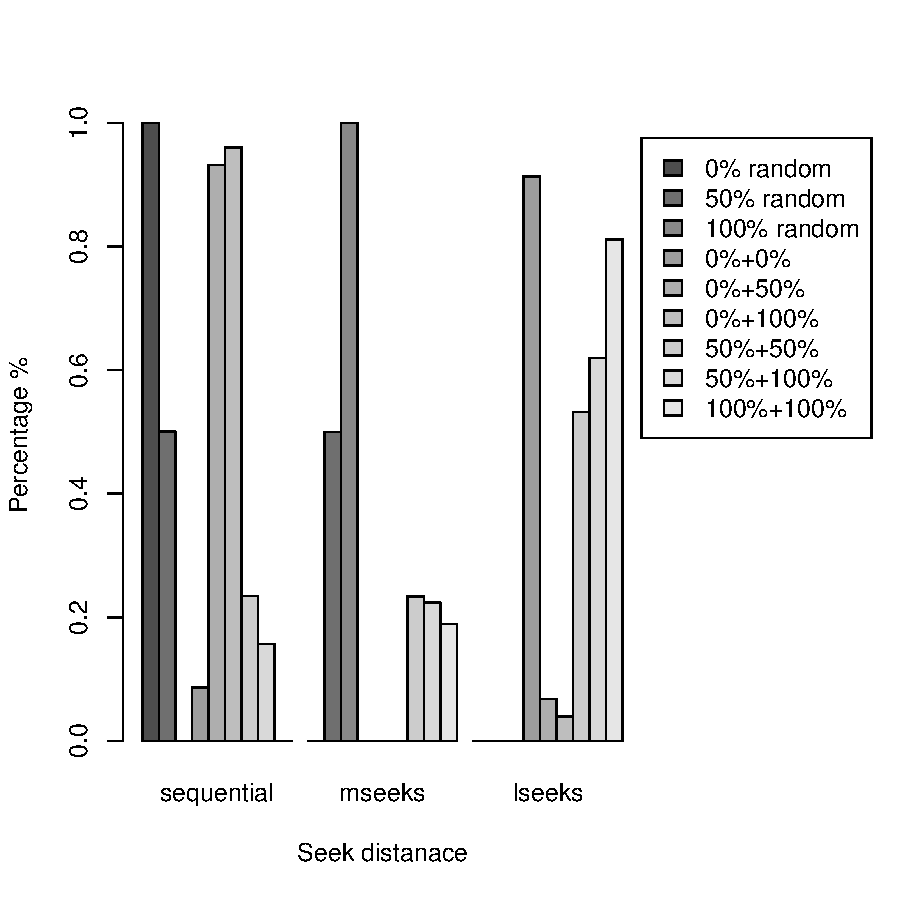
\includegraphics[width=0.7\textwidth]{figure/seek_profile.pdf}
\caption{Seek profile of different workloads.
Each color represents different mix of $\RAND$ for workload with $\SIZE=4\mathit{KB}$, $\READ=100\%$ read, $\OIO=1$.
\emph{mseeks} represents seeks done within a virtual disk and \emph{lseeks} represents seeks done across the virtual disks.}
\label{seekpr}
\end{figure}
\figurename~\ref{seekpr} shows the changes in the seek profile as you mix 0\%, 50\% and 100\% random workloads on E1 data store.
Our measurements show that the \emph{LQ-slope} for these workloads are 0.476, 17.6 and 35.8 respectively.
Therefore, the throughput~($T$), of these workloads are 2100.52, 56.77 and 27.93 respectively.

Note that \emph{mseeks} represents seeks within a virtual disk while \emph{lseeks} represents seeks across the virtual disks.
If we define the \emph{randomness} of the workloads as percentage of the seeks, the effect of aggregation is completely non-linear and hard to predict.
However, we make the following observations.
\begin{enumerate}
\item Mixing sequential workload and non-sequential workloads results in very low \emph{mseeks}.
\item The number of lseeks is determined by the lower throughput of two workloads.
\item The number of lseeks reduces the sequential and mseeks by the ratio of their average $T$.
\end{enumerate}
More formally,
\begin{align}
\overline{seq}&=\frac{\mathit{seq}_1T_1*\mathit{seq}_2T_2}{T_1+T_2}\label{r1}\\
\mathit{seq}&=\overline{seq}-(\overline{seq}*\mathit{\%lseek})\label{r2}\\
\mathit{\%lseek}&=\frac{\min(T_1,T_2)}{T_1+T_2}*2*\overline{seq}\label{r3}
\end{align}
which can be solved for ${\RAND}=1-\mathit{seq}$ to be:
\begin{equation}\label{randFun}
R_{\mathit{aggr}}=f_{\RAND}({\RAND}_1, {\RAND}_2, T_1, T_2)
=1-\frac{T_1T_2(1-{\RAND}_1)(1-{\RAND}_2)(1+2\min(T_1,T_2))}{T_1+T_2}.
\end{equation}
Equation \ref{r1} is a simple throughput weighted average of the $sequential\%$ representing average $mseeks$.
However, this does not account for additional seeks due to serving multiple virtual disks.
Therefore Equation \ref{r2} subtracts the amount of $lseeks$ from the $sequential\%$.
Note that the $\%lseek$ in the equation represents the percentage of $lseek$s.
Intuitively, the storage system is typically serving the high throughput workload and occasionally seeks to low throughput workload which causes the $lseek$.
Therefore, Equation \ref{r3} calculates the amount of $lseeks$ which is proportional to the ratio between the low throughput and the total throughput.
This value is multiplied by $2*\overline{seq}$ since almost every $lseek$ between the sequential workload is matched by a $lseek$ in the opposite direction to serve both virtual disks.

\begin{figure}[!t]
\centering
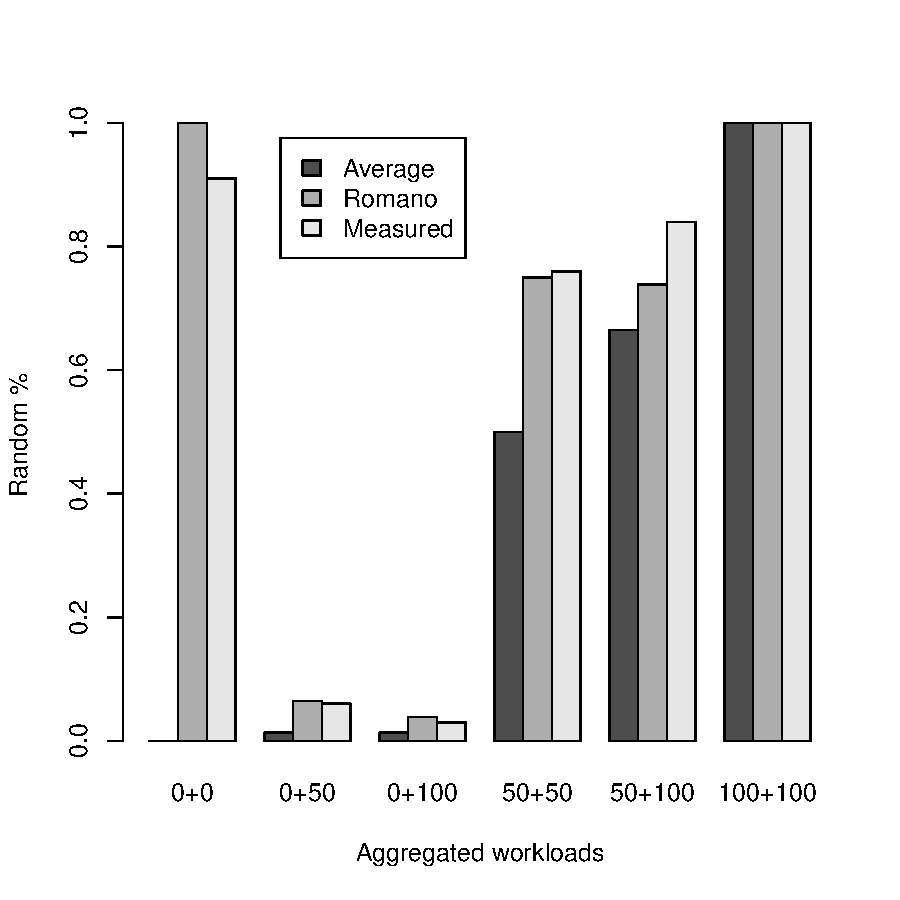
\includegraphics[width=0.7\textwidth]{figure/random_accuracy.pdf}
\caption{Comparison of $f_R$ and $T$ weighted average for the randomness of aggregated workloads.
Each color represents different methods.
Other characteristics are fixed at $S=4\mathit{KB}$, $\READ=100\%$ read, $\OIO=1$.
}
\label{randmix}
\end{figure}
\figurename~\ref{randmix} shows the result of $f_{\RAND}$ against simple $T$ weighted average.
The maximum and average error of doing $T$ weighted average is 100\% and 48\% respectively.
For $f_{\RAND}$ these values are 28\% and 5\% respectively.
The maximum error in both cases are when aggregating two completely sequential workloads whose resulting ${\RAND}_{\mathit{aggr}}$ has inherently high variance.

Putting it together, \emph{Romano Aggregation Model} is;
\begin{equation}\label{sumFun}
(\RAND_{\mathit{new}}, \READ_{\mathit{new}}, \SIZE_{\mathit{new}}, \OIO_{\mathit{new}}) \\
  = (f_{\RAND}({\RAND}_i, T_i), \frac{\sum_{i} {\READ}_i T_i}{\sum_{i} T_i}, \frac{\sum_{i} {\SIZE}_i T_i}{\sum_{i} T_i}, \sum_{i} {\OIO}_i)
\end{equation}
where aggregating more than 2 workloads require $f_{\RAND}$ to be recursively applied to the workloads.
In practice, this is naturally done since only a single virtual disk is migrated at a time.

\subsection{Romano Load Balancer}
The \emph{Romano Load Balancer} is different from traditional load balancers~\cite{gulati:2010, gulati:2011, singh:2008} in two ways.
Firstly, it optimizes the global state rather than a single storage migration.
Secondly, it is proactive.
The balancing mechanism does not wait until a overutilization is detected.
It continuously adjust the overall state whenever possible to ensure that systems are less likely to be over-utilized.
This is made possible by Romano's accurate and robust modeling techniques.

\paragraph{Merit Metric}
Our load balancing goal is to minimize the overall latency while reducing the maximum latency.
To represent both aspect of our goal with a single metric, we define Romano load balancing metric of Merit~($M$) to be the form;
\begin{equation}\label{merit}
M=\left(\sum_iP_i^\alpha\right)^\frac{1}{\alpha}
\end{equation}
where $\alpha$ controls the weight on the maximum latency.
For example, if $\alpha$ is 1, $M$ is simply the sum of all latencies.
However, as $\alpha$ becomes larger, more weight is given to high latencies.
Our experiment shows that 5 is a reasonable value for $\alpha$.
However, further exploration of $\alpha$ space is left for the future work.

\paragraph{Load Balancing}
\begin{algorithm}[!t]
\DontPrintSemicolon
\SetKw{updateMerit}{updateMerit}
\SetKw{minimizeMerit}{minimizeMerit}
\SetKw{loadBalance}{loadBalance}
\SetKwInOut{Input}{input}\SetKwInOut{Output}{output}
\updateMerit($W_{cand}, S_{cand}, \Phi$)
\Begin {
  $W_{src}\leftarrow getW(getS(W_{cand}, \Phi), \Phi)$\;
  $W_{dest}\leftarrow getW(S_{cand}, \Phi)$\;
  $W'_{src}\leftarrow$aggregate($W_{src}-W_{cand}$)\;
  $W'_{dest}\leftarrow$aggregate($W_{dest}+W_{cand}$)\;
  $P'_{src}\leftarrow$predict($S_{src}$, $W'_{src}$)\;
  $P'_{dest}\leftarrow$predict($S_{dest}$, $W'_{dest}$)\;
  \Return{merit($P'_{all}$)}
}
\minimizeMerit($\Phi_i, M_i$)
\Begin{
  $\Phi\leftarrow \Phi_i$;
  $M\leftarrow M_i$;
  $\Phi_f\leftarrow \Phi_i$;
  $M_f\leftarrow M_i$;
  $K\leftarrow 0$;
  \While{$K<K_{max}$} {
    $T\leftarrow$temperature($k/k_{max}$)\;
    $W_{cand}\leftarrow$randomChoose($W_{all}$)\;
    $S_{src}\leftarrow getS(W_{cand}, \Phi)$\;
    $S_{cand}\leftarrow$randomChoose($S_{all}-S_{src}$)\;
    $M'\leftarrow$updateMerit($W_{cand}, S_{cand}, \Phi$)\;
    \If{$G(M, M',T) >$ random()}
      {$\Phi\leftarrow$($W_{cand} \rightarrow S_{cand}$)\;
      $M\leftarrow M'$}
    \If{$M<M_f$}{
      $\Phi_f\leftarrow (W_{cand}\rightarrow S_{cand})$\;
      $M_f\leftarrow M'$\;}
    $K \leftarrow K+1$
  }
  \Return{$\Phi_f, M_f$}
}
\loadBalance($\Phi_i$)
\Begin{
  $M_i \leftarrow$merit($\Phi_i$);
  $\mathit{Mlist}\leftarrow \emptyset$\;
  $(\Phi_f, M_f) \leftarrow$minimizeMerit($\Phi_i, M_i$)\;
  \ForEach{$W \in \Phi_f$}{
    \If{$getS(W, \Phi_f) \ne getS(W, \Phi_i)$}{
      $\mathit{MoveCandidate} \leftarrow W$\;
    }
  }
  \While{MoveCandidate} {
    \ForEach{$W \in$ MoveCandidate}{
      $M' \leftarrow$ updateMerit($W, getS(W, \Phi_f), \Phi_i$)\;
      append($\mathit{Mlist}, (M',W,getS(W, \Phi_f))$)\;
    }
    sortDescendingByM($\mathit{Mlist}$)\;
    $(M, W, S) \leftarrow \mathit{Mlist}[0]$\;
    Move($W$, $S$)\;
    $M_i \leftarrow $ updateMerit($W, S, \Phi_i$)\;
    $\Phi_i \leftarrow (W \rightarrow S)$\;
    $\mathit{MoveCandidate} \leftarrow \mathit{MoveCandidate}-W$\;
  }
}
\caption{Romano Load Balancing Algorithm using Simulated Annealing}\label{algo}
\end{algorithm}
Romano uses \emph{simulated annealing}~\cite{kirkpatrick:1983} to optimize the overall placement and then makes moves that result in maximum reduction of $M$.
The reason for the first step is that greedy approaches used in previous works~\cite{gulati:2010, gulati:2011, singh:2008} could result in a local optimum that is far from the global optimum.
The solution cannot be greedy since any optimal sub-placement needs to be reevaluated once a new workload is added due to the aggregation function.
Adding a new data store is worse since every data store has its own performance model.
While the simulated annealing process does not necessarily result in optimal placements, it is guaranteed to be better than finding a local optimal if the algorithm can remember the best state it has seen so far~\cite{granville:1994}.

However, the resulting state may require too many workloads to be migrated.
Therefore, once the target state is defined through simulated annealing, we use a greedy method to get there.
This way, we can make moves that result in the largest reduction of $M$ while always moving towards the optimal state.
Of course, there may be a move that results in an even larger reduction but the move may prohibit the possibility of further reduction of $M$.

Algorithm \ref{algo} outlines the Romano load balancer.
In this algorithm, $\Phi$ represents the current mapping of workloads to data stores.
$getS(W, \Phi)$ represents the data store on which $W$ is mapped in current State $\Phi$ while $getW(S, \Phi)$ represents all the workloads mapped onto data store $S$ in state $\Phi$.
\emph{updateMerit} function takes the current system state~(all Workload mappings and their performance) and calculates new \emph{Merit} value.
Note that our goal is to minimize the Merit value.
The \emph{aggregate} function is \emph{Romano Aggregation Model} and \emph{predict} function is \emph{Romano Performance Model}.
Therefore, \emph{updateMerit} function is given a workload candidate to be migrated and destination data store.
New aggregated workloads are calculated and their performances are predicted.
Given the new performances of source and destination data stores, global merit is recalculated.
The \emph{minimizeMerit} function uses simulated annealing to minimize the Merit value.
The \emph{temperature} function and $G$ functions are taken from the earlier works on simulated annealing~\cite{kirkpatrick:1983}.
The \emph{temperature} function simply divides $k/k_{max}$ by $1.2$ every iteration.
$G$ function returns 1 if current merit is lower than previous merit so that the move is always accepted, but returns $e^{(M-M')/T}$ when current merit value is higher.
Therefore, there exists a finite chance of accepting a move even when the merit increases.
This probability decreases fast with the number of iterations and the difference between the new and old merit values.
With every iteration, the function chooses a random workload to move and a random destination data store.
New merit is calculated and the move is either rejected or accepted based on the value returned by $G$ and a random number between 0 and 1.
All our experiments required less than 200 iterations to complete.
The convergence rate of simulated annealing is difficult to predict without any structural information of the state space.
However, since we do not need the absolute minimum $M$, we can simply fix the maximum number of iterations to a reasonable number and choose the best state found.
The \emph{loadBalance} function takes the current state~($\Phi$) and calls on \emph{minimizeMerit} function to determine the pseudo-optimal mapping of $W$ on $S$.
Once the mapping is determined, it uses a greedy approach to determine which moves to execute. \emph{updateMerit} function is called on all possible moves to determine the next move.
Note that \emph{updateMerit} function executes in $O(1)$.
The process is repeated until the pseudo-optimal mapping is reached.

In practice, it is unlikely that all the moves will be carried out due to the cost involved with the migration. Furthermore, the workload themselves are going to change over time.
Therefore, Algorithm \ref{algo} will periodically rerun \emph{minimizeMerit} function and continually transition the system towards the newly found pseudo-optimal state without ever actually getting there.

\subsection{Workload Aggregation}

%\nohhyun{5.3  I don’t understand equations 23-25.  What do these parameters mean for a workload?  I tried to compare them to previous equations but could not find a matching format.  I can kind of figure out that C is more random than the others, B is read only, C has small IO size, but I don’t understand the OIO field. }
%Our experiment takes two three workloads to be ran on a single data store:
To test the effect of workload aggregation, we need to able to generate a repeatable workload.
\begin{table}
\centering
\begin{tabularx}{\textwidth}{
  X|
  >{\centering}X|
  >{\centering}X|
  >{\centering\arraybackslash}X
}
\hline
Workload      & $\mathit{IOSize}$ & $\mathit{Read\%}$ & $\mathit{Random\%}$ \\
\hline
Web File Server & 4KB             & 95\%              & 75\% \\
Web File Server & 8KB             & 95\%              & 75\% \\
Web File Server & 64KB            & 95\%              & 75\% \\
Support DB & 1MB         & 100\%             & 100\% \\
Media Streaming & 64KB            & 98\%              & 0\% \\
SQL Server Log  & 64KB            & 0\%               & 0\% \\
Web Server Log  & 8KB             & 0\%               & 100\% \\
OLTP DB         & 8KB             & 70\%              & 100\% \\
Exchange Server & 4KB             & 67\%              & 100\% \\
Workstation     & 8KB             & 80\%              & 80\% \\
VOD             & 512KB           & 100\%             & 100\% \\
\hline
\end{tabularx}
%\captionsetup{format=myformat}
\caption{Workload characteristics suggested by Wang~\cite{wang:2009}.
These workloads are used to ensure repeatable experiments.
%\cite{workload-suggestion}
}
\label{test_wl}
\end{table}
We use the workload settings shown in \tablename~\ref{test_wl} to simulate the real workloads.
Previous works have shown that synthetic workloads do a good job of representing real workload's performance characteristics when the parameters are extracted from the real workloads~\cite{tarasov:2012, park:2011}.

All possible combinations of two workloads were chosen from the 11 workloads shown in \tablename~\ref{test_wl} resulting in 55 combinations.
In Romano workload characteristics space, aggregating 2 workloads and 3 workloads are the same since the aggregation process is commutative and associative.
$\OIO$ was randomly assigned from 1 to 3. The test was repeated on two data stores for which the Romano model performed worst (see \figurename~\ref{rdRomano}).

The workload aggregation method used in Pesto~\cite{gulati:2011} is to average their workload metric $\omega$ weighted by $OIO$.
To isolate the effect of workload aggregation, we average individual workload characteristics weighted by $\OIO$ and use \emph{Romano Performance Model} to predict the latency.
\begin{figure}[!t]
\centering
\subfloat[Sample of latency prediction]{\label{aggrPred}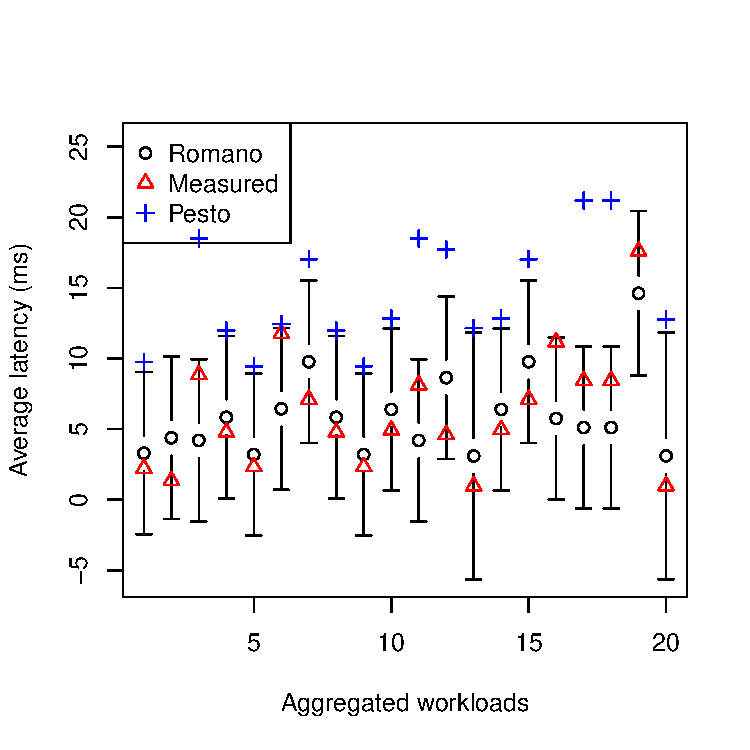
\includegraphics[width=0.625\textwidth]{figure/aggr_result.pdf}}
\subfloat[Residuals box plot]{\label{aggrRes}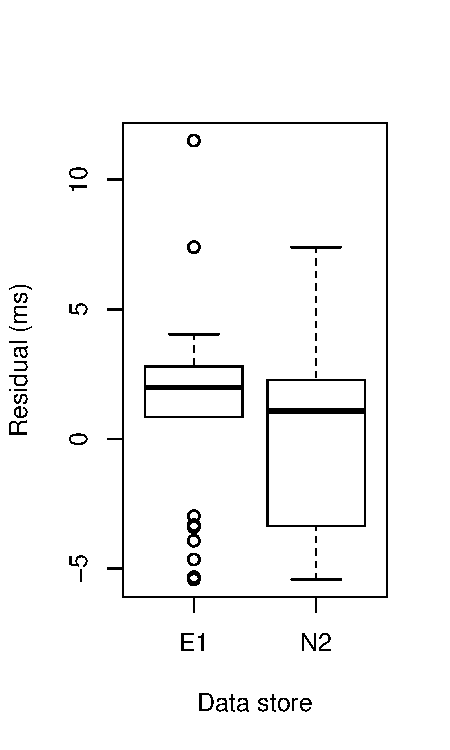
\includegraphics[width=0.375\textwidth]{figure/aggr_error.pdf}}
%\captionsetup{format=myformat}
\caption{Result of workload aggregation.
Two Workloads from \tablename~\ref{test_wl} were placed randomly across two data stores, E1 and N2.
\figurename~\ref{aggrPred} shows 20 randomly sampled results from 110 placements on both data stores (55 each).
\figurename~\ref{aggrRes} shows the residual of all 55 placements on E1 and N2.
}
\label{aggr}
\end{figure}

The result is shown in \figurename~\ref{aggr}.
\figurename~\ref{aggrPred} shows the latency from 20 randomly selected experiments as well as the prediction interval of Romano.
Only in 1 case, Romano failed to capture the latency within its prediction interval.
In fact, only 3 out of 110 cases (2.7\%) showed Romano failing to capture the measure latency.
This is better performance than specified 5\% confidence level.
We believe that this is due to the unbiased nature of Romano residual shown in \figurename~\ref{rdRomano}.
As the workloads are aggregated, the residuals ($\epsilon$) of \emph{LQ-slope} prediction, used for workload aggregation, are more likely to cancel each other out.

The accuracy of Pesto's approach of $\OIO$ weighted average does not seem too bad at first but there are some cases where the prediction won't even register on the \figurename~\ref{aggrPred} (workload 2 and 16).
This is especially true if the workloads running together are highly skewed such that one workload has much higher throughput than the other.
This verifies our assumption that the workload should be aggregated based on its throughput rather than $\OIO$.
his is especially true if the workloads running together are highly skewed such that one workload has much higher throughput than the other.
This verifies our assumption that the workload should be aggregated based on its throughput rather than $\OIO$.
\figurename~\ref{aggrPred} also shows that while Pesto consistently overpredicts the aggregated latency, Romano residuals are more unbiased shown in \figurename~\ref{aggrRes}.

Another interesting result was that all 3 cases where Romano failed were observed on E1 data store.
This is as expected from the amount of outliers shown in \figurename~\ref{aggrRes}.
We believe that amount of uncertainty introduced by workload aggregation is different on each data store.
We leave the further investigation to future work.

\subsection{Load Balancing Using Romano}
%\nohhyun{Section 5.4, the actual algorithm for load balancing is not clear. The pseudo-code given is clearly wrong and it isn't obvious what is actually meant.  In particular, I can't tell how you balance between placing a virtual disk on the data store that is best suited for it, against the other virtual disks that are also best suited to that data store.}
\begin{figure}[!t]
\centering
\subfloat[Initial data stores latencies.]{\label{lb_init}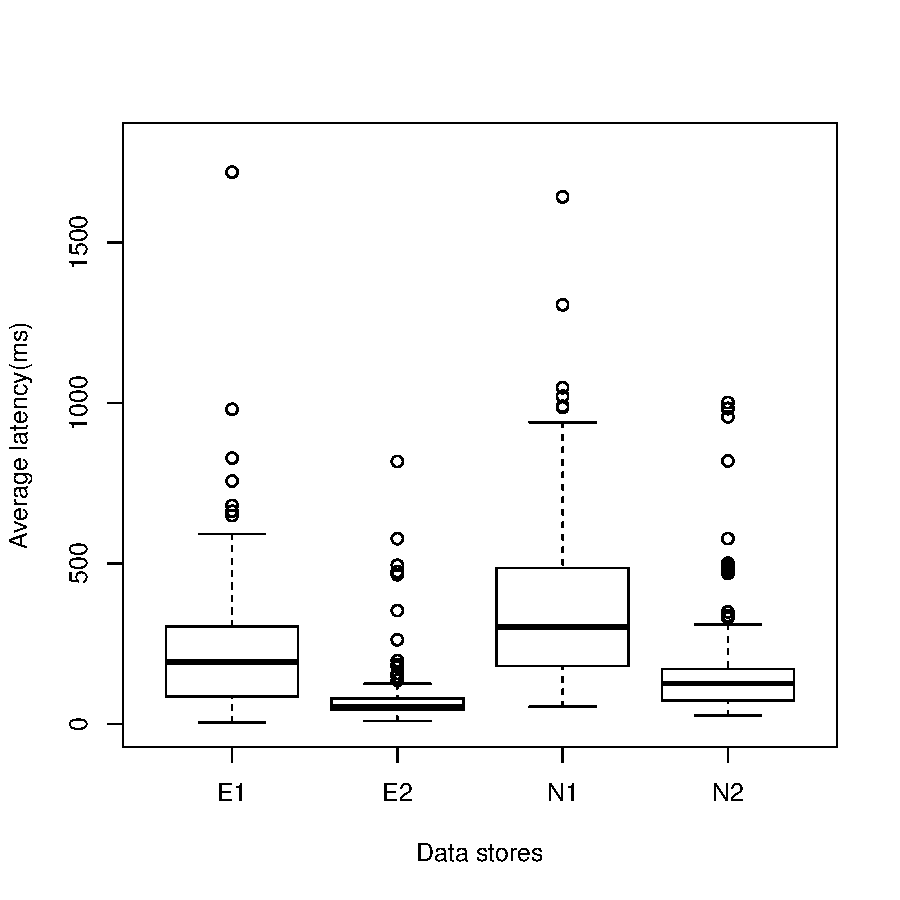
\includegraphics[width=0.3\textwidth]{figure/initial_datastore_latency.pdf}}
\subfloat[Result of Basil load balancing]{\label{lb_basil}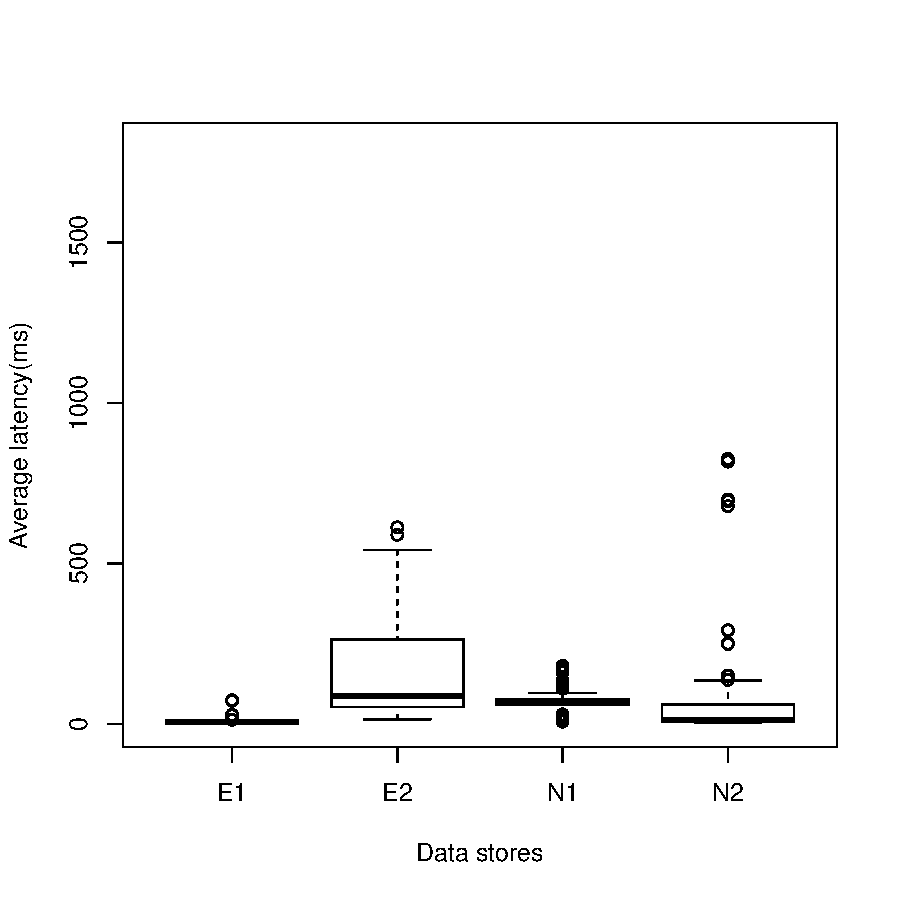
\includegraphics[width=0.3\textwidth]{figure/basil_datastore_latency.pdf}}
\subfloat[Result of Romano load balancing.]{\label{lb_after}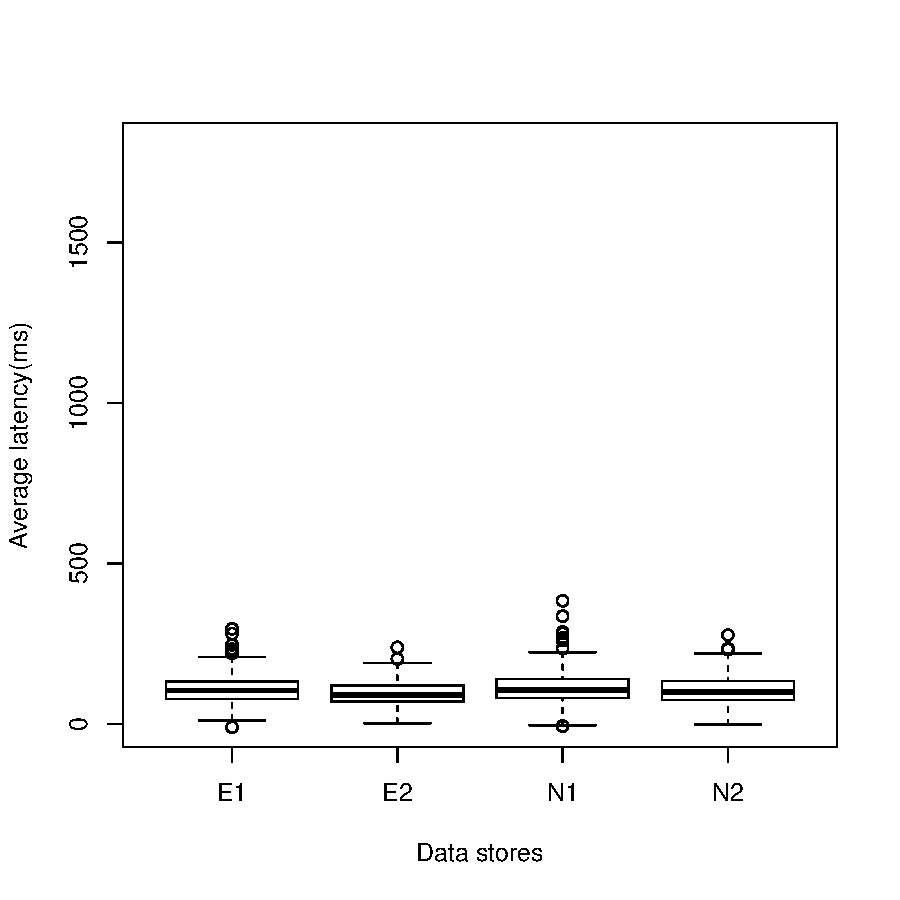
\includegraphics[width=.3\textwidth]{figure/romano_datastore_latency.pdf}}
\caption{Boxplot of average data store latencies on 50 different test cases.
Each test randomly placed 8-14 workloads from \tablename~\ref{test_wl} (allowing repetition) on 4 data stores.
Basil's greedy approach is compared with Romano's random optimization technique.
}
\label{load_bal}
\end{figure}

In this section we randomly placed 8-14 workloads from \tablename~\ref{test_wl} allowing repetition on 4 data stores.
Romano load balancing algorithm from Algorithm 1 was ran to optimize the data placement by moving a single virtual disk at a time.
The experiment was repeated 50 times.

\figurename~\ref{load_bal} shows the aggregated result of load balancing using Basil and Romano.
It should be noted that the load balancing algorithm deployed by Basil and Pesto are the same.
Both Basil and Romano does a good job of reducing the average latency by 47\% and 52\% respectively.
However, the variance is reduced by 82\% by Romano while Pesto reduces it by 37\%.
Most importantly, the maximum latency observed was reduced by 78\% with Romano while only 21\% by Pesto.

There are two factors which result in improved performance by Romano.
The first is the more accurate modeling.
Both Pesto and Basil assume that there exists only a constant performance difference between different data stores for any given workload.
Therefore, it has tendency to move virtual disks to a data store that is more powerful regardless of the workload.
Furthermore, their aggregation model is based on the outstanding IOs only.
This allows workload that do not performance well together to be placed on a single data store.
The result of these inaccuracies in the model forces the load balancing algorithm to place more workloads on the powerful data stores.
In fact 51\% of all the moves by Pesto were made to E2 data store compared to 28\% for Romano.
\figurename~\ref{lb_basil} shows that resulting E1 and N1 latencies are smaller than that of Romano while E2 and N2 exhibit large latencies that we would like to avoid.
In fact, Basil does not place any workload on E1 90\% of the time even though E1 actually has lower latency for most workloads than N1 as shown in \figurename~\ref{slm}.

The second factor is the load balancing algorithm itself.
Basil and Pesto uses a greedy approach~\cite{gulati:2010} which terminates the algorithm once no beneficial moves are found.
Romano uses simulated annealing to find the pseudo optimal placement first and than uses greedy approach to get to the optimal placement.
This allows Romano to avoid moves that may result in maximum benefit but prohibits any further moves that may provide additional benefits.

\begin{figure}[!t]
\centering
\subfloat[Basil]{\label{basil_mv}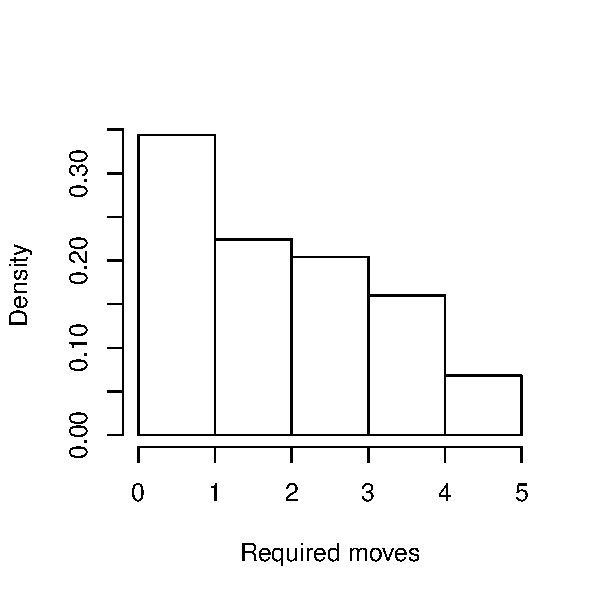
\includegraphics[width=0.5\textwidth]{figure/basil_required_moves.pdf}}
\subfloat[Romano]{\label{romano_mv}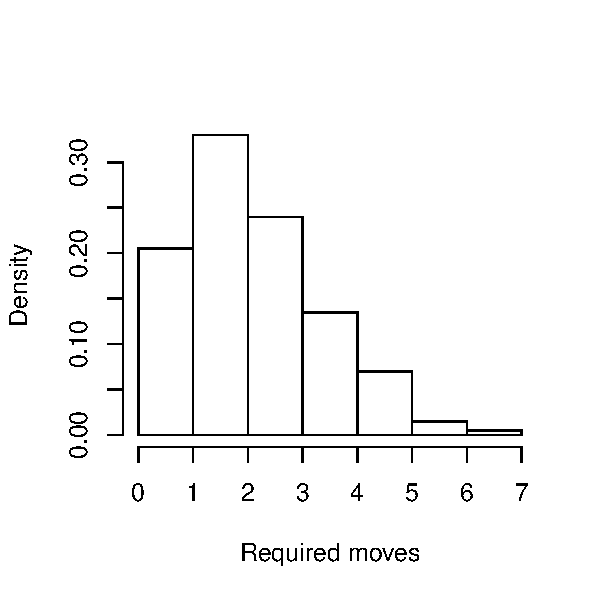
\includegraphics[width=0.5\textwidth]{figure/romano_required_moves.pdf}}
\caption{
The distribution of number of moves resulting from Basil and Romano.
}
\label{moves}
\end{figure}
\begin{figure}[!t]
\centering
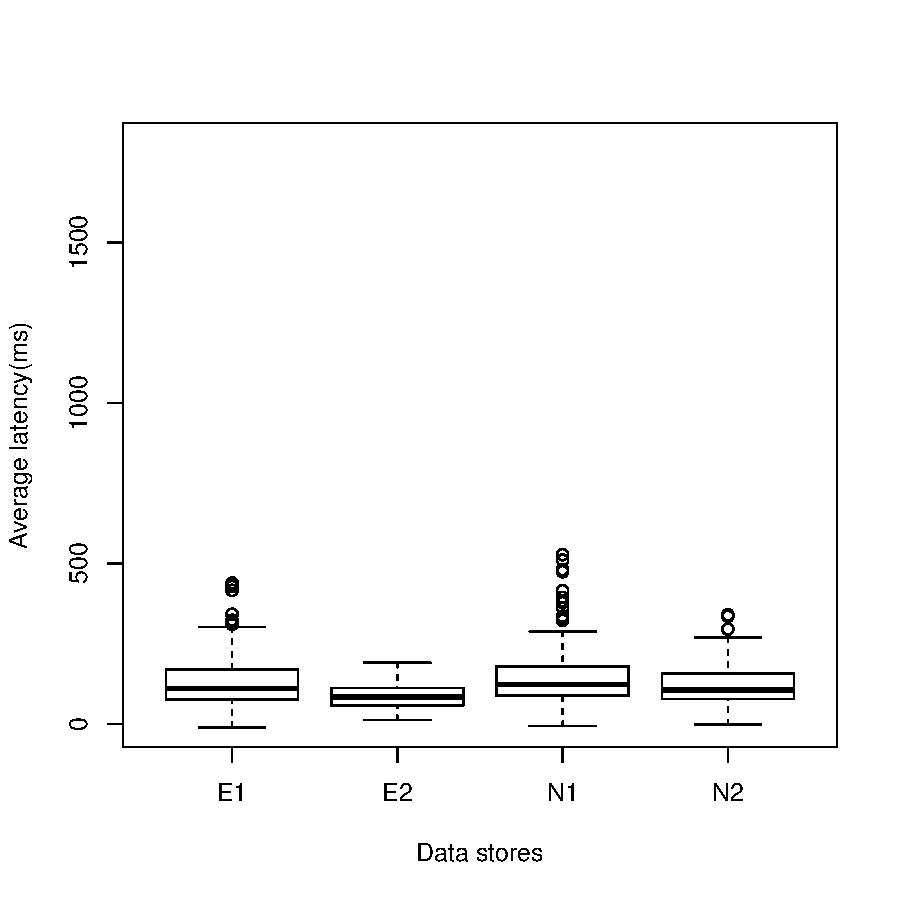
\includegraphics[width=\textwidth]{figure/romano_latency_2moves.pdf}
\caption{Data store latencies after maximum of 2 moves with Romano.}
\label{two}
\end{figure}
One limitation of this approach is that it does require more moves to be made.
\figurename~\ref{moves} shows the number of moves required for Basil and Romano.
On average Basil requires $2.2$ moves where as Romano required $2.6$.
Storage migration is expensive and should avoided if possible.
However, we show that even if we limit the maximum number of moves to 2, Romano still out performs Basil as shown in \figurename~\ref{two}.
This is due to the greedy approach in which Romano chooses moves once the pseudo-optimal placement is identified.
\begin{figure}[!t]
\centering
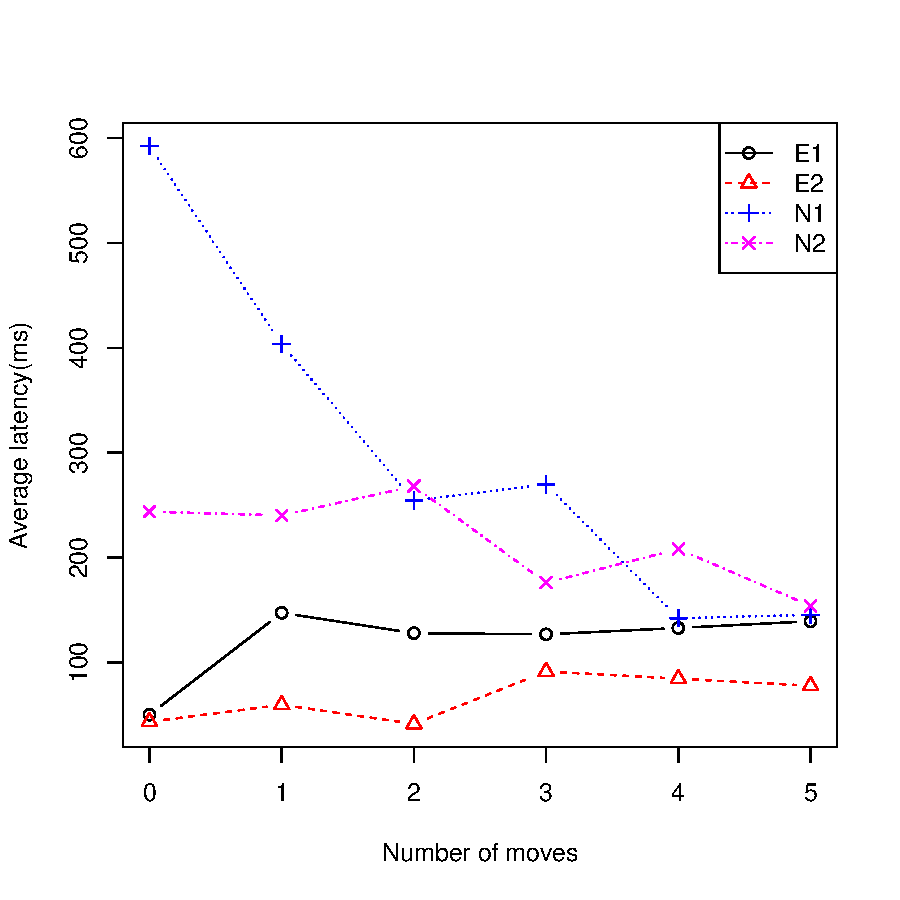
\includegraphics[width=\textwidth]{figure/23latency_reduction.pdf}
\caption{Typical Romano load balancing process with large number of moves.}
\label{proc}
\end{figure}
\figurename~\ref{proc} shows an example of latency changes for a single test case.
It is shown that most critical balancing is done within the first couple of moves.
%\nohhyun{5.4  About the pseudocode, why is D removed from the list when a virtual disk is assigned to it?  Can’t a data store handle more than one virtual disk depending on its performance characteristics?}
~
\section{Conclusion}\label{CONCL}
We have presented Romano, a load balancing framework for virtual disks
on heterogeneous storage systems. The kernel of Romano is a performance
predictor given a set of parameters that characterize the workloads and
the storage devices. We have shown that Romano can outperform
previous systems with same goals by up to 80\% in prediction
accuracy. This increased accuracy results in 78\% reduction in maximum
latency observed and 82\% reduction in variance while load balancing.

At a deeper level, Romano contributes a recognition that there is
inherent noise in storage system performance that is not easily dealt
with. Romano is capable of capturing this noise within the prediction
interval. As more data is gathered there is higher confidence that the
prediction interval will contain the measured latency.

Another key contribution of Romano is quantification of effect of
various workload characteristics and their interaction on heterogeneous
storage devices.
We have shown that the performance differences between data stores cannot be described with a single number. More specifically, we have shown that the storage performance must be described in terms of the workload.

The last contribution follows the second contribution. Since the performance of storage systems effectively change with the workload, the load balancing problem is no longer a bin-packing problem as previously believed.
Therefore we present a probabilistic approach to finding a pseudo-optimal mapping of workloads to the data stores.
It is important to mention that probabilistic approach is only used to find the final state of the system and the moves are actually made greedily to speed up the convergence and minimize the number of moves that has to be made.

We believe that Romano not only provides means for more efficient load
balancing but also in many other areas such as QoS management, power management and performance tunning in tiered storage.

Whereas Romano raises the bar on the accuracy of practical modeling
techniques, there remain ample opportunities for improvements in
future work. Better interference modeling between workloads when they
are placed on same data store is one such area where we are making
good progress. Another work in progress is to come up with a better
set of workload characteristics such that the workload description can
be more complete.
~
      % io load balancer
%%%%%%%%%%%%%%%%%%%%%%%%%%%%%%%%%%%%%%%%%%%%%%%%%%%%%%%%%%%%%%%%%%%%%%%%%%%%%%%%
% simulation.tex: Chapter on MC production:
%%%%%%%%%%%%%%%%%%%%%%%%%%%%%%%%%%%%%%%%%%%%%%%%%%%%%%%%%%%%%%%%%%%%%%%%%%%%%%%%
\chapter{Backup Workload and Data Deduplication}
\label{BW}
%%%%%%%%%%%%%%%%%%%%%%%%%%%%%%%%%%%%%%%%%%%%%%%%%%%%%%%%%%%%%%%%%%%%%%%%%%%%%%%%

Data deduplication provides a means to efficiently remove redundancies from large datasets. 
This process is made possible by first dividing up the data into segments and representing each segment with a much smaller hash value. 
A redundant segment of data is then easily identified through a hash table lookup. 
The efficiency of the process comes at the cost of possible data loss through hash collisions, thoug it is understood that the collision probability is negligible compared to the soft error rate of the storage system if an appropriate hash function is used~\cite{aronovich:2009, zhu:2008, bobbarjung:2006, muthitacharoen:2001}. 
Another performance factor is the granularity of compression which is limited to the size of duplicate segments. 
Two segments that are off by a single bit will result in no compression.  
	
%%Problem 
Despite these costs, data deduplication has steadily gained its place in backup~\cite{meister:2009, lillibridge:2009, zhu:2008}, archive~\cite{you:2005} and virtual machine storage solutions~\cite{smith:2008, jin:2009, clements:2009} due to its potentially huge reduction in storage space and IO elimination. 
However, as more and more systems opt to take advantage of data deduplication techniques, the variability in performance is becoming an issue. 
The cause of this variation can be catagorized into two factors, \emph{systemic variation} and \emph{input variation}. Systemic variation is caused by the use of different algorithms and techniques as well as the underlying hardware deployed in the deduplication systems. The input variation is caused by different characteristics of the input datasets. The systemic variation is critical from the deduplication system designers' and vendors' perspectives since it allows them to compare two systems directly. However, the input variation is typically more critical from the custumer's perspective when evaluating the potential benefits of data deduplication for different types of datasets.  

Current metrics for characterizing the datasets for data deduplication are overly simplified and often inaccurate. For example, the compression ratio ($\mathit{CR}$) is typically estimated using the \emph{average data change rate} ($\overline{\mathit{dcr}}$), which is the percentage of data change. Let $R$ be the required retention period. Assuming a full backup per unit time, the compression ratio is simply: 
\begin{equation}\label{dcr_est}
\mathit{CR}= \frac{\mathrm{Compressed\ Size}}{\mathrm{Uncompressed\ Size}}=\frac{1+(R-1)\cdot \overline{\mathit{dcr}}}{R}. 
\end{equation}
This model provides a simple estimation of the ompression ratio but it can also be very inaccuarate. We observed over 35\% error using the $\overline{\mathit{dcr}}$ to charaterize one of our datasets. One of our main contributions is providing a new set of metrics and models that allow much more accurate compression performance predictions to be made. In five out of six cases we test, the error reduction was over 50\% when compared with the $\overline{\mathit{dcr}}$ method.  

The main performance metrics for data deduplication systems are the compression ratio and the read/write throughput. While the latency could also be an issue for virtual machines, it can be mostly masked by high level caching and prefetching mechanisms. Unless specified otherwise, we use the term \emph{performance} to represent both the throughput and compression together. 

The throughput of the system is heavily dependent on both system and input factors. Thus, it is difficult to determine if one dataset outperforms the other in terms of throughput. However, there are features of datasets that are likely to benefit throughput in most systems. One obvious one is the compression ratio itself. A highly compressable dataset has lower IO requirements which in turn improves the throughput in most systems. The compression ratio is the most influential factor in determining the throughput. However, there are also other factors, such as spatial locality of the data segments and bursty arrival rates, which we examine in this paper. 

%%Contribution
Our main contribution in this paper is to provide a framework to characterize the input dataset for data deduplication systems. We 1) show that different datasets behave with a unique pattern that is quantifiable. Furthermore, we 2) provide analysis on how this pattern affect the deduplication system performance. As part of the framework, we 3) provide classification of segment types and their relations. We further provide parameters to show how the \emph{composition} of these segment types change over time. 

%%Paper organization
Section \ref{sys} will describe the data deduplication more formally and define set of essential characteristics of data deduplication systems. In Section \ref{dss}, we describe the datasets and the main attributes for which we characterize of the data. Section \ref{result} describes our analysis and Section \ref{appp} propose various applications of those results. Section \ref{rel} lists related works, Section \ref{lim} lists our limitations and Section \ref{con} concludes the paper.

\section{System Components}\label{sys}

\begin{figure}[!t]
\centering
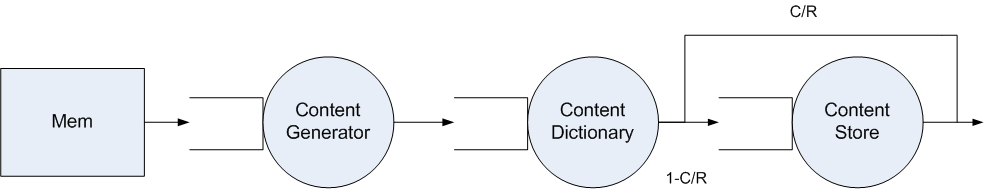
\includegraphics[width=3.5in]{figure/dedup/queue}
\caption{Our simplified deduplication system model. It is essentially 3 server open queuing system. At the content dictionary, C/R of the segments exit the system and 1-C/R of the segments are passed on to content store. All data are assumed to be immediately available at the memory and all three servers have exponentially distributed service time.} 
\label{queue}
\end{figure}

%dedup component
The deduplication process itself can be divided into largely three parts as shown in \figurename~\ref{queue}. First part of the process generates a sequence of segments from input data stream which we call the \emph{content generator}. In the second phase, the deduplication system generates a dictionary of segments which is in turn used to identify the duplicate segments which we call the \emph{content dictionary}. In the last phase, new segments are stored on a persistent storage system which we call the \emph{content store}. The later two components form a \emph{content addressable storage}(CAS).

%data component
The input data itself is another system component that affects the performance. To understand how the dataset affects the performance, it is described in terms of how the data components can be separated once it is deduplicated. The segments, regardless of how they are defined, are the smallest units of data in data deduplication. therefore, we define data as a sequence of segments rather than contiguous bits or characters. In this work, we show that the distribution of these different segment types completely describes how the dataset affect the deduplication performance.

\subsection{Content Generator}
The goal of the content generator is to maximize the redundant segments while minimizing the number of segments generated. 
These two goals often conflict with each other since the amount of duplicate data tends to increase with smaller segments size. 
This is due to the fact that the generation of segments are typically done in stateless manner to keep up with the huge data size and stringent throughput requirements. 
Recent papers try to overcome this limitation through a two level definition of contents~\cite{kruus:2010, bobbarjung:2006}. 
However, these approaches come at the extra computation cost and are applicable only when there are less stringent throughput requirements.

%segmentation types
These are the three most common methods to define the segment boundaries also known as the \emph{anchors}~\cite{zhu:2008, muthitacharoen:2001}.
\begin{itemize}
	\item \emph{File based}: A file boundary becomes the segment boundary.
	\item \emph{Size based}: The anchors are designated every $k$ bits which determines the boundaries for the segment. Therefore, any addition or deletion of data results in shifted anchors which is propagated until the end of the data stream. This effect is known as the \emph{boundary shifting problem}~\cite{muthitacharoen:2001}. 
	\item \emph{Content based}: An anchor is generated based on the content of the data which becomes the boundaries for the segments. Therefore the anchors are shifted together with the contents in the case of addition and deletion of the data. 
\end{itemize}

The \emph{content based} approach is the most popular method used in data deduplication due to the boundary shifting problem found in the size based method. 
Average, maximum and/or minimum segment size are usually specified for the content based approach. This allows system to expect segments of the bounded size which makes the segment handling simpler but also ensures that amount of size variation is limited which can cause loss of redundancy~\cite{eshghi:2005}.

%decoupling from the rest of the system
From the system perspective, the content generator is the source generator for the CAS. Typically, any information about the original data stream is lost after this point. This justifies our looking the dataset as a sequence of segments since beyond this point, the system is effectively decoupled from the original dataset. 

\subsection{Content Dictionary}
%hash
The content dictionary is typically a hash table which is keyed by hash of segments. Hash functions used typically provide one-way property as well as collision resistance. While only the collision resistance is required for correct functionality, one-way property is also attractive to ensure that the malicious users cannot corrupt the system by generating hash collisions.

For a large dataset, the content store itself becomes significantly large. 
To relax the memory requirements for the deduplication system, the content dictionary is typically stored on the disk~\cite{mandagere:2008, lillibridge:2009, zhu:2008, bhagwat:2009} . 
Only a portion is cached onto the memory at a time. Furthermore, any writes to the index table must be serialized which require expensive locks~\cite{clements:2009}. Therefore, the caching algorithm for the index table is one of the major performance factor within the deduplication system.

To avoid unnecessary accesses to the index table, Bloom filter~\cite{bloom:1970} is used to quickly determine segments that are not in the index table~\cite{zhu:2008}. While the backup stream typically exhibit an inherent spatial locality between the segment instances~\cite{zhu:2008}, more intelligent caching schemes that uses data similarities have also been proposed~\cite{lillibridge:2009, bhagwat:2009}.

Regardless of caching scheme, it is clear that content dictionary determines the data path for any given segment. While every segment must read the index table at least once, only the new segments result in it's update\footnote{This may not be strictly true if there exists a metadata information which must be updated within index table for duplicate segments as well. However, the fact that the new segments incur extra operations does not change.}. Furthermore, these new segments must be passed down to the content store to be store on the disk. Problem is more complicated for the read where segments maybe fragmented in various places both for the actual contents and the dictionary. A recent work duplicated heavily used segments over the physical disk such that the average seek time can be minimized~\cite{koller:2010}. However, such approach assumes small working set of segments and is heavily workload dependent.

In this work we assume nothing about the caching policy of the content dictionary or any other auxiliary data structure to minimize the access to the dictionary. We only assume that the different segment types results in different resource requirements in regular read/write operations. 

\subsection{Content Store}

Once the segments are identified as new content that needs to be stored, it is passed down to the content store to be processed. Various different mechanisms are possible. The content may already be on the disk and the content store only generates a logical mapping and freeing of segments~\cite{clements:2009, rhea:2008} or use log-based filesystem to optimize for the in-band writes~\cite{zhu:2008}.

The content store is not affected specifically by the deduplication system. While inherent \emph{copy-on-write} (COW) support of storage subsystem~\cite{bonwick:2003, dillon:2008} allows easier sharing of segments, the fundamental operations of underlying storage does not differ from dataset to dataset. Therefore, we focus mostly on the behaviors of the content dictionary in this paper. 

\subsection{Queuing Model}
The system can be viewed as simple open queuing system with three servers as seen in \figurename~\ref{queue}. We make very little assumptions of particular algorithms deployed. However, the functionality of each stage we have just described exists in all conventional deduplication systems. 
In this system, the arrival rate of segments at the \emph{content dictionary} is assumed to be exponentially distributed with the mean of average service rate at the \emph{content generator}. The probability of the arriving segments to be found in the dictionary is equal to the the compression ratio in which case it can by pass the \emph{content store}. If we assume that each outcome is independent, the arrival rate at content store is also exponentially distributed. However, we show that this is not true and is one of the factors that affect the throughput of the system.  

\subsection{Segment Classification}

\begin{figure}[!t]
\centering
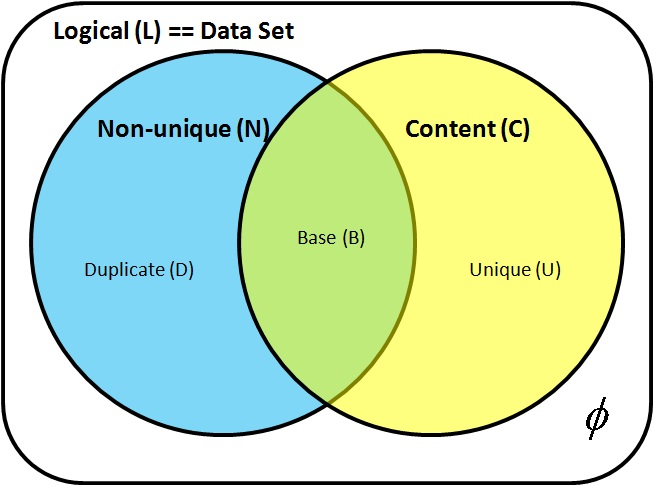
\includegraphics[width=3in]{figure/dedup/seg_classification.jpg}
\caption{Venn Diagram of Segment Sets. The \emph{logical segments} which is equivalent to the \emph{dataset}, can be grouped into two separate sets $N$ and $C$. The elements of $N$ are segments whose content occurs more than once in the dataset while the elements of $C$ are segments that must be stored in order to ensure no content information is lost from the dataset.}
\label{seg_class}
\end{figure}

We first define data segment as a tuple of \emph{offset} and \emph{size} within a dataset. Therefore every segment is uniquely identifiable regardless of its content. The only constraint under this definition is that the size of the data segment must be less than or equal to the size of the dataset. Also, the content of the data segment must exist within the dataset. There are no other restrictions to what may be defined as a segment. A dataset is then a mere concatenated sequence of data segments.

We begin classifying the data segments by defining the \emph{logical segments} which is the set of all segments from which you can reconstruct the original dataset through reordering only. Under this definition, a \emph{dataset} is nothing but an ordered list of logical segments. We also define \emph{unique segments} and \emph{non-unique segments}. The unique segments are a set of segments whose content is unique across the logical segments. Obviously the non-unique segments are the segments whose content is repetitive across the dataset. These non-unique segments have a unique property called the \emph{degree of repetition} which represents number of  times a particular content exist within a dataset.

From the perspective of the data deduplication system, the segments are really divided into segments whose contents must be stored and segments which can be represented only as a reference to an already stored segment. We further classify segments as either the \emph{content segments} or the \emph{duplicate segments} based on whether the content of the segment is required to reconstruct the logical segments. The content segments can be duplicated and reordered to construct the original dataset given the ordering information of contents. The duplicate segments are simply redundant contents whose only new information is the order of the content.

It is obvious from the two classifications that the duplicate segments must be the non-unique segments while the unique segments are content segments. This is shown in the \figurename~\ref{seg_class}. As shown in the figure, there exists an intersection of non-unique segments and the content segments that are called the \emph{base segments}. The base segments are minimum set of segments whose contents that must be stored to allow the deduplication system to reconstruct all the non-unique segments.

Therefore, the base segments, the unique segments and the duplicate segments are three sets of segments that are disjoint and whose union is the logical segments. A segment at any given time must be a member of one and only one of these sets.

We also define a relational parameter between these sets.
\begin{definition}[$\mathit{scr}$]\label{scr}
Segment compression ratio. $\mathit{scr} = \abs{C}/\abs{L}$ where $L=\{\mathit{logical\ segments}\}$ and $C=\{\mathit{content\ segments}\}$. 
\end{definition}

The $\mathit{scr}$ obviously represents how much of the data is actually redundant in terms of segment count. Typical data deduplication systems have some bounded segment size which ensures that $\mathit{scr}$ closely reflects the actual data reduction. 

\section{Description of the Experimental Datasets}\label{dss}

\begin{table}[!t]
\renewcommand{\arraystretch}{1.3}
\caption{Datasets. Six datasets with the size of the logical segment set and two performance metrics of interest.}
\label{ds_t}
\centering
\begin{tabular}{c||c c c}
\hline
\bfseries Dataset 	&\bfseries Number of	&\bfseries Compression 	&\bfseries Throughput	\\
 			&\bfseries Segments	&\bfseries Ratio 		&\bfseries (MB/s)		\\
\hline\hline
exchange 		&1,970,836			&0.294			&44.72			\\
exchange\_is	&1,960,555			&0.377			&42.60			\\
exchange\_mb 	&1,951,271			&0.973			&27.20			\\
fredp4		&1,892,285			&0.502			&39.78			\\
fredvar		&1,922,420			&0.209			&48.36			\\
workstation		&1,966,577			&0.403			&38.92			\\
\hline
\end{tabular}
\end{table}

Six different datasets shown in \tablename~\ref{ds_t} were used in our evaluation. Due to privacy concerns, only the SHA1, size and the backup order of the segments were made available.\footnote{The actual data provided also contained compressed size of the segment, stream offset which represents where the segment is located in the original dataset. The compressed size is unused since the local compression of segments is not of interest in this study and stream offset is redundant information which can be deduced from the order and the size of the segments.} We refer to this data as \emph{segment trace}. 

The \emph{exchange}, \emph{exchange\_is} and \emph{exchange\_mb} datasets are all Exchange server data encoded in different ways. The \emph{fredp4} dataset contain a revision control system data and \emph{fredvar} contain data from /var directory in the same machine. The \emph{workstation} dataset contains data from the home directories of several users.  

The segment trace is not of the entire original dataset. Unfortunately, the data presented to us were of the data that is truncated from a larger dataset. Although a truncated dataset is used, it does not effect the methodology presented in this paper. This is because we characterize the datasets based on how deduplication system processes them. There are only a specific range of data characteristics from deduplication system's point of view. And these truncated datasets are used to show where in this range a particular dataset may lay. We could easily have done same analysis with the synthetic traces since their characteristics cannot lay outside this range regardless of how we generate the trace. 

\begin{table}[!t]
\renewcommand{\arraystretch}{1.3}
\caption{Experimental deduplication parameters.}
\label{ex_t}
\centering
\begin{tabular}{c|c|| c| c}
\hline
\bfseries Parameters 	&\bfseries Value		&\bfseries Parameters 	&\bfseries Value		\\
\hline\hline
Content Generation	&Content			&Minimum 			&4KB				\\
Method			&Based			&Segment Size		&				\\
\hline
Average			&8KB				&Maximum			&16KB			\\
Segment Size		&				&Segment Size		&				\\
\hline
Storage Maximum	 	&50MB/s 			&Maximum Network	&100MB/s			\\
Throughput (sequentual)	& 				&Throughput		&				\\
\hline
Content Dictionary		&100,000			&Hash Function		&SHA1			\\
Cache Size			&entries			&for Segment ID		&(160 bits)			\\
\hline
\# of Bloom Filter 		&4				&Bloom Filter Size		&1,000,000			\\
Hash Functions 		&				&				&entries			\\
\hline
\end{tabular}
\end{table}

\begin{figure*}[!t]
\centerline{
\subfloat[Exchange]{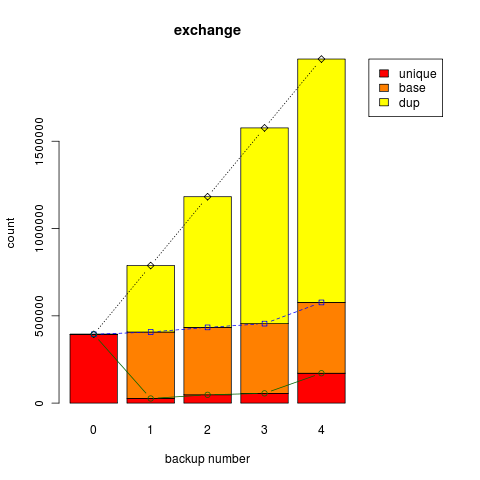
\includegraphics[width=2.5in]{figure/dedup/full011}
\label{ex}}
\hfil
\subfloat[Exchange\_is]{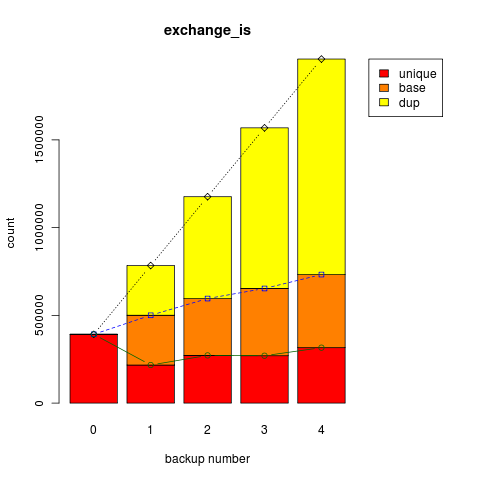
\includegraphics[width=2.5in]{figure/dedup/full012}
\label{ei}}
\hfil
\subfloat[Exchange\_mb]{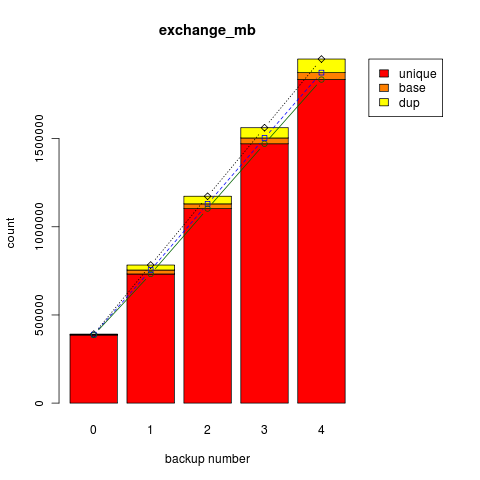
\includegraphics[width=2.5in]{figure/dedup/full013}
\label{em}}}
\centerline{\subfloat[fredp4]{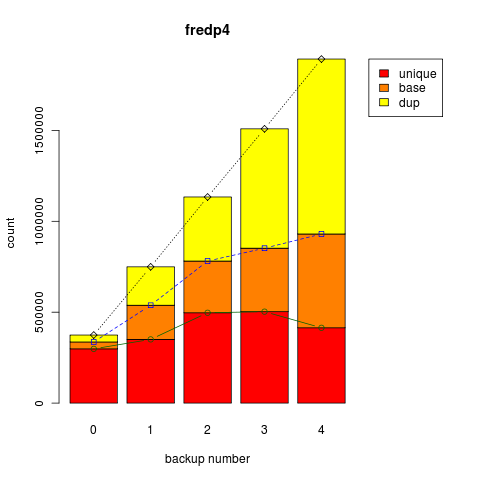
\includegraphics[width=2.5in]{figure/dedup/full014}
\label{fp}}
\hfil
\subfloat[fredvar]{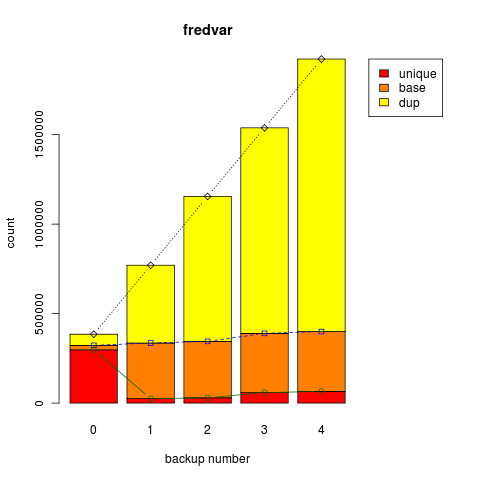
\includegraphics[width=2.5in]{figure/dedup/full015}
\label{fv}}
\hfil
\subfloat[workstation]{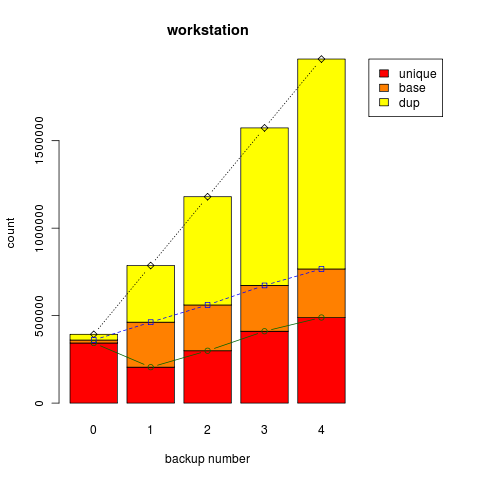
\includegraphics[width=2.5in]{figure/dedup/full016}
\label{ws}}
}
\caption{Composition of segments for different datasets. Graphs show how the composition of segments changes over time as weekly full backups are deduplicated.}
\label{fig_sim}
\end{figure*}

The system parameters for data deduplication system is described in the \tablename~\ref{ex_t}. The cache size for the \emph{content dictionary} is kept reasonably small to capture the effect of cache misses. Since the maximum raw throughput of the system is IO limited at 50MB/s, you can see that the throughput of different datasets vary from being close to the maximum throughput to about 50\% of that throughput. 

As mentioned earlier, there is a strong linear relationship between the compression ratio and the throughput. The sample correlation coefficient, $r_{ct} = -0.98$ (where $c=compression\ ratio$ and $t=throughput$), suggest that higher compression (lower compression ratio) results in higher throughput. While it may seem that compression ratio is the dominant factor in determining the throughput since the two are so highly correlated, the system for which the throughput numbers are reported are \emph{in-line} deduplication systems where all segments must be compared against the content dictionary before it can be stored on the disk. Therefore, the elimination of duplicate segments not only results in dictionary update but also additional disk writes. In systems where data may already all be written to the disk before being looked up in dictionary may not perform in exactly the same manner. Therefore, we concentrate more on dictionary access pattern to analyze potential throughput concerns.

The segment trace contains 5 weekly full backup information of 6 different datasets and 5GB of each full backup. Therefore, all data presented in \tablename~\ref{ds_t} are of the same size at 25GB. The variation in number of segments is due to variation in average segment size. Compression ratio provided in the table is compression due to data deduplication process only and does not include additional compression provided by local compression of segments using traditional data compression tools. 



\section{Data Characterization}\label{result}

An obvious and perhaps the most important data characteristic for data deduplication is amount of redundancy. Two datasets of equal redundancy would yield in similar compression assuming the content generation was done in a reasonable manner. However, they could perform very differently depending on the other aspects such as locality of segments and fragmentation due to elimination of duplicate segments. The difficulty in characterizing workload of data deduplication is that the characteristics is actually dependent on the contents. While access patterns and physical attributes such as size of files tends to follow a well known distributions in a large scale~\cite{riska:2009, leung:2008}, contents themselves are random in nature due to human factor and different encoding deployed by different applications.

\subsection {Composition of Segments}

\begin{figure*}[!t]
\centerline{
\subfloat[Base segments]{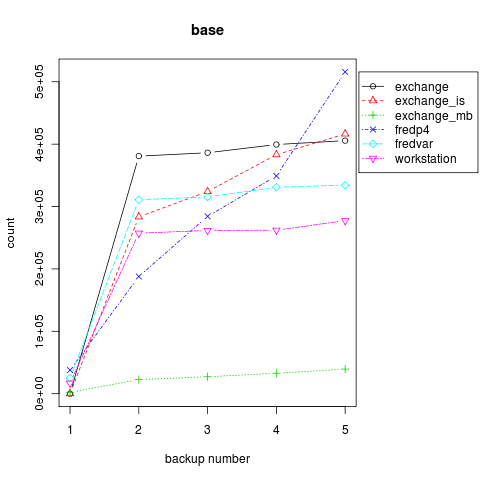
\includegraphics[width=2.5in]{figure/dedup/full005}
\label{bs}}
\hfil
\subfloat[Duplicate segments]{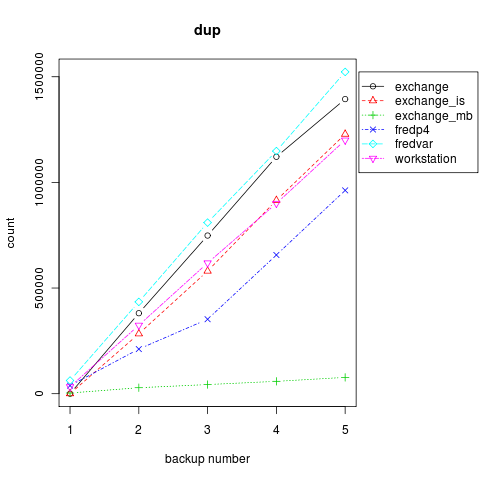
\includegraphics[width=2.5in]{figure/dedup/full002}
\label{ds}}
\hfil
\subfloat[Average references]{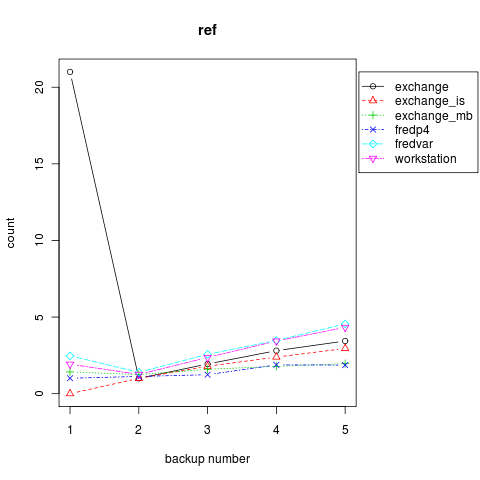
\includegraphics[width=2.5in]{figure/dedup/full009}
\label{ar}}}
\caption{Comparison of data sets. Number of references are simply $|D|/|B|$. Therefore, \emph{exchange\_is} and \emph{frep4} show lowest average number of references since their number of base segments increase with the number of duplicate segments. For all other segments, the number of base segments stay relatively steady indicating that same portion of the data is changing over and over again.}
\label{data_comp}
\end{figure*}

\figurename~\ref{fig_sim} shows how the composition of segments, as defined in \figurename~\ref{seg_class}, changes over time for each dataset at a full backup granularity.  The composition of the segments is quite different for all datasets. In the figure \emph{backup number} represents accumulated number of full backups stored in the system. We make a few observations from the composition.

\begin{observation}\label{1}
Amount of duplication found within a single full backup is negligible compared to the duplication found across the full backups.
\end{observation}

This is an observation also made by other deduplication works on backup data~\cite{kruus:2010}. This observation allows us to look at the changes in the composition of segments as results of deduplicating a full backup instance against other instances of full backup. While non-zero unique and base segments at backup number 0 in \figurename~\ref{fp},  \figurename~\ref{fv} and  \figurename~\ref{ws} indicate that there exists some inter-duplication within a backup, the amount is negligible and we ignore its effect in this paper.

\begin{observation}\label{2}
For the base segments there are two distinctive case where number of base segments increase with number of fulls as in \figurename~\ref{ei} and \figurename~\ref{fp} and case where number of base segments stay steady as shown in \figurename~\ref{ex}, \figurename~\ref{fv} and \figurename~\ref{ws}.
\end{observation}

This observation can be made more pronounced in \figurename~\ref{bs}.

The number of base segments can only increase in the absence of the deletion. Once a segment becomes a base segment, it cannot become any other type of segment. Therefore, the number of base segment can only stay steady if there is no or very little amount of new base segments are created. We can conclude that in this kind of dataset, the unique segments stays unique segments while the same set of base segments keeps getting duplicated.

Conversely, the increase in number of base segments mean that the unique segments of previous backup number is getting converted to the base segments. This happens only when a newly generate data at backup number $i$ still exists at backup number $i+1$. We assume that no base segments are generated within a full backup instance based on the observation \ref{1}. We call this rate of conversion \emph{base generation rate}($bgr$) which is bounded by the number of unique segments in previous backup number and is larger than or equal to 0.

We formally define $bgr$ below.

\begin{definition}[$bgr$]
Rate at which unique segments are converted to base segments. $bgr_i=\frac{|B_{i+1}|-|B_i|}{|U_i|}$ where the subscripts represent the backup number. We define $bgr$ to be average value of $bgr_i$, $bgr = \frac{\sum bgr_i}{max(backup number)}$.
\end{definition}

\begin{observation}\label{3}
The number of unique segments either increase steadily as shown in \figurename~\ref{em} and \figurename~\ref{ws} or stay relatively steady as in the rest of the figures in \figurename~\ref{fig_sim}. While the number of unique segments can decrease, it does not happen very often.
\end{observation}

The number of unique segments, $|U|$, at backup number $i$ is increase by amount of unique segments generated by that particular full backup and is decreased by amount of unique segments at backup number $i-1$ converted to base segments\footnote{Conversion to duplicate segments is also possible but is ignored due to observation \ref{1}.} at backup number $i$. Since the amount of decrease in $|U_{i+1}|$ is $|U_i|\times bgr_i$, we also need to define a parameter to represent the increase in $|U|$, \emph{unique segment ratio}(usr). This ratio does not represent the changes in the number of unique segments, $|U|$, since there is also conversion of segments from unique to base.

\begin{definition}[$\mathit{usr}$]
Relative amount of unique segments within a full backup. $usr_i = \frac{|U_{i+1}|-|U_i|(1-bgr_i)}{|L_{i+1}|}$. We define $\mathit{usr}$ to be average value of $usr_i$, $usr = \frac{\sum usr_i}{max(backup number)}$.
\end{definition}

From the definition of $\mathit{usr}$ it is obvious that we cannot simply determine the rate of unique segment generation from looking at the changes in $|U|$. However, since it is possible to determine the $bgr$ from also looking at the changes in number of base segments, $|B|$ which in turn allow us to calculate $\mathit{usr}$. Since increase in $|B|$ is only possible due to $bgr$, if increase is very small, we can assume that $bgr\simeq0$. This allows us to think that $usr_i=U_{i+1}-U_i$ which means that unique segments in backup number $i$ no longer exists in backup number $i+1$ or else they would have become base segments. This pattern is most pronounced in \figurename~\ref{ws}. Intuitively, the pattern suggests the existence of a small and heavily updated \emph{working set} within the file system as suggested by~\cite{soundararajan:2010}. Similar analysis could applied to \figurename~\ref{em} where almost the entire dataset is a working set. 

Cases where $|B|$ actually increase with the backup number, $bgr$ represents the rate at which new data becomes part of \emph{non-working set}. It suggest that part of the working set becomes stable over time and becomes base on which future segments are deduplicated. Extreme case is shown in \figurename~\ref{fp} where the effect of $bgr$ starts to outweigh the effect of $\mathit{usr}$ and the number of unique segments actually decrease. This is the most desirable case for the data deduplication where amount of data to be store grows sub-linearly and therefore more scalable in terms of backups you can store. It will also be shown that the throughput also tends to be higher in these cases for similar compression.

Cases seen in \figurename~\ref{ex} and \figurename~\ref{fv} suggest that there exists only a small change between the backups. While this is also a desirable case for data deduplication, it may also be argued that for a storage system with such little activity, a longer period of incremental backups could provide similar performance. 

The logical size, $usr$ and $bgr$ of a dataset completely describes the dataset as long as there is no deletion involved. Furthermore, they do not vary as much as $dcr$ over time. Therefore a aggregated values of $usr$ and $bgr$ are much better choices of parameters to describe a dataset. They show how much of new data is generated ($|L|*\overline{\mathit{usr}}$), how much of that data will be changed again before the next full ($1-\mathit{bgr}$). Together, they allow you to calculate the compression ratio at time $i+1$ by following these steps. 
\begin{enumerate}
\item{$|B_{i+1}|=|U_{i}|*\mathit{bgr}_i+|B_i|$.}
\item{$|U_{i+1}|=|L_{i+1}|*\mathit{usr}+|U_i|(1-\mathit{bgr}_i)$.}
\item{Calculate $|D_{i+1}|$ and $\mathit{scr}$ from above two values.}
\end{enumerate}

\subsection{Segment Run Length}

\begin{figure}[!t]
\centering
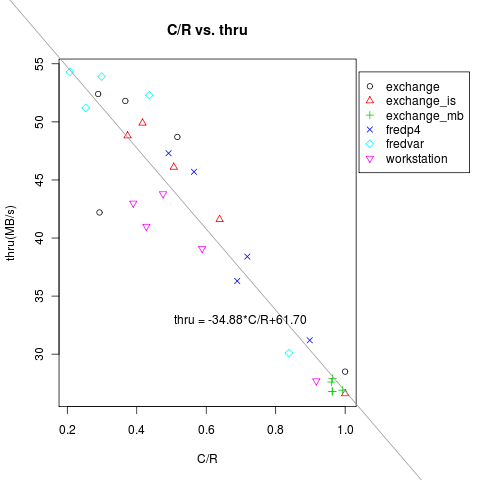
\includegraphics[width=2.5in]{figure/dedup/full018}
\caption{C/R vs. Throughput. The accumulated compression ratio of each dataset at each full backup is plotted against the throughput for that particular backup window. You can observe that the throughput increases as the accumulated compression ratio decreases even though every full backup is equal in size.}
\label{compthru}
\end{figure}

\begin{figure}[!t]
\centering
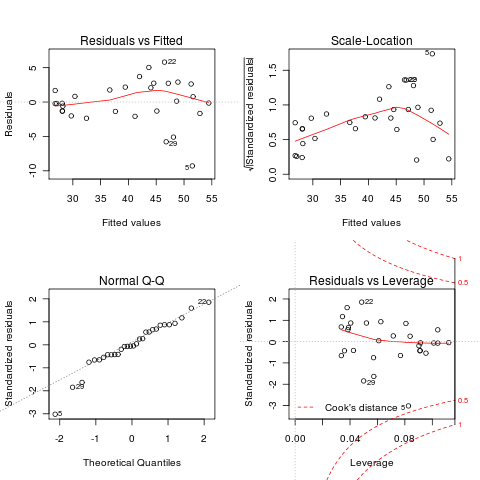
\includegraphics[width=2.5in]{figure/dedup/full019}
\caption{Analysis of C/R vs.throughput. The top left graph shows that while the regression is a good fit, data around throughput value of 40MB/s to 50MB/s tends to out perform expected throughput. Top right graph shows square root of residual error. The backup instance 5, 22 and 29 show a large deviation (from exchange, fredvar and workstation datasets respectively). The lower left graph shows that the residual errors are more or less normally distributed with the exception of 4, 21, 29 (from exchange, exchange\_is and workstation datasets respectively). The lower right graph shows the Cook's distance. Backup instance 5 is less than 0.5 Cook's distance away and can be safely taken into evaluation.} 
\label{anal}
\end{figure}

In section \ref{dss}, we showed that the compression ratio and the throughput of a deduplication system can be highly correlated. \figurename~\ref{compthru} shows throughput vs. compression ratio of each backup instances. This graph together with \figurename~\ref{anal} shows that the compression ratio is indeed a most relevant factor in determining throughput. However, \figurename~\ref{anal} shows some skewness both in Residual vs. Fitted graph and Residual vs. Leverage graph. They suggest at other factors that affect throughput which are not simply white noise. 

\figurename~\ref{compthru} also shows a linear estimation line. One interesting observation is that there are some datasets which perform consistently better than the estimation. These are \emph{exchange\_is}, \emph{fredp4} and \emph{fredvar} datasets. On the other hand, \emph{workstation} dataset performs consistently worse than expected. 

To quantify this effect, we take look at the deviation of throughput numbers from the regression line as shown in \tablename~\ref{dev}. These numbers are not absolute deviation. These are average values of $actual\ throughput - expected\ throughput$ and removes the effect of the compression ratio from the throughput numbers. As explained in section \ref{sys}, the \emph{content dictionary} is the only place where this variation in performance due to content could occur. Note that all data are of the same size, written sequentially once. While \emph{content store} actually stores less if more segments are deduplicated, this performance difference is likely to be linear to the amount of data stored. Since we have removed this linear factor and concentrate only on the deviation, the effect must be due to on content dictionary behavior.

To evaluate the content dictionary behavior, we first look at the sequential runs of segments. A longer sequence of a run represents a sequential access of content dictionary making it easier for the dictionary cache to be a hit. A \emph{run} is simply a sequence of consecutive segments that are either unique or duplicate segments. We refer to them as a \emph{content run} and \emph{duplicate run} respectively when need to distinguish between them. \tablename~\ref{dev} shows aggregated \emph{run} data. We make following observations.

\begin{table}[!t]
\renewcommand{\arraystretch}{1.3}
\caption{Average Deviation from the expected throughput and their corresponding run length information}
\label{dev}
\centering
\begin{tabular}{c||c c c c}
\hline
\bfseries Dataset 	&\bfseries Average	&\bfseries Max		&\bfseries Average	&\bfseries Run Len.	\\
 			&\bfseries Deviation 	&\bfseries Run Len.	&\bfseries Run Len.	&\bfseries $> 1000$	\\		
\hline\hline
fredp4		&1.532			&207400			&7.944			&57\%			\\
exchange\_is	&1.375			&392000			&15.88			&27\%			\\
fredvar		&0.852			&366200			&28.88			&76\%			\\
exchange 		&0.217			&183100			&30.53			&64\%			\\
exchange\_mb 	&-0.722			&7490			&18.6				&13\%			\\
workstation		&-3.260			&5632			&6.635			&9\%				\\			
\hline
\end{tabular}
\end{table}

\begin{observation}
The average run length varies little across the datasets and shows little correlation to the throughput. However, the maximum run length varies significantly across the datasets and show high correlation.
\end{observation}

The correlation coefficient of maximum run length and the average deviation is $r^2 = 0.63$. It is high enough that we can safely assume there is significant correlation between the two values. The correlation coefficient of average run length and the average deviation is only $r^2 = 0.002$. The obvious reason is that the mean values of run length does not represent anything physical when the significant portions of the data lay in outlier regions. The last column of \tablename~\ref{dev} shows that the over 50\% of the segments fall in a run length of over 1000. It is interesting to note that the \emph{fredvar} and \emph{exchange} datasets suffer in throughput even though they have the highest percentage of large runs. It leads us to our next observation.

\begin{observation}
Datasets with high average run length due to many extremely large runs perform worse than cases where the run length are more evenly distributed. 
\end{observation}

The skewed run length has a negative impact on performance not because of the content dictionary but the content store. While it is obvious that less amount to be stored result in high logical throughput as described earlier, the arrival rate of segments to the content store is also important. In a simple queuing model of \figurename~\ref{queue}. Since the arrival rate at the content store is simply $(1-p)S$ where $S$ is the throughput of the content dictionary and $p$ is content dictionary hit probability. If $p$ was uniformly distributed, that the arrival rate would simply be a function of compression ratio. However, as the skewed distribution of run length shows, $p$ of each segments are highly correlated. The effect is bursty arrivals at the content sore resulting in high queue length and lower throughput as shown in \figurename~\ref{ql}. It is shown that the effect of run length is less pronounced for datasets with higher compression ratio. The \emph{all\_miss} case is the worst case where every segment is sent to the segment store and \emph{rand} is the best case where run length distribution is uniform.
 
\begin{figure}[!t]
\centering
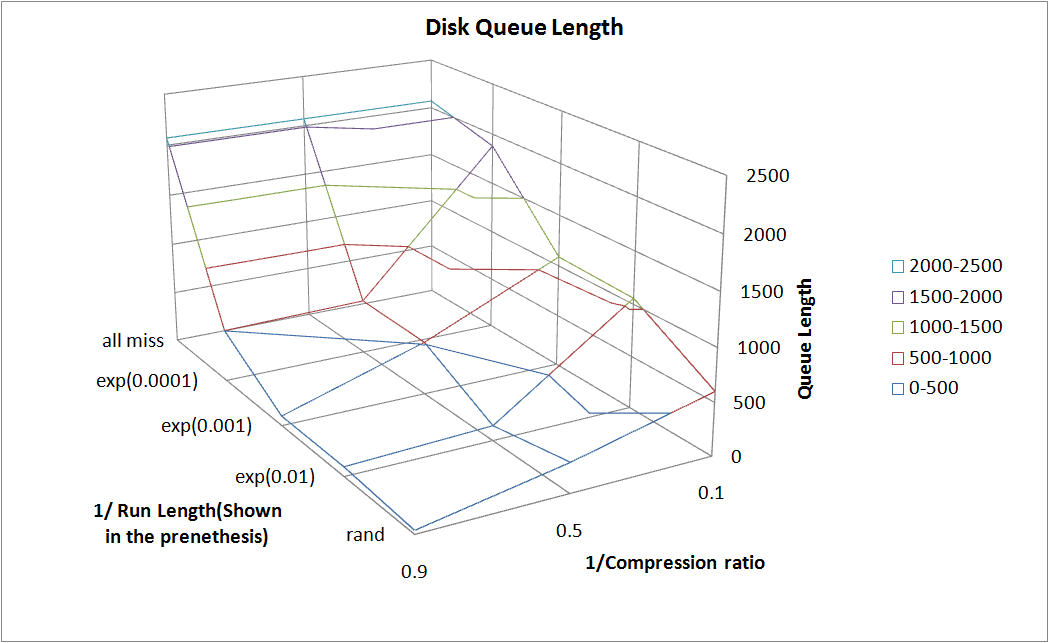
\includegraphics[width=3in]{figure/dedup/disk_q}
\caption{Run length vs. compression ratio vs. queue length.}
\label{ql}
\end{figure}

The run length analysis shows that while the throughput is highly correlated with the compression ratio, higher run length typically results in higher throughput. Additionally, skewed run length which typically results from few very long runs, results in lower throughput especially when the compression ratio is low.

\section{Applications}\label{appp}
Above analysis of composition of segments allows users of deduplication systems to collect specific statistics to predict future storage requirements. In the world of deduplication where the physical storage space and the logical segment space does not match, it is difficult to provision storage space. Extracting $bgr$ and $usr$ from the deduplicated data allow users to better predict future storage requirements. 

For the given six test datasets, we use $bgr$ and $usr$ of the first three fulls to predict the comression ratio of 4th and 5th full and compare them with the $dcr$ approach.

For example, the $bgr_1\sim 0.01$ and $usr_1\sim 0.26$ for \emph{workstation} dataset. Since $|L_i|\sim393311$,  we can predict future segment composition given backup number 2 information. \figurename~\ref{pred} shows the graph of the original workstation composition and the graph of predicted composition. Since the parameters were extracted from the backup number 1 and 2, the accuracy of prediction falls as the number of fulls increase. Of course, the accuracy of the prediction itself is also dependent on the dataset and the worst case error was observed in \emph{exchange} dataset where the $\mathit{scr}$ at backup 4 was off by just over 0.02($\sim5\%$ error). This is much better approach than simply observing the compression ratio. For \emph{fredp4} dataset the $dcr$  prediction is off in compression ratio by 0.18 ($\sim36\%$ error).

\begin{table}[!t]
\renewcommand{\arraystretch}{1.3}
\caption{Compression ratio prediction error comparison}
\label{err}
\centering
\begin{tabular}{c||c c}
\hline
\bfseries datasets &\bfseries dcr	 	&\bfseries usr \& bgr	\\
\hline\hline
fredp4		&35.99\%			&3.68\%					\\
exchange\_is	&9.20\%			&2.21\%				\\
fredvar		&7.35\%			&0.21\%						\\
exchange 		&17.82\%			&5.42\%					\\
exchange\_mb 	&0.14\%			&0.20\%				\\
workstation		&3.61\%			&0.61\%				\\			
\hline
\end{tabular}
\end{table}

\tablename~\ref{err} shows our approach outperforms the tradistional $dcr$ approach in all but exchange\_mb dataset where the error is about the same.

Another potential application is evaluating the impact of merging two separately deduplicated data. Unless there is a reason to suspect a large similarity between the two datasets, parameters of each dataset can be superpositioned to predict the composition of combined dataset. 

A more involved application would be to filter out the \emph{working set} from being deduplicated. Various techniques exists to evaluate the working set of a storage system~\cite{lee:2009, wang:2004} which can be used to identify \emph{hot data} and pass only those deemed cold to the deduplication system. This would be especially useful for datasets with low $bgr$ where same portions of the data are constantly changing. This portion can deemed unworthy of deduplication and is backed up separately. 

The analysis of run length suggest that it maybe more beneficial for the through put if the inter-duplicate segments are ignored. That is we only evaluate duplicate segments generated between the full backups. These single or dual duplicate segments fragment the index table and potentially the contents on disk without providing any substantial gain in compression. 

Last application maybe to adjust buffer sizes at each stage of deduplication based on the run length observed to minimized skewed arrival effect. 

 \begin{figure}[!t]
\centerline{
\subfloat[Real Data]{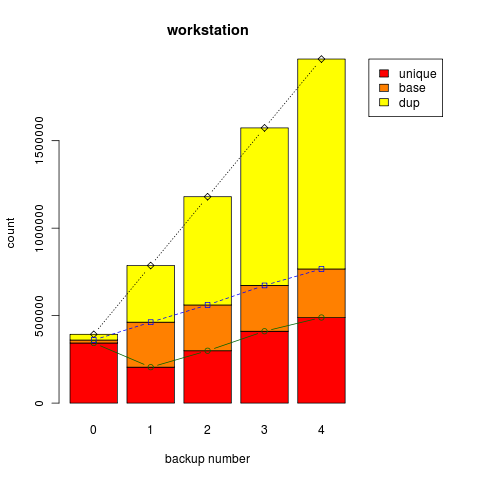
\includegraphics[width=1.9in]{figure/dedup/full016}
\label{wo}}
\hfil
\subfloat[Predicted Data]{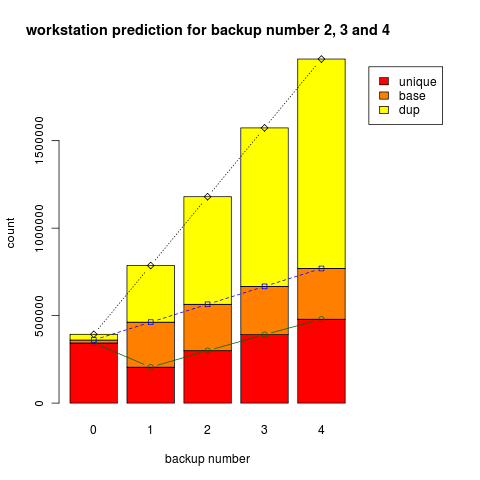
\includegraphics[width=1.9in]{figure/dedup/prediction001}
\label{wp}}
}
\caption{The original segment composition of workstation and the predicted values.}
\label{pred}
\end{figure}

\section{Limitations}\label{lim}
%%Assumptions - second assumption can be proven with in statistical margin.
Many deduplication systems allow the segments to be stored without duplicate detection for the better throughput~\cite{bhagwat:2009, lillibridge:2009}. This does not cause correctness issue. However, it makes predicting performance even more difficult. In this study we assume that all duplicate segments must be identified and eliminated. There has also been attempts to make better decisions on identifying the data segments from the dataset~\cite{eshghi:2005, kruus:2010, bobbarjung:2006}. We claim that the segments, regardless of how they are defined, define datasets in terms of data deduplication process. This claim assumes that different datasets will have statistically similar relative compression and performance regardless of the segmentation process. In other words, segmentation process affects different dataset in statistically similar way. For example, if dataset $A$ gained compression ratio by 10\% while losing throughput by 5\% by using the new segmentation method, than dataset $B$ is highly probable to gain in compression and lose in throughput by similar amount. While this assumption is actually verifiable, lack of datasets prevents us from providing strong statistical guarantee. However, previous analysis of segmentation algorithms~\cite{kruus:2010} as well as our own tests indicate no evidence to reject our assumption.

\section{Conclusion}\label{con}
We have shown a framework for characterizing datasets by analyzing how different datasets behave within a data deduplication system. For the datasets presented here, we show that there are classes of datasets which behave similarly.

We also show that the changes in the number of base segments is more important in terms of scalable data compression than the simple compression ratio. More specifically, a positive $bgr$ guarantees continuing reduction in the compression ratio resulting in sub-linear growth in the storage requirement. Intuitively, $bgr$ represents life time of new data. High $bgr$ means that newly created data are long lived and low $bgr$ means that they are short lived. Since $usr$ represents amount of new data created, their ratio tells you how much of the new data is transient and how much are more permanent. Generating more and more permanent data means more data to be deduplicated at each back up resulting in better compression ratio.  

We also show that the segment run length has a fundamental effect on the dictionary lookup process both in terms of the cache behavior and queuing delays, which can counteract each other in terms of throughput. More specifically, the typical belief that high average run length results in better throughput is not true. In fact, it can lower the throughput due to skewed arrival rate the content store. However, high maximum run length tends to improve performance due to good caching effect of content dictionary. Simply put, one can estimate throughput based on the compression ratio using a C/R vs. throughput regression line for a given system and can further expect the throughput to be better or worse based on the run length information.

Lastly, we showed that we can increase the accuracy of compression ratio prediction by as much as 80\%. Furthermore, we can accurately predict the composition of segments which allow us to determine the existence of frequently updated data which does not have to be deduplicated. 

%%%%%%%%%%%%%%%%%%%%%%%%%%%%%%%%%%%%%%%%%%%%%%%%%%%%%%%%%%%%%%%%%%%%%%%%%%%%%%%%
       % backup workloads
%%%%%%%%%%%%%%%%%%%%%%%%%%%%%%%%%%%%%%%%%%%%%%%%%%%%%%%%%%%%%%%%%%%%%%%%%%%%%%%%
%related.tex: Related works
%%%%%%%%%%%%%%%%%%%%%%%%%%%%%%%%%%%%%%%%%%%%%%%%%%%%%%%%%%%%%%%%%%%%%%%%%%%%%%%%
\chapter{Related Work}
\label{RELATED}
%%%%%%%%%%%%%%%%%%%%%%%%%%%%%%%%%%%%%%%%%%%%%%%%%%%%%%%%%%%%%%%%%%%%%%%%%%%%%%%%
\section{Storage IO Workload Characterization}

Characterizing the workload for storage subsystems started as early as 1965 in order to simulate computer system performance~\cite{hutchinson:1965}. 
For almost two decades, the main focus of the characterization was on the arrival rate of IO requests~\cite{hutchinson:1965, fuchel:1967, reddy:1989}. 
Hence, a simple queueing model was used to describe storage system behavior~\cite{kleinrock:1975}. 

At around the same time, synthetic benchmarks that takes record sizes, number of records, read rate, write rate and number of files became available~\cite{park:1990, wolman:1989}.
A plateau of works on measuring real workloads in production systems followed~\cite{ruemmler:1993, kavalanekar:2008, ahmad:2007, wang:2009, roselli:2000, calzarossa:1993, smirni:1997, calzarossa:2000, arlitt:1996, riska:2006}. 
Consequently, comprehensive and complex storage models~\cite{anderson:1968,brichet:1996,copeland:1985,freeman:1996,norros:1994} as well as storage benchmarks followed~\cite{traeger:2008}. 

Importance of locality in sub storage systems was shown to be important in the 80's~\cite{ousterhout:1985}. 
However, the efforts to quantify locality in storage systems have began only recently. 
Two different approaches exists. 
One approach relies on the fact that the autocorrelation of LBN sequence tends not to decay exponentially~\cite{denning:1972}.
This effect is known as the \emph{long memory} effect and can be quantified using \emph{Hurst exponent}~\cite{gomez:2000}.
The other approach takes a more traditional approach of \emph{Stack Distance}~\cite{mattson:1970} and \emph{Seek Distance}~\cite{fox:2008}.

These new ways of describing workloads allows us to gain new insights into the workloads.
However, previous works have failed to link these new characteristics to the way the workloads interact with storage systems rendering the insights to be somewhat interesting but less useful.

There exists another set of characterization that relies on extracting a set of components from the workload so that the workload can be sythetically generated~\cite{sreenivasan:1974}.
Theses techniques typically rely on unintutive parameters that cannot be meaning fully controlled.
Therefore the application of these characrteristics are limited to replaying a specific trace only.



\section{Locality}
\label{LOCAL}

%traditional locality

%temporal locality

%spatial locality

%long memory process




\section{Data Deduplication}
\label{DD}

The workload presented in typical deduplication systems paper are either from a privately accessible systems~\cite{clements:2009, rhea:2008, manber:1994, aronovich:2009, lillibridge:2009, zhu:2008} or a relatively small dataset of specific type in public domain~\cite{storer:2008, kruus:2010, eshghi:2005}. 
However, either techniques allow a direct comparison of different systems if the dataset under evaluation is completely different or if it only covers a dataset of a particular characteristics.

There have been few work in trying to statistically characterize the input dataset to various benchmark programs~\cite{eeckhout:2003, yi:2002, hsu:2002}. 
However, these papers concentrate on generic sub-setting of dataset so that different characteristics of application is explored statistically hence lacking in accuracy when it comes to predicting exact performance variances.

Numerous works have also been applied in filesystem activities and its contents~\cite{douceur:1999, leung:2008, douceur:1999} with one paper using a simple statistical analysis to characterize a filesystem impression~\cite{agrawal:2009}. 
While these approaches all reveal some interesting intuitions of how we use storage systems, the scope is too generic to be neither accurate or simple enough to be applied in real systems. 
More specific workload analysis have been targeted to SSDs~\cite{soundararajan:2010} and we use some of their approach in out analysis.

\section{IO Benchmark Programs}

%iozone

%iometer

%fio

%vdbench

%bonnie++



\section{Storage Virtualization}
\label{SV}

%lvm

%virtual disks

%thin provisioning

%consolidation

%%%%%%%%%%%%%%%%%%%%%%%%%%%%%%%%%%%%%%%%%%%%%%%%%%%%%%%%%%%%%%%%%%%%%%%%%%%%%%%%
 
%%%%%%%%%%%%%%%%%%%%%%%%%%%%%%%%%%%%%%%%%%%%%%%%%%%%%%%%%%%%%%%%%%%%%%%%%%%%%%%%
% conclusion.tex:
%%%%%%%%%%%%%%%%%%%%%%%%%%%%%%%%%%%%%%%%%%%%%%%%%%%%%%%%%%%%%%%%%%%%%%%%%%%%%%%%
\chapter{Conclusion and Discussion}
\label{conclusion_chapter}
%%%%%%%%%%%%%%%%%%%%%%%%%%%%%%%%%%%%%%%%%%%%%%%%%%%%%%%%%%%%%%%%%%%%%%%%%%%%%%%%
We have presented Romano, a load balancing framework for virtual disks
on heterogeneous storage systems. The kernel of Romano is a performance
predictor given a set of parameters that characterize the workloads and
the storage devices. We have shown that Romano can outperform
previous systems with same goals by up to 80\% in prediction
accuracy. This increased accuracy results in 78\% reduction in maximum
latency observed and 82\% reduction in variance while load balancing.

At a deeper level, Romano contributes a recognition that there is
inherent noise in storage system performance that is not easily dealt
with. Romano is capable of capturing this noise within the prediction
interval. As more data is gathered there is higher confidence that the
prediction interval will contain the measured latency. 

Another key contribution of Romano is quantification of effect of
various workload characteristics and their interaction on heterogeneous
storage devices. 
We have shown that the performance differences between data stores cannot be described with a single number. More specifically, we have shown that the storage performance must be described in terms of the workload.

The last contribution follows the second contribution. Since the performance of storage systems effectively change with the workload, the load balancing problem is no longer a bin-packing problem as previously believed. 
Therefore we present a probabilistic approach to finding a pseudo-optimal mapping of workloads to the data stores. 
It is important to mention that probabilistic approach is only used to find the final state of the system and the moves are actually made greedily to speed up the convergence and minimize the number of moves that has to be made.

We believe that Romano not only provides means for more efficient load
balancing but also in many other areas such as QoS management, power management and performance tunning in tiered storage.

Whereas Romano raises the bar on the accuracy of practical modeling
techniques, there remain ample opportunities for improvements in
future work. Better interference modeling between workloads when they
are placed on same data store is one such area where we are making
good progress. Another work in progress is to come up with a better
set of workload characteristics such that the workload description can
be more complete.
%%%%%%%%%%%%%%%%%%%%%%%%%%%%%%%%%%%%%%%%%%%%%%%%%%%%%%%%%%%%%%%%%%%%%%%%%%%%%%%%

%%%%%%%%%%%%%%%%%%%%%%%%%%%%%%%%%%%%%%%%%%%%%%%%%%%%%%%%%%%%%%%%%%%%%%%%%%%%%%%%

%%%%%%%%%%%%%%%%%%%%%%%%%%%%%%%%%%%%%%%%%%%%%%%%%%%%%%%%%%%%%%%%%%%%%%%%%%%%%%%%
% Bibliography, uncomment for final version
%%%%%%%%%%%%%%%%%%%%%%%%%%%%%%%%%%%%%%%%%%%%%%%%%%%%%%%%%%%%%%%%%%%%%%%%%%%%%%%%
\bibliography{thesis}
%%%%%%%%%%%%%%%%%%%%%%%%%%%%%%%%%%%%%%%%%%%%%%%%%%%%%%%%%%%%%%%%%%%%%%%%%%%%%%%%

%%%%%%%%%%%%%%%%%%%%%%%%%%%%%%%%%%%%%%%%%%%%%%%%%%%%%%%%%%%%%%%%%%%%%%%%%%%%%%%%
% End the Document
%%%%%%%%%%%%%%%%%%%%%%%%%%%%%%%%%%%%%%%%%%%%%%%%%%%%%%%%%%%%%%%%%%%%%%%%%%%%%%%%
\end{document}
%%%%%%%%%%%%%%%%%%%%%%%%%%%%%%%%%%%%%%%%%%%%%%%%%%%%%%%%%%%%%%%%%%%%%%%%%%%%%%%%
